\documentclass[fleqn,11pt]{report}
% ********************************************************************
% ********************************************************************
% package for Cosserat materials in chapter ch-nonlinear-material-modeling
\usepackage{bm}
\usepackage{ mathrsfs }
\usepackage{ upgreek }
% ********************************************************************
% ********************************************************************
% pakage for chapter ch-vesion-stability
\usepackage{graphicx}
\usepackage{lastpage}
\usepackage{fancyhdr}
\usepackage{float}
\usepackage{caption}
\usepackage{subcaption}
\usepackage{color}
\usepackage[utf8]{inputenc}
\usepackage[T1]{fontenc}
\usepackage{textcomp}
\usepackage{gensymb}
\usepackage{amsmath}
\usepackage{multirow}
\usepackage{hyperref}

% ********************************************************************
% ********************************************************************
% list and color setting
\usepackage{color}
\usepackage{xcolor}
\usepackage{listings}
\lstloadlanguages{Matlab,Python,bash,make,C++}
% \input{latex_fei_highlight}

% ********************************************************************
% ********************************************************************
% pakage for chapter ch-Constitutive_Application_of_Small_linear_algebra_in_Elastoplastic_Algorithms
\usepackage{tcolorbox}
\usepackage{algorithm}
\usepackage{algpseudocode}
\lstset{language=C++,
                basicstyle=\ttfamily,
                keywordstyle=\color{blue}\ttfamily,
                stringstyle=\color{red}\ttfamily,
                commentstyle=\color{gray}\ttfamily,
                morecomment=[l][\color{magenta}]{\#}
}

% ********************************************************************
% ********************************************************************
% pakage for chapter ch-manufactured_solution_paper
\usepackage{enumitem}
\setlist[description]{leftmargin=\parindent,labelindent=\parindent}
\usepackage[numbers]{natbib}
\usepackage{bm}

% ********************************************************************
% ********************************************************************
% pakage for chapter ch-compare-diff-compilers
\usepackage{tabularx}



% ********************************************************************
% ********************************************************************
% Page boundary setting
\setlength{\textwidth}{17.5cm}
\setlength{\textheight}{23.2cm}
\setlength{\hoffset}{-2.0cm}
\setlength{\voffset}{-2.5cm}

% ********************************************************************
% ********************************************************************
% Date and Time setting
\def\today
{\number\day.\space \ifcase\month\or
January\or
February\or
March\or
April\or
May\or
June\or
July\or
August\or
September\or
October\or
November\or
December\fi,\space
\number\year}

\newcount\hh
\newcount\mm
\mm=\time
\hh=\time
\divide\hh by 60
\divide\mm by 60
\multiply\mm by 60
\mm=-\mm
\advance\mm by \time
\def\hhmm{\number\hh:\ifnum\mm<10{}0\fi\number\mm}

% ********************************************************************
% ********************************************************************
% Page head and Page foot setting
\lhead{\small \it Real-ESSI Short Courses Examples}
\chead{\small \it }
\rhead{\small \it \thepage{} of \pageref{LastPage} }
\lfoot{\small \it University of California}
\rfoot{\small \it \today, \hhmm}
\cfoot{\small \it  }
\addtolength{\headheight}{14pt}

% ********************************************************************
% ********************************************************************
% Table setting.
\newcommand{\tabincell}[2]{\begin{tabular}{@{}#1@{}}#2\end{tabular}}

\pagestyle{fancy}

% ********************************************************************
% ********************************************************************
% Begin document
\begin{document}

% ********************************************************************
% ********************************************************************
\begin{titlepage}
	\centering
	% \includegraphics[width=0.15\textwidth]{example-image-1x1}\par\vspace{1cm}
	{\scshape\LARGE University of California and  \par}
	\vspace{1cm}
	{\scshape\Large Lawrence Berkeley National Laboratory \par}
	\vspace{1.5cm}
	{\huge\bfseries 
		Real-ESSI Short Course Examples  
	\par}
	\vspace{2cm}
	% {\Large Yuan \textsc{Feng}\par}
	% ofeng@ucdavis.edu
	\vfill
	% supervised by\par
	% Prof.~Boris \textsc{Jeremi\'{c}}

	\vfill
	
	{
		\begin{center}
		\item Day 1: Overview
		\item Day 2: Motions
		\item Day 3: Nonlinearity
		\end{center}
	}
	\vfill

% Bottom of the page
	{\large \today\par}
\end{titlepage}
% ********************************************************************
% ********************************************************************
% The second page:
\tableofcontents{}

% % The Abstract page:
% \clearpage\newpage
% \begin{center}
% \item{\large \itshape \textbf {Abstract}}
% \end{center}

% ********************************************************************
% The chapters:
% ********************************************************************
\chapter{Introduction}
\label{ch_Introduction}

Real-ESSI is constructed with x2go remote desktop on Amazon Web Service (AWS).
To use the Real-ESSI cloud service, users need to install the x2go client 
on their operating systems.

\section{Install x2go client}
Before connect to Real-ESSI cloud, users should install the client-side of x2go.

\subsection{Install the client-side of x2go}
\paragraph{Install x2go client on Ubuntu} ~

\begin{lstlisting}[frame=single,language=bash]
sudo apt install -y x2goclient
\end{lstlisting}
\paragraph{Install x2go client on Mac}
Users can download the package through this link: 
\url{http://code.x2go.org/releases/X2GoClient_latest_macosx_10_9.dmg}.

\paragraph{Install x2go client on Windows}
Users can download the package through this link: 
\url{http://code.x2go.org/releases/X2GoClient_latest_mswin32-setup.exe}.

\paragraph{Install x2go client on other operating systems}
If you are using a different operating system, please refer to x2go 
website for the installation. The x2go website for client installation 
is \url{https://wiki.x2go.org/doku.php/download:start}

\subsection{Configure the client-side of x2go}

For all operating systems, users will see the same session when they
open the x2goclient new-session, as shown in Fig.~\ref{fig_x2go_client}.

\begin{figure}[H]
  \centering
  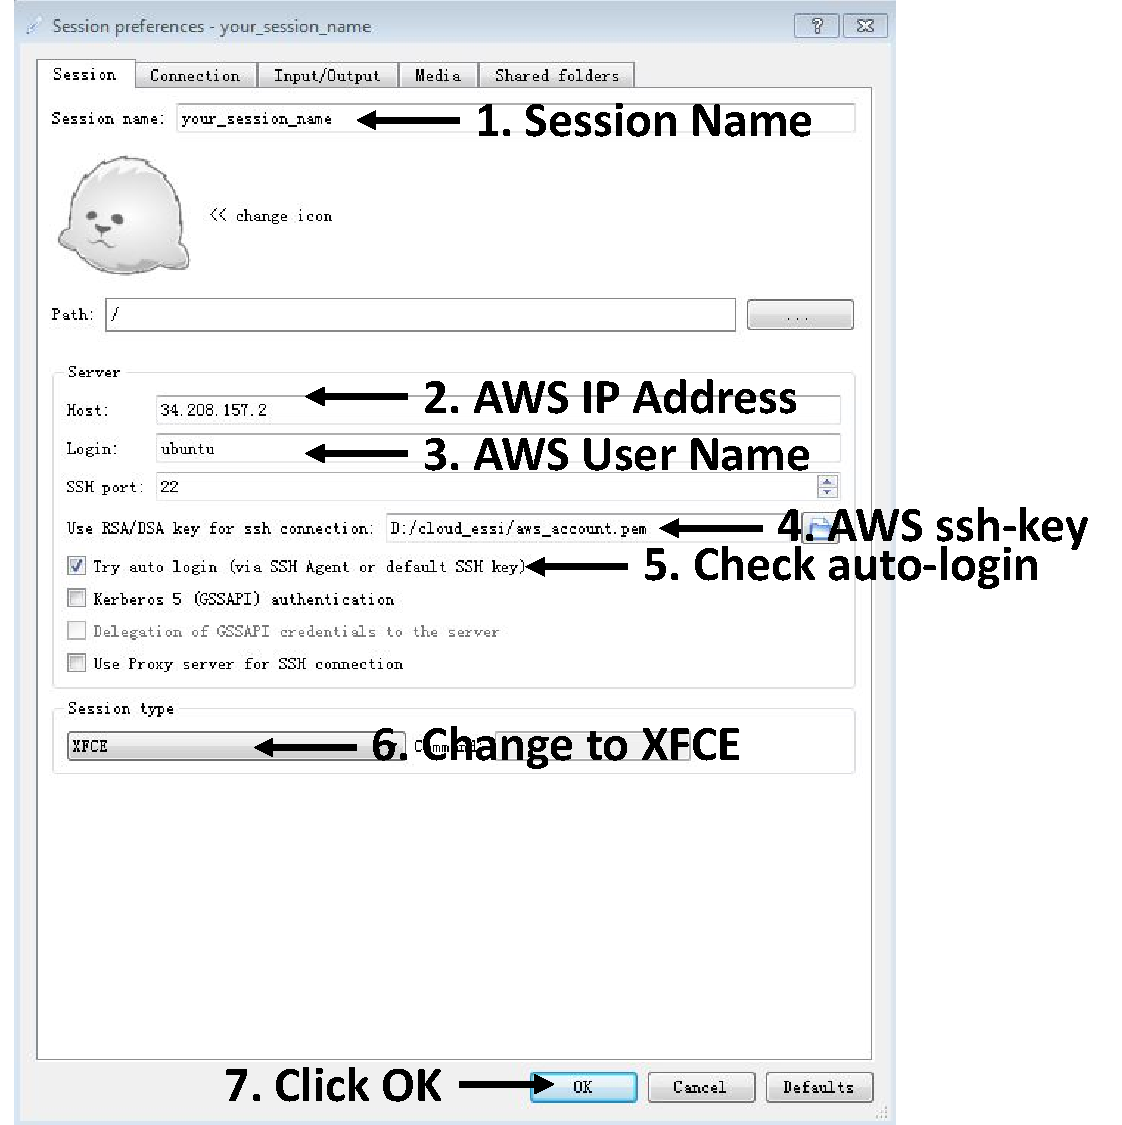
\includegraphics[width = 9cm]{./Figure-files/overview/login_windows_x2go.pdf}
  \caption{Configuration of x2go client}
  \label{fig_x2go_client}
\end{figure}

\begin{enumerate}
	\item Users can name their own session name.
	\item AWS IP address will be provided in the Real-ESSI Short-Course.
	\item AWS User Name is "ubuntu".
	\item AWS ssh-key will be provided in the Real-ESSI Short-Course.
	\item Please check the auto-login.
	\item Please change the session type to XFCE.
	\item Click OK to finish the configuration.
\end{enumerate}

% \section{AWS Regions}

% \subsection{AWS Price by Regions}
% Choosing an AWS region is the first decision you have to make when you set up 
% your AWS components. Most AWS customers choose one based on proximity to 
% themselves or to their end users, which sounds like a sensible thing to do.
% However, proximity alone is not enough.
% The price is also important. 
% An example of AWS price by regions is shown in Fig.~\ref{fig_aws_price_by_regions}. 
% The example is for 10 t2.medium instances running Amazon Linux in the same 
% Availability Zone. Each instance has 20GB of EBS SSD storage. 

% \begin{figure}[H]
%   \centering
%   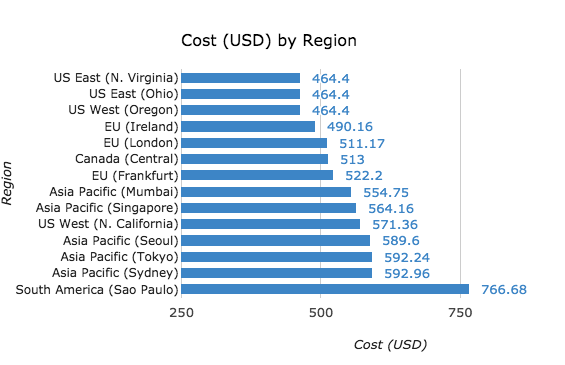
\includegraphics[width = 10cm]{./Figure-files/overview/aws-price-chart.png}
%   \caption{AWS Price by Regions}
%   \label{fig_aws_price_by_regions}
% \end{figure}


% \subsection{AWS Latency by Regions}
% Regions have different latencies and data transfer speeds. 
% An example of AWS latencies by regions is shown in Fig.~\ref{fig_aws_latency_by_regions}.
% The example is a test that measures latency between EC2 instances in different regions.
% For example, from North California it took 2ms to ping EC2 instances in North California,
% and it took 41ms to ping EC2 instances in Oregon.

% \begin{figure}[H]
%   \centering
%   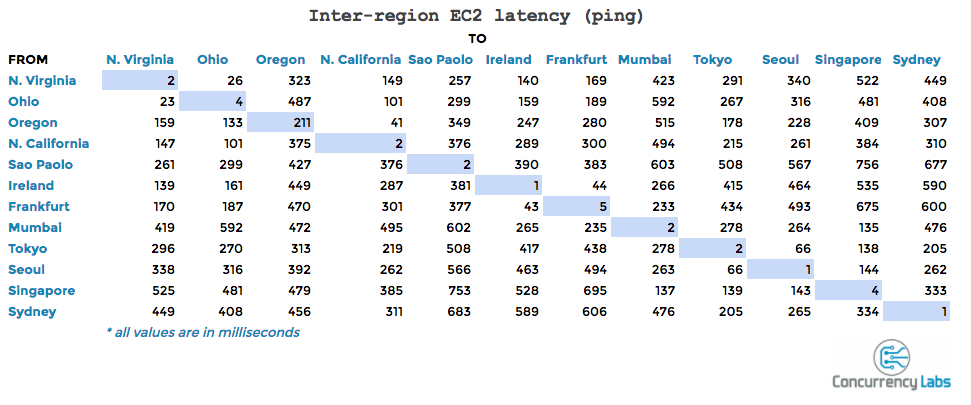
\includegraphics[width = 14cm]{./Figure-files/overview/ec2-ping-table.png}
%   \caption{AWS Latency by Regions}
%   \label{fig_aws_latency_by_regions}
% \end{figure}






\chapter{Day 1 Overview}
\label{ch-day1}

% ******************************************************************
% ******************************************************************
% ******************************************************************
\clearpage
\newpage
\section{Nuclear Power Plant with 3D motions from SW4}
\label{Nuclear_Power_Plant_with_3D_motions_from_SW4}

The Real-ESSI input files for this example are available 
\href{http://sokocalo.engr.ucdavis.edu/~jeremic/lecture_notes_online_material/_Chapter_Short_Course_Examples/short-course-examples/Day1/Nuclear_Power_Plant_with_3D_motions_from_SW4}{HERE}. 
The compressed package of Real-ESSI input files for this example is available 
\href{http://sokocalo.engr.ucdavis.edu/~jeremic/lecture_notes_online_material/_Chapter_Short_Course_Examples/short-course-examples/Day1/Nuclear_Power_Plant_with_3D_motions_from_SW4/_all_files_packaged_for_Nuclear_Power_Plant_with_3D_motions_from_SW4.tar.gz}{HERE}. 

\begin{figure}[H]
  \centering
  \includegraphics[width = 9cm]{./Figure-files/Day1/Nuclear_Power_Plant_with_3D_motions_from_SW4/overview.png}
  \caption{Simulation Model}
  \label{fig_NPP_3D_overview_3D_motion}
\end{figure}

The Modeling parameters are listed.
\begin{itemize}
  \item Soil 
  \begin{itemize}
    \item Unit weight, $\gamma$, \enspace \enspace 21.4 kPa
    \item Shear velocity, $Vs$, \enspace \enspace 500 m/s
    \item Young's modulus, $E$, \enspace \enspace 1.3 GPa
    \item Poisson's ratio, $\nu$, \enspace \enspace 0.25
    \item Shear strength, $S_u$, \enspace \enspace 650 kPa
    \item von Mises radius, $k$, \enspace \enspace 60 kPa
    \item kinematic hardening, $H_a$, \enspace \enspace 30 MPa
    \item kinematic hardening, $C_r$, \enspace \enspace 25
  \end{itemize}
  \item Structure
  \begin{itemize}
    \item Unit weight, $\gamma$, \enspace \enspace 24 kPa
    \item Young's modulus, $E$, \enspace \enspace 20 GPa
    \item Poisson's ratio, $\nu$, \enspace \enspace 0.21
  \end{itemize}
\end{itemize}

The input motion at the bottom is a 3D wave from SW4.

SIMULATION TIME: With 32 cores on AWS EC2 c4.8xlarge instance, the running time for this example is 17 hours.

% ******************************************************************
% ******************************************************************
% ******************************************************************
\clearpage
\newpage
\section{Nuclear Power Plant with 1D motions from Deconvolution}
\label{Nuclear_Power_Plant_with_1D_motions_from_Deconvolution}

The Real-ESSI input files for this example are available 
\href{http://sokocalo.engr.ucdavis.edu/~jeremic/lecture_notes_online_material/_Chapter_Short_Course_Examples/short-course-examples/Day1/Nuclear_Power_Plant_with_1D_motions_from_Deconvolution}{HERE}. 
The compressed package of Real-ESSI input files for this example is available 
\href{http://sokocalo.engr.ucdavis.edu/~jeremic/lecture_notes_online_material/_Chapter_Short_Course_Examples/short-course-examples/Day1/Nuclear_Power_Plant_with_1D_motions_from_Deconvolution/_all_files_packaged_for_Nuclear_Power_Plant_with_1D_motions_from_Deconvolution.tar.gz}{HERE}. 

\begin{figure}[H]
  \centering
  \includegraphics[width = 7cm]{./Figure-files/Day1/Nuclear_Power_Plant_with_1D_motions_from_Deconvolution/overview.png}
  \caption{Simulation Model}
  \label{fig_NPP_3D_overview_1D_motion}
\end{figure}

The input motion at the bottom is the deconvolution of the Northridge earthquake records. 

\begin{figure}[H]
  \centering
  \includegraphics[width = 7cm]{./Figure-files/Day1/Nuclear_Power_Plant_with_1D_motions_from_Deconvolution/scaled_NORTHR_x_A.jpg}
  \includegraphics[width = 7cm]{./Figure-files/Day1/Nuclear_Power_Plant_with_1D_motions_from_Deconvolution/scaled_NORTHR_x_D.jpg}
  \caption{Motion Deconvolution}
  \label{fig_motion_deconvolution1}
\end{figure}

The Modeling parameters are listed.
\begin{itemize}
  \item Soil 
  \begin{itemize}
    \item Unit weight, $\gamma$, \enspace \enspace 21.4 kPa
    \item Shear velocity, $Vs$, \enspace \enspace 500 m/s
    \item Young's modulus, $E$, \enspace \enspace 1.3 GPa
    \item Poisson's ratio, $\nu$, \enspace \enspace 0.25
    \item Shear strength, $S_u$, \enspace \enspace 650 kPa
    \item von Mises radius, $k$, \enspace \enspace 60 kPa
    \item kinematic hardening, $H_a$, \enspace \enspace 30 MPa
    \item kinematic hardening, $C_r$, \enspace \enspace 25
  \end{itemize}
  \item Structure
  \begin{itemize}
    \item Unit weight, $\gamma$, \enspace \enspace 24 kPa
    \item Young's modulus, $E$, \enspace \enspace 20 GPa
    \item Poisson's ratio, $\nu$, \enspace \enspace 0.21
  \end{itemize}
\end{itemize}

% ******************************************************************
% ******************************************************************
% ******************************************************************
\clearpage
\newpage
\section{Nuclear Power Plant with 3$\times$1D motions from Deconvolution}
\label{Nuclear_Power_Plant_with_3by1D_motions_from_Deconvolution}

The Real-ESSI input files for this example are available 
\href{http://sokocalo.engr.ucdavis.edu/~jeremic/lecture_notes_online_material/_Chapter_Short_Course_Examples/short-course-examples/Day1/Nuclear_Power_Plant_with_3by1D_motions_from_Deconvolution}{HERE}. 
The compressed package of Real-ESSI input files for this example is available 
\href{http://sokocalo.engr.ucdavis.edu/~jeremic/lecture_notes_online_material/_Chapter_Short_Course_Examples/short-course-examples/Day1/Nuclear_Power_Plant_with_3by1D_motions_from_Deconvolution/_all_files_packaged_for_Nuclear_Power_Plant_with_3by1D_motions_from_Deconvolution.tar.gz}{HERE}. 

\begin{figure}[H]
  \centering
  \includegraphics[width = 9cm]{./Figure-files/Day1/Nuclear_Power_Plant_with_3by1D_motions_from_Deconvolution/overview.png}
  \caption{Simulation Model}
  \label{fig_NPP_3D_overview_3by1Dmotion}
\end{figure}


The input motion at the bottom is the deconvolution of the Northridge earthquake records. 

\begin{figure}[H]
  \centering
  \includegraphics[width = 5cm]{./Figure-files/Day1/Nuclear_Power_Plant_with_3by1D_motions_from_Deconvolution/scaled_NORTHR_x_A.jpg}
  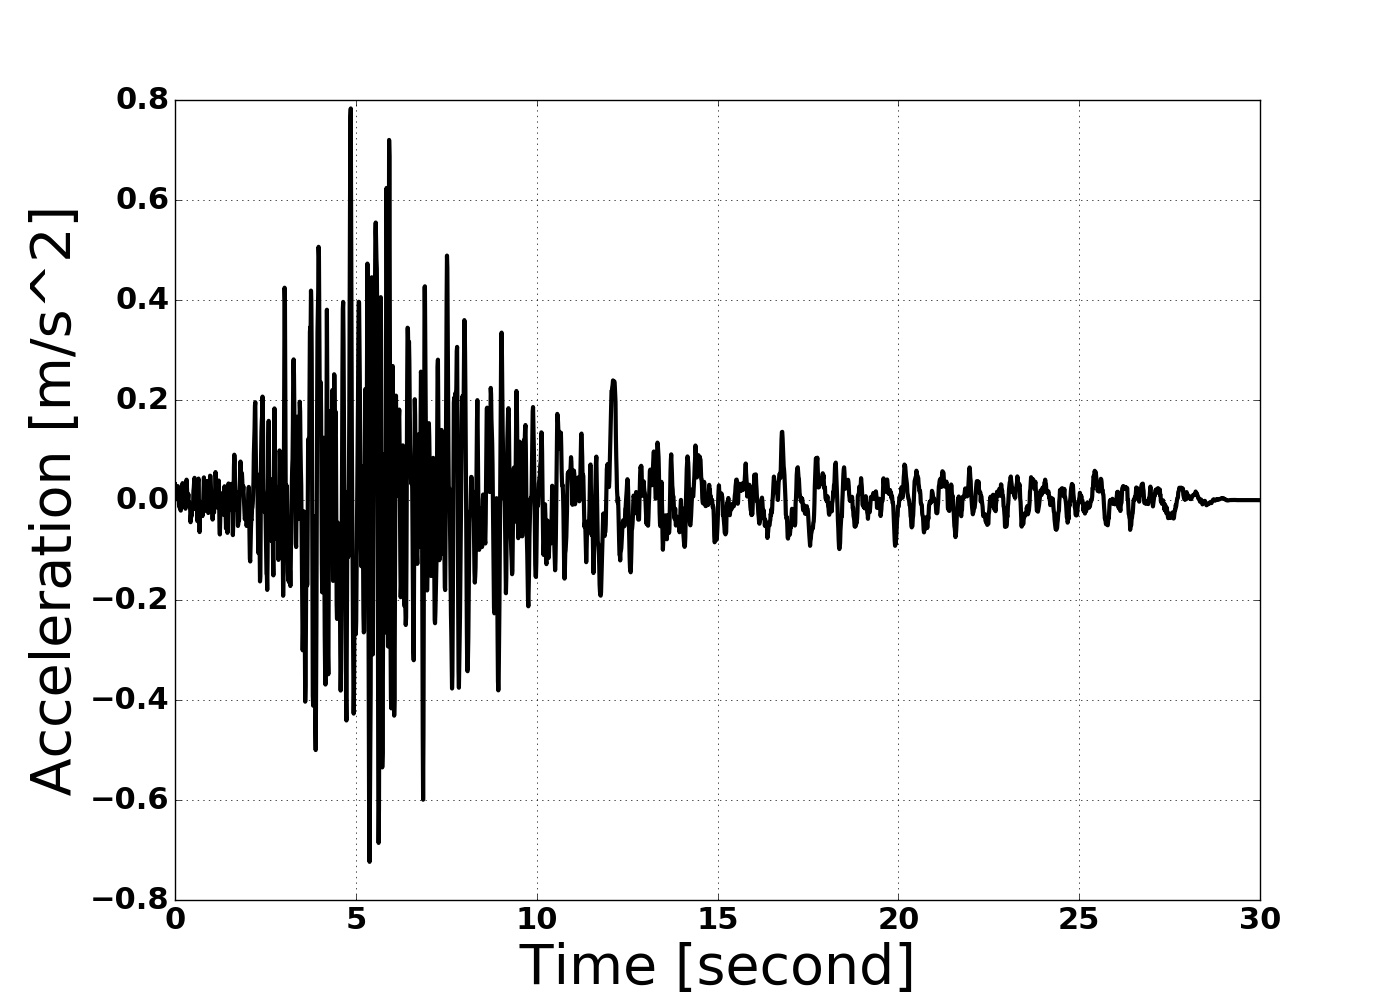
\includegraphics[width = 5cm]{./Figure-files/Day1/Nuclear_Power_Plant_with_3by1D_motions_from_Deconvolution/scaled_NORTHR_y_A.jpg}
  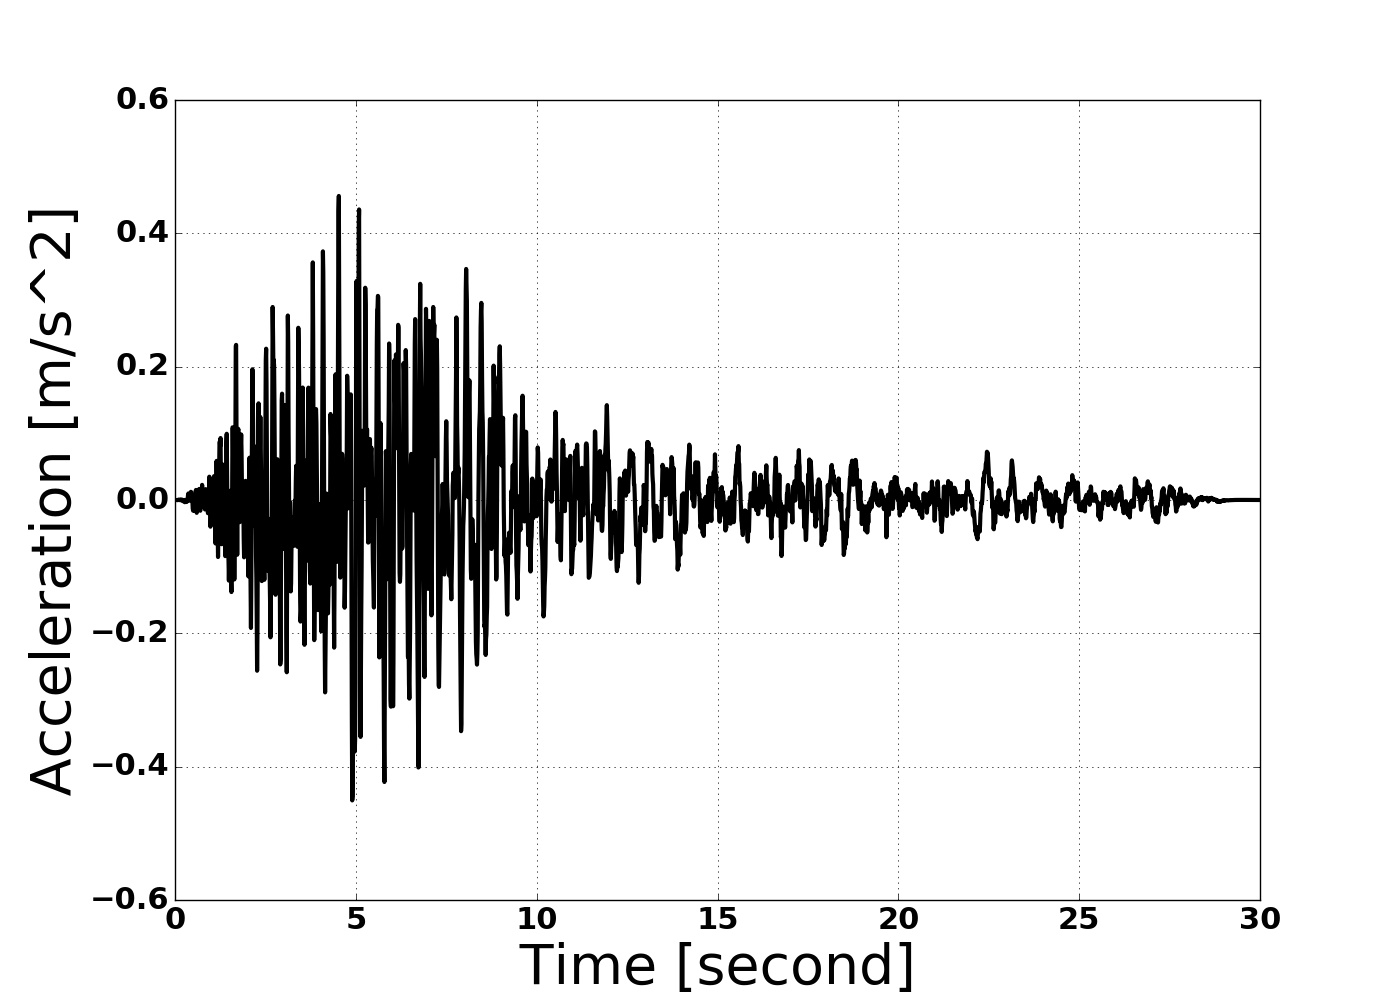
\includegraphics[width = 5cm]{./Figure-files/Day1/Nuclear_Power_Plant_with_3by1D_motions_from_Deconvolution/scaled_NORTHR_z_A.jpg}
  \caption{Acceleration Deconvolution, from left to right in x, y, z directions respectively. }
  \label{fig_motion_deconvolution2}
\end{figure}

\begin{figure}[H]
  \centering
  \includegraphics[width = 5cm]{./Figure-files/Day1/Nuclear_Power_Plant_with_3by1D_motions_from_Deconvolution/scaled_NORTHR_x_D.jpg}
  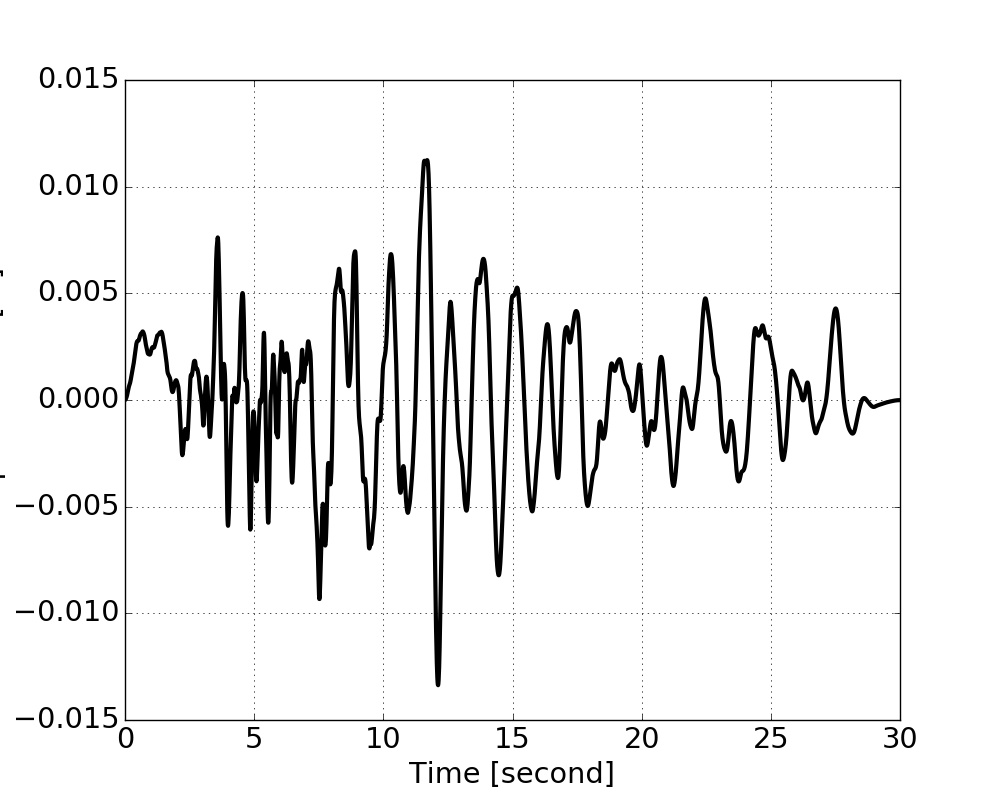
\includegraphics[width = 5cm]{./Figure-files/Day1/Nuclear_Power_Plant_with_3by1D_motions_from_Deconvolution/scaled_NORTHR_y_D.jpg}
  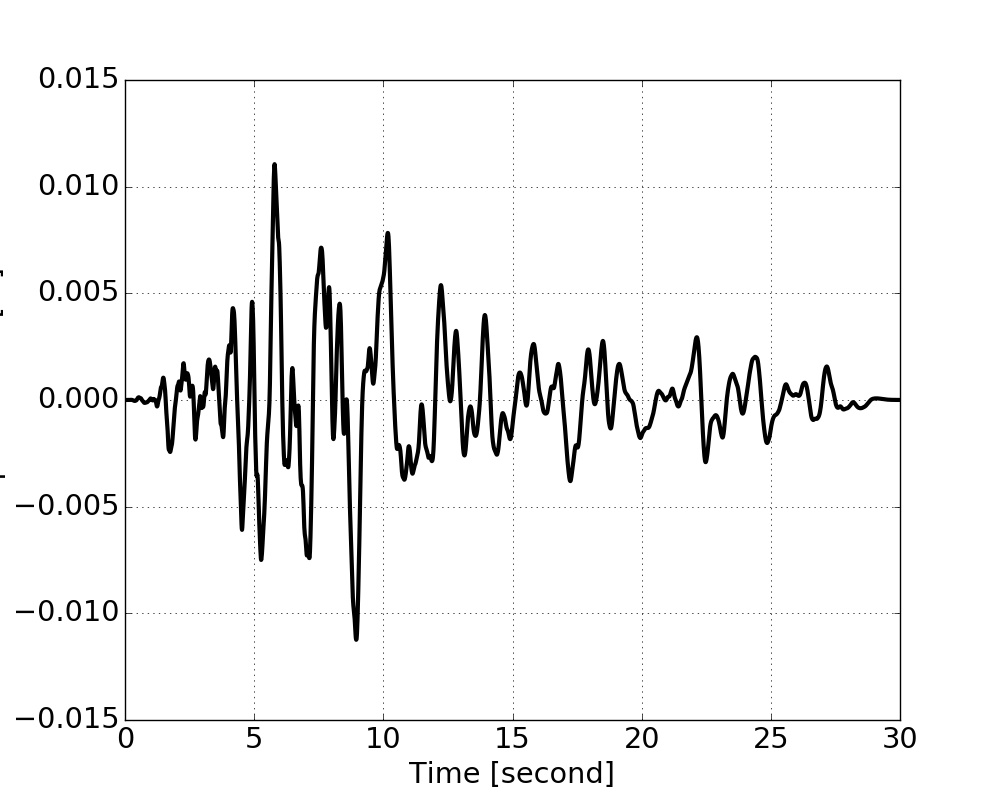
\includegraphics[width = 5cm]{./Figure-files/Day1/Nuclear_Power_Plant_with_3by1D_motions_from_Deconvolution/scaled_NORTHR_z_D.jpg}
  \caption{Displacement Deconvolution, from left to right in x, y, z directions respectively. }
  \label{fig_motion_deconvolution3}
\end{figure}


The Modeling parameters are listed.
\begin{itemize}
  \item Soil 
  \begin{itemize}
    \item Unit weight, $\gamma$, \enspace \enspace 21.4 kPa
    \item Shear velocity, $Vs$, \enspace \enspace 500 m/s
    \item Young's modulus, $E$, \enspace \enspace 1.3 GPa
    \item Poisson's ratio, $\nu$, \enspace \enspace 0.25
    \item Shear strength, $S_u$, \enspace \enspace 650 kPa
    \item von Mises radius, $k$, \enspace \enspace 60 kPa
    \item kinematic hardening, $H_a$, \enspace \enspace 30 MPa
    \item kinematic hardening, $C_r$, \enspace \enspace 25
  \end{itemize}
  \item Structure
  \begin{itemize}
    \item Unit weight, $\gamma$, \enspace \enspace 24 kPa
    \item Young's modulus, $E$, \enspace \enspace 20 GPa
    \item Poisson's ratio, $\nu$, \enspace \enspace 0.21
  \end{itemize}
\end{itemize}

% ******************************************************************
% ******************************************************************
% ******************************************************************
\clearpage
\newpage
\section{Single element Models: illustrate the elastic-plastic behavior}
\label{Single_element_Models_illustrate_the_elastic-plastic_behavior}

The compressed package of Real-ESSI input files for this example with von-Mises material model are available 
\href{http://sokocalo.engr.ucdavis.edu/~jeremic/lecture_notes_online_material/_Chapter_Short_Course_Examples/short-course-examples/Day1/Single_element_Models_illustrate_the_elastic-plastic_behavior/vonMises/_all_files_packaged_for_vonMises.tar.gz}{HERE}. 

The compressed package of Real-ESSI input files for this example with Drucker-Prager material model are available 
\href{http://sokocalo.engr.ucdavis.edu/~jeremic/lecture_notes_online_material/_Chapter_Short_Course_Examples/short-course-examples/Day1/Single_element_Models_illustrate_the_elastic-plastic_behavior/DruckerPrager/_all_files_packaged_for_DruckerPrager.tar.gz}{HERE}. 



The Modeling parameters are listed.
\begin{itemize}
  \item von-Mises linear hardening material model 
  \begin{itemize}
    \item Mass Density, $\rho$, \enspace \enspace 0.0 $kg/m^3$
    \item Young's modulus, $E$, \enspace \enspace 20 MPa
    \item Poisson's ratio, $\nu$, \enspace \enspace 0.0
    \item von Mises radius, $k$, \enspace \enspace 100 kPa
    \item kinematic hardening rate, $K_{kine} $, \enspace \enspace 2 MPa
    \item isotropic hardening rate, $K_{iso} $, \enspace \enspace 0 Pa
  \end{itemize}
  \item Drucker-Prager nonlinear hardening material model 
  \begin{itemize}
    \item Mass Density, $\rho$, \enspace \enspace 0.0 $kg/m^3$
    \item Young's modulus, $E$, \enspace \enspace 20 MPa
    \item Poisson's ratio, $\nu$, \enspace \enspace 0.0
    \item Drucker-Prager, $k$, \enspace \enspace 0.179527
    \item nonlinear kinematic hardening, $H_a$, \enspace \enspace 20 MPa
    \item nonlinear kinematic hardening, $C_r$, \enspace \enspace 100
    \item isotropic hardening rate, $K_{iso} $, \enspace \enspace 0 Pa
    \item initial confining stress, $p_0$, \enspace \enspace 1 Pa
  \end{itemize}
\end{itemize}


\begin{figure}[H]
  \centering
  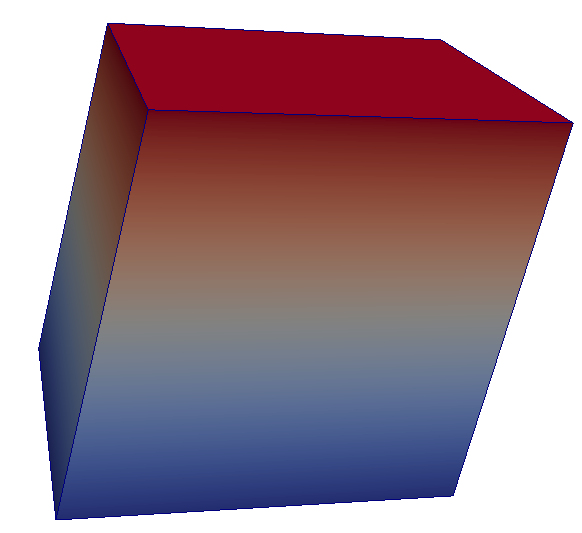
\includegraphics[width = 6cm]{./Figure-files/Day1/Single_element_Models_illustrate_the_elastic-plastic_behavior/overview.png}
  \caption{Simulation Model of Single Element}
  \label{fig_single_element_elastic-plastic}
\end{figure}

The illustrative nonlinear material behavior is shown in Fig.~\ref{fig_day1_illustration_nonlinear_single_element}.

\begin{figure}[H]
  \centering
  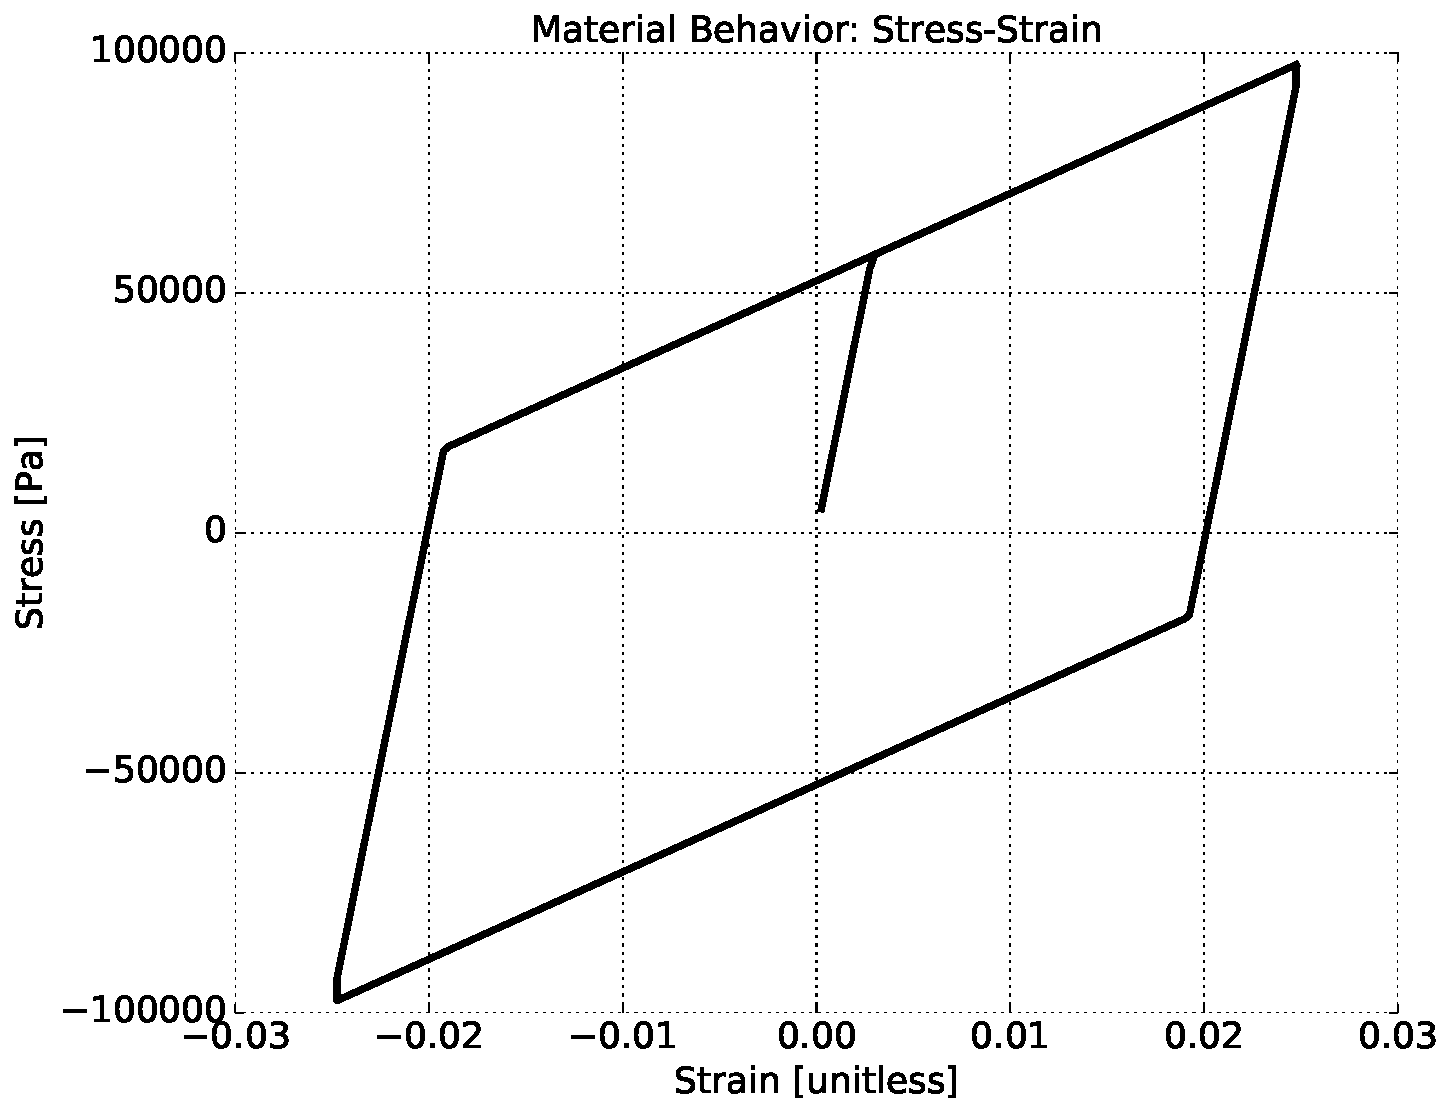
\includegraphics[width = 7cm]{./Figure-files/Day1/Single_element_Models_illustrate_the_elastic-plastic_behavior/vonMises.pdf}
  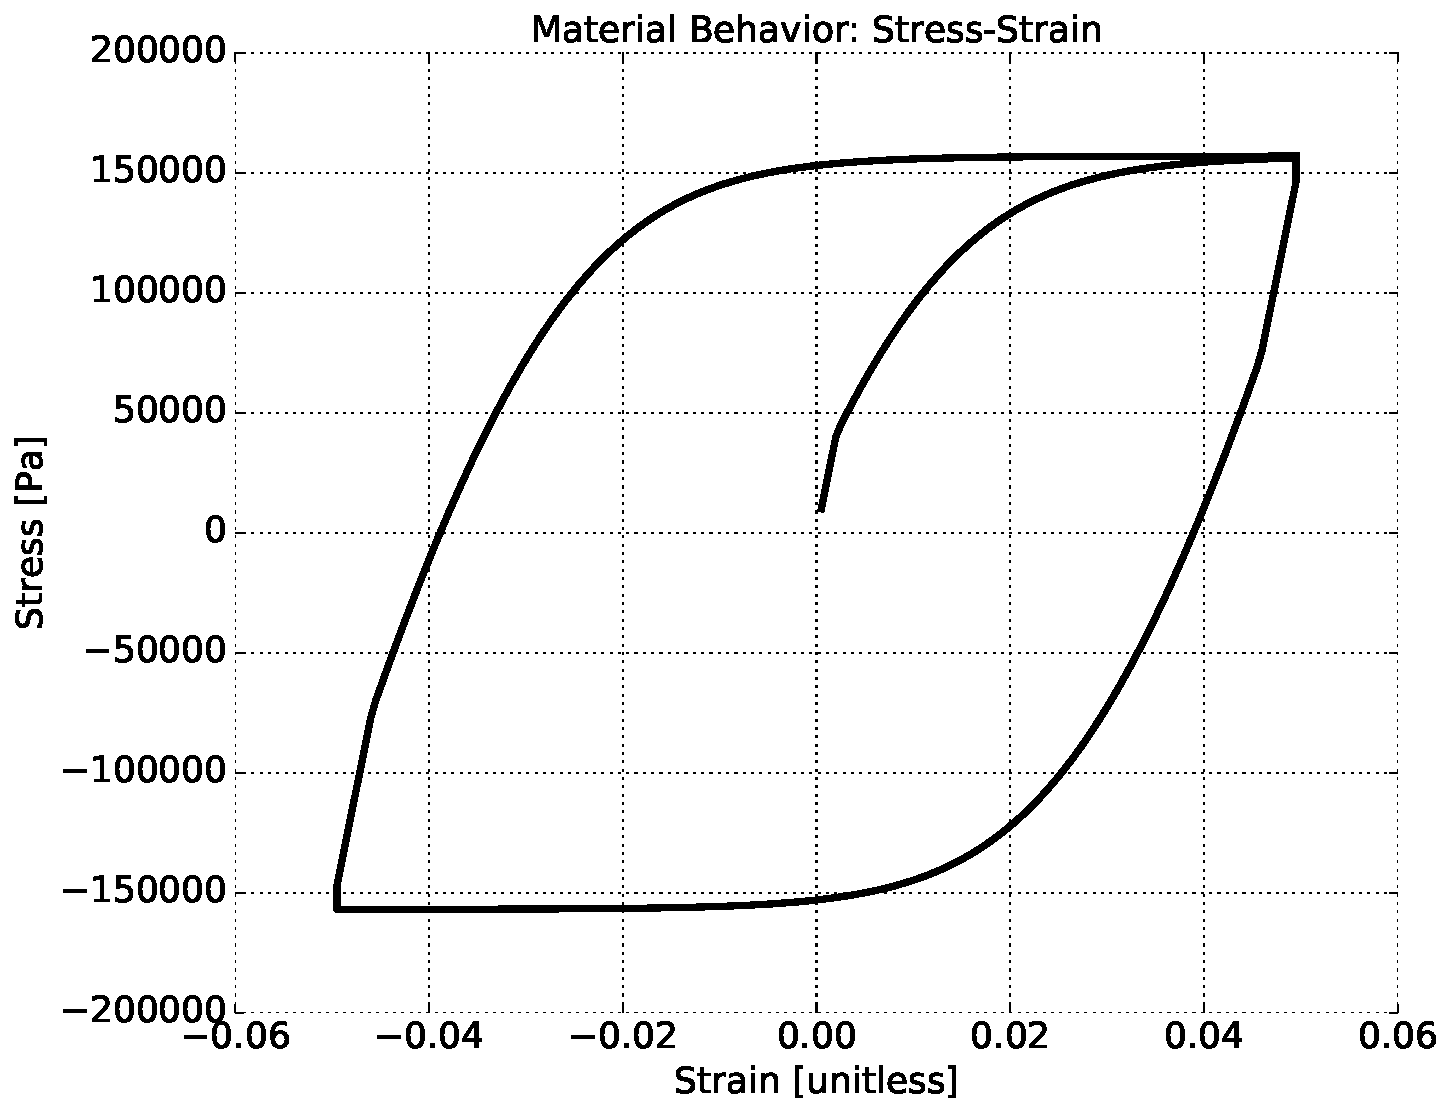
\includegraphics[width = 7cm]{./Figure-files/Day1/Single_element_Models_illustrate_the_elastic-plastic_behavior/DruckerPrager.pdf}
  \caption{ Illustration of Nonlinear Material Behavior }
  \label{fig_day1_illustration_nonlinear_single_element}
\end{figure}



% ******************************************************************
% ******************************************************************
% ******************************************************************
\clearpage
\newpage
\section{Pushover for Nonlinear Frame}
\label{Pushover_for_Nonlinear_Frame}


The Real-ESSI input files for this example are available 
\href{http://sokocalo.engr.ucdavis.edu/~jeremic/lecture_notes_online_material/_Chapter_Short_Course_Examples/short-course-examples/Day1/Pushover_for_Nonlinear_Frame}{HERE}. 
The compressed package of Real-ESSI input files for this example is available 
\href{http://sokocalo.engr.ucdavis.edu/~jeremic/lecture_notes_online_material/_Chapter_Short_Course_Examples/short-course-examples/Day1/Pushover_for_Nonlinear_Frame/_all_files_packaged_for_Pushover_for_Nonlinear_Frame.tar.gz}{HERE}. 

\begin{figure}[H]
  \centering
  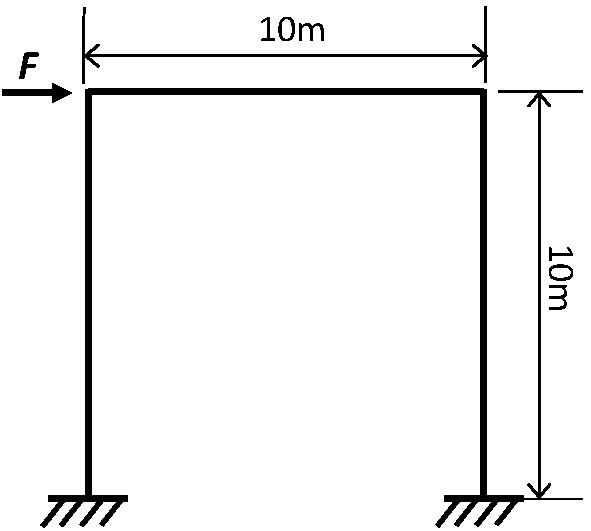
\includegraphics[width = 6cm]{./Figure-files/Day1/Pushover_for_Nonlinear_Frame/overview.pdf}
  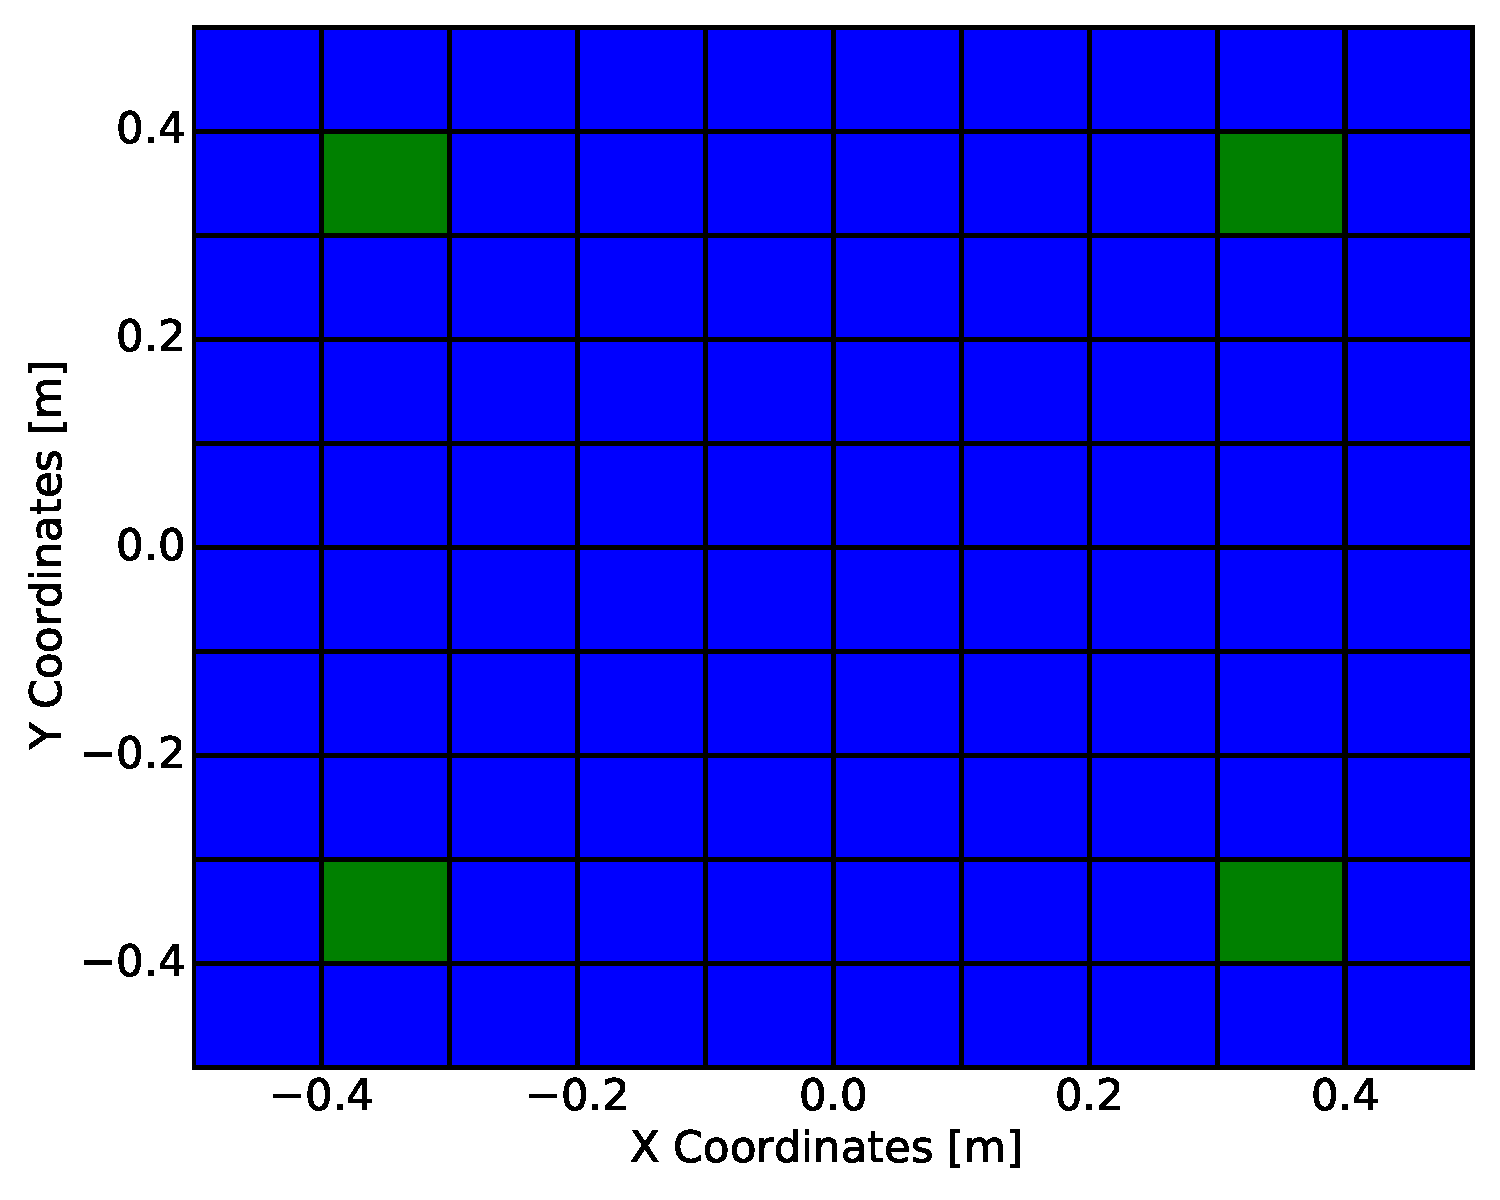
\includegraphics[width = 6cm]{./Figure-files/Day1/Pushover_for_Nonlinear_Frame/rectangle_rebar2.pdf}
  \caption{Model of Pushover Simulation and the Cross Section of Fiber Beam (Concrete and Rebar) }
  \label{fig_single_element_pushover}
\end{figure}

The illustrative result is shown in Fig.~\ref{fig_day1_fiberbeam_pushover_results}.
\begin{figure}[H]
  \centering
  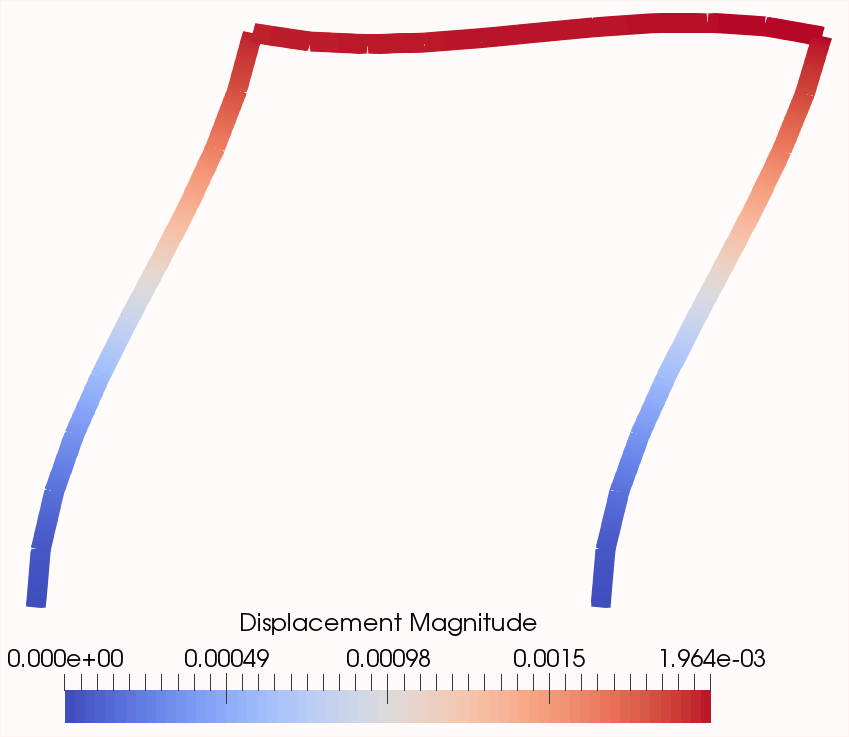
\includegraphics[width = 8cm]{./Figure-files/Day1/Pushover_for_Nonlinear_Frame/fiberBeamDeform.png}
  \caption{Illustration results of Fiber Pushover}
  \label{fig_day1_fiberbeam_pushover_results}
\end{figure}


\begin{figure}[H]
  \centering
  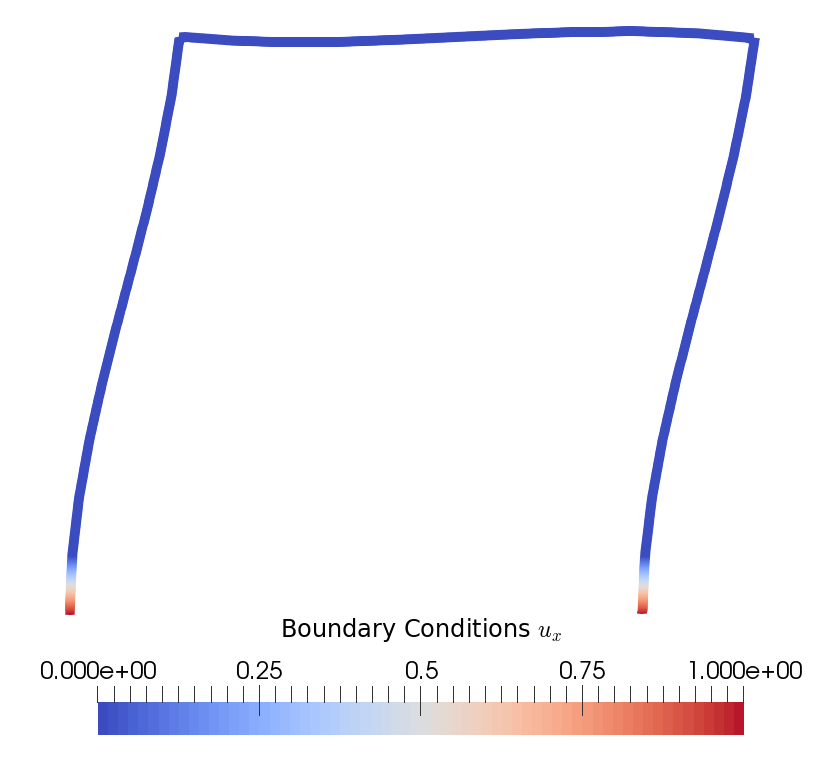
\includegraphics[width = 8cm]{./Figure-files/Day1/Pushover_for_Nonlinear_Frame/boundary_condition_frame.png}
  \caption{Boundary Condition $u_x$ of Fiber Pushover}
  \label{fig_day1_fiberbeam_pushover_results_bc}
\end{figure}

The Modeling parameters are listed.
\begin{itemize}
  \item Uniaxial concrete 
  \begin{itemize}
    \item Compressive strength,  \enspace \enspace 24 MPa
    \item Strain at compressive strength,  \enspace \enspace 0.001752
    \item Crushing strength,  \enspace \enspace 0.0 Pa
    \item Strain at compressive strength,  \enspace \enspace 0.003168
    \item lambda, \enspace \enspace 0.5
    \item Tensile strength, \enspace \enspace 0 Pa
    \item Tension softening stiffness, \enspace \enspace 0 Pa
  \end{itemize}
  \item Uniaxial steel
  \begin{itemize}
    \item Yield strength, \enspace \enspace 413.8 MPa
    \item Young's modulus, \enspace \enspace 200 GPa
    \item Strain hardening ratio, \enspace \enspace 0.01
    \item R0, \enspace \enspace 18.0
    \item cR1,  \enspace \enspace 0.925
    \item cR2,  \enspace \enspace 0.15
    \item a1, \enspace \enspace 0.0
    \item a2, \enspace \enspace 55.0
    \item a3, \enspace \enspace 0.0
    \item a4, \enspace \enspace 55.0
  \end{itemize}
\end{itemize}


% ******************************************************************
% ******************************************************************
% ******************************************************************
\clearpage
\newpage
\section{Preprocess examples with Gmsh}
\label{Preprocess_examples_with_Gmsh}
\subsection{Cantilever Example}


The Real-ESSI input files for this example are available 
\href{http://sokocalo.engr.ucdavis.edu/~jeremic/lecture_notes_online_material/_Chapter_Short_Course_Examples/short-course-examples/Day1/Preprocess_examples_with_Gmsh/cantilever}{HERE}. 
The compressed package of Real-ESSI input files for this example is available 
\href{http://sokocalo.engr.ucdavis.edu/~jeremic/lecture_notes_online_material/_Chapter_Short_Course_Examples/short-course-examples/Day1/Preprocess_examples_with_Gmsh/cantilever/_all_files_packaged_for_cantilever.tar.gz}{HERE}. 


\begin{figure}[H]
  \centering
  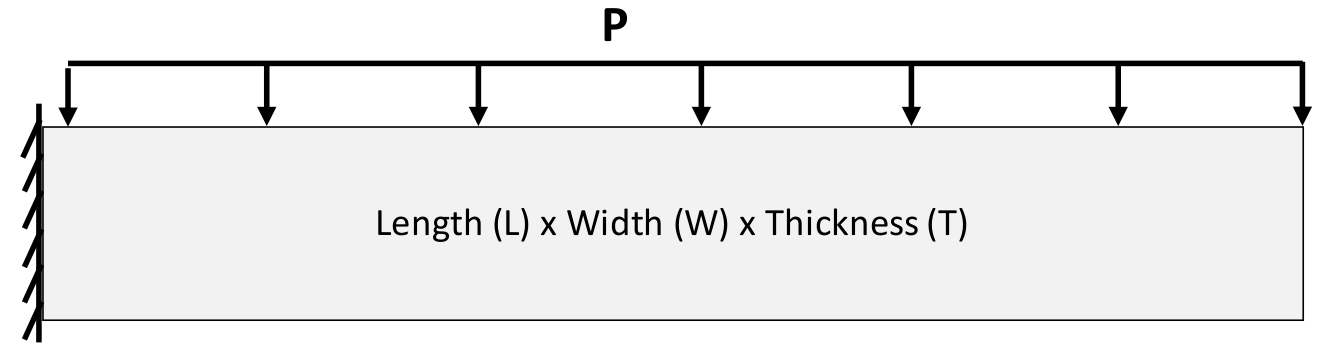
\includegraphics[width = 10cm]{./Figure-files/Day1/Preprocess_examples_with_Gmsh/example1/overview.png}
  \caption{Simulation Model Cantilever}
  \label{fig_gmsh_ex1}
\end{figure}


The illustration results is shown in Fig.~\ref{fig_day1_gmsh_ex_cantilever_results}.

\begin{figure}[H]
  \centering
  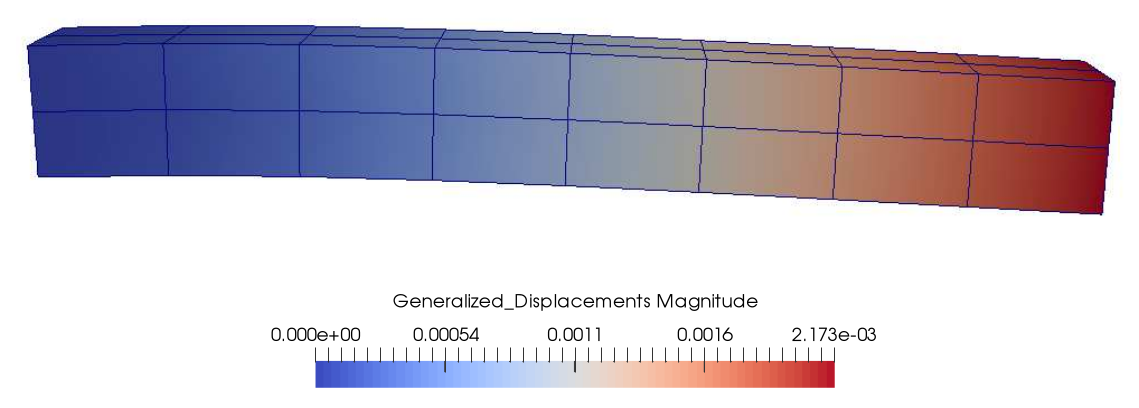
\includegraphics[width = 10cm]{./Figure-files/Day1/Preprocess_examples_with_Gmsh/example1/cantilever_results.png}
  \caption{Simulation Model Cantilever Illustration Results }
  \label{fig_day1_gmsh_ex_cantilever_results}
\end{figure}




% ******************************************************************
% ******************************************************************
\clearpage
\newpage
\subsection{Brick-shell-beam Example}

The Real-ESSI input files for this example are available 
\href{http://sokocalo.engr.ucdavis.edu/~jeremic/lecture_notes_online_material/_Chapter_Short_Course_Examples/short-course-examples/Day1/Preprocess_examples_with_Gmsh/brick-shell-beam}{HERE}. 
The compressed package of Real-ESSI input files for this example is available 
\href{http://sokocalo.engr.ucdavis.edu/~jeremic/lecture_notes_online_material/_Chapter_Short_Course_Examples/short-course-examples/Day1/Preprocess_examples_with_Gmsh/brick-shell-beam/_all_files_packaged_for_brick-shell-beam.tar.gz}{HERE}. 



\begin{figure}[H]
  \centering
  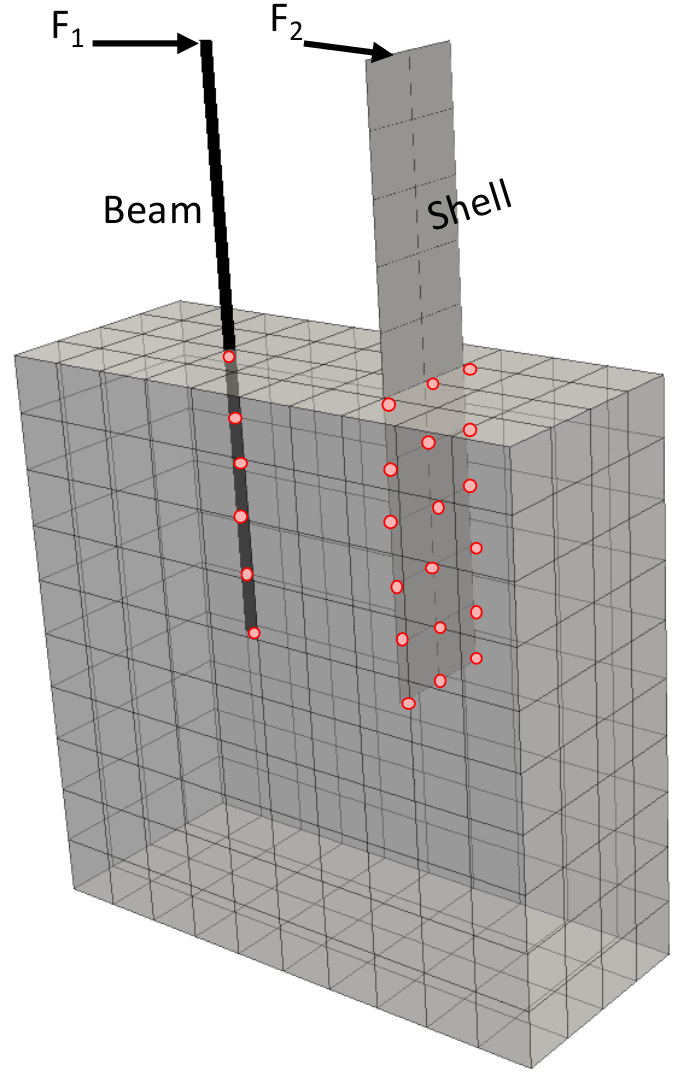
\includegraphics[width = 5cm]{./Figure-files/Day1/Preprocess_examples_with_Gmsh/example2/overview.png}
  \caption{Simulation Model Brick-Shell-Beam}
  \label{fig_gmsh_ex2}
\end{figure}


The illustration results is shown in Fig.~\ref{fig_day1_gmsh_ex_beam_shell_brick}.

\begin{figure}[H]
  \centering
  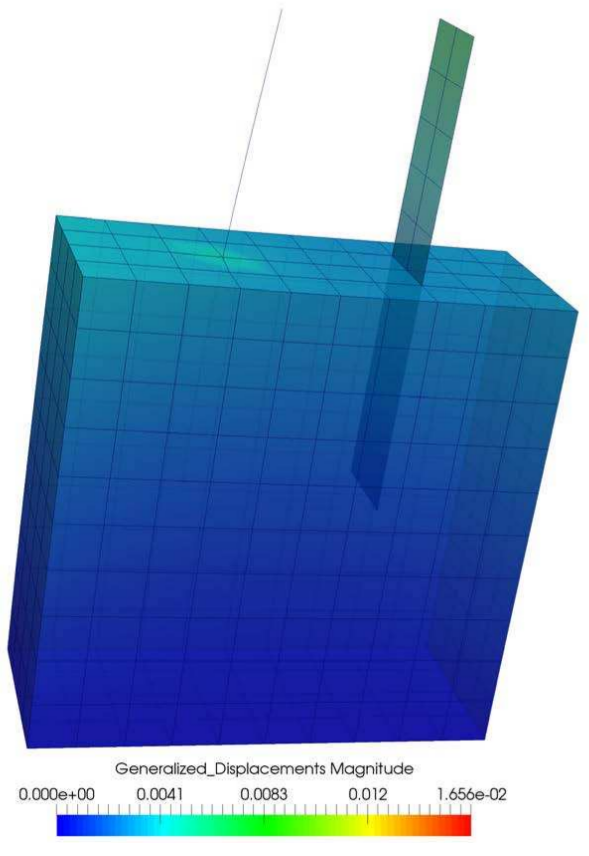
\includegraphics[width = 6cm]{./Figure-files/Day1/Preprocess_examples_with_Gmsh/example2/beam-shell-results-visual.png}
  \caption{Brick-Shell-Beam Illustration Results }
  \label{fig_day1_gmsh_ex_beam_shell_brick}
\end{figure}


% ******************************************************************
% ******************************************************************
\clearpage
\newpage
\subsection{DRM 2D Example}

The Real-ESSI input files for this example are available 
\href{http://sokocalo.engr.ucdavis.edu/~jeremic/lecture_notes_online_material/_Chapter_Short_Course_Examples/short-course-examples/Day1/Preprocess_examples_with_Gmsh/DRM2D}{HERE}. 
The compressed package of Real-ESSI input files for this example is available 
\href{http://sokocalo.engr.ucdavis.edu/~jeremic/lecture_notes_online_material/_Chapter_Short_Course_Examples/short-course-examples/Day1/Preprocess_examples_with_Gmsh/DRM2D/_all_files_packaged_for_DRM2D.tar.gz}{HERE}. 

\begin{figure}[H]
  \centering
  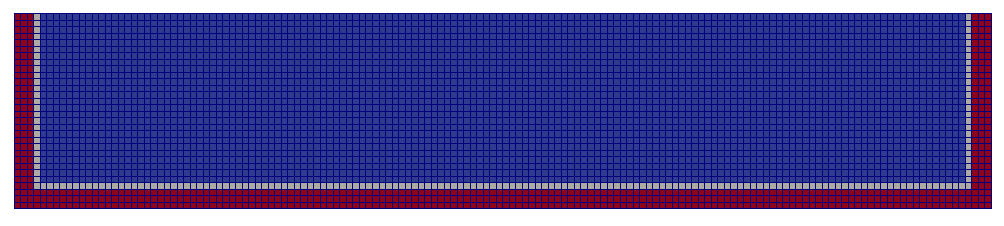
\includegraphics[width = 10cm]{./Figure-files/Day1/Preprocess_examples_with_Gmsh/example3/overview.png}
  \caption{Simulation Model DRM 2D}
  \label{fig_gmsh_ex3}
\end{figure}

The illustration results of free field DRM 2D Model under 1D motion is shown 
in Fig.~\ref{fig_day1_DRM2D_results}. 

\begin{figure}[H]
  \centering
  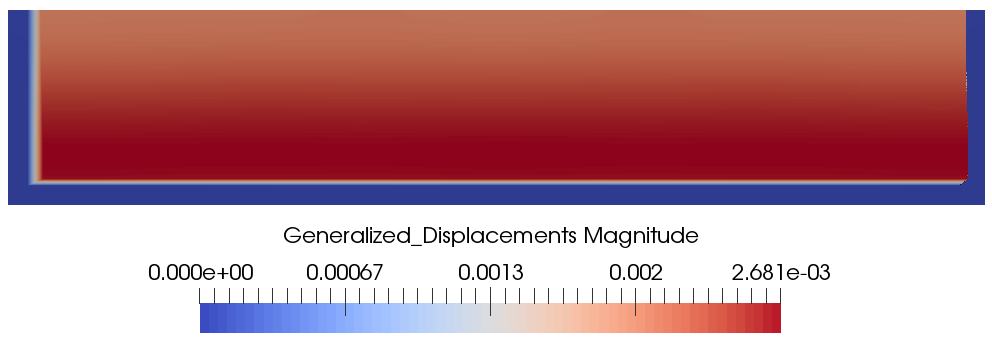
\includegraphics[width = 10cm]{./Figure-files/Day1/Preprocess_examples_with_Gmsh/example3/DRM2D_results.png}
  \caption{Simulation Model DRM 2D}
  \label{fig_day1_DRM2D_results}
\end{figure}

% ******************************************************************
% ******************************************************************
\clearpage
\newpage
\subsection{DRM 3D Example}


The Real-ESSI input files for this example are available 
\href{http://sokocalo.engr.ucdavis.edu/~jeremic/lecture_notes_online_material/_Chapter_Short_Course_Examples/short-course-examples/Day1/Preprocess_examples_with_Gmsh/DRM3D}{HERE}. 
The compressed package of Real-ESSI input files for this example is available 
\href{http://sokocalo.engr.ucdavis.edu/~jeremic/lecture_notes_online_material/_Chapter_Short_Course_Examples/short-course-examples/Day1/Preprocess_examples_with_Gmsh/DRM3D/_all_files_packaged_for_DRM3D.tar.gz}{HERE}. 

\begin{figure}[H]
  \centering
  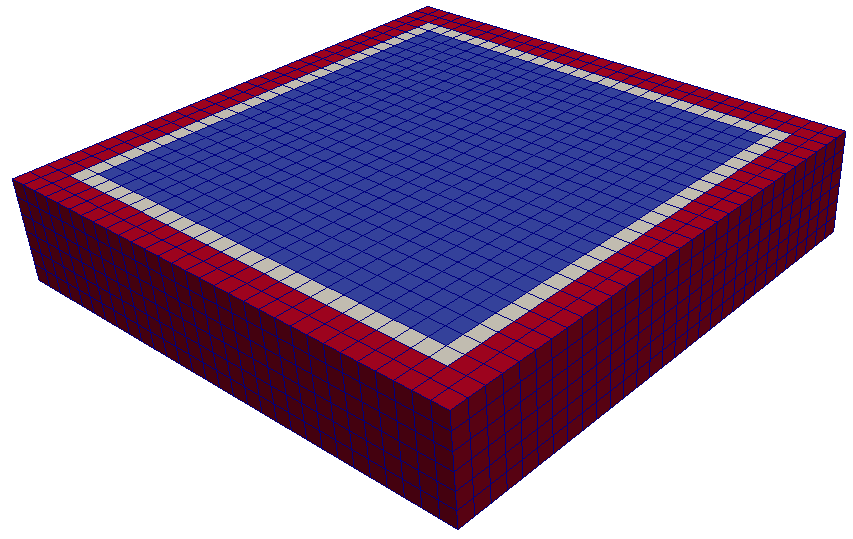
\includegraphics[width = 10cm]{./Figure-files/Day1/Preprocess_examples_with_Gmsh/example4/overview.png}
  \caption{Simulation Model DRM 3D}
  \label{fig_gmsh_ex4}
\end{figure}

The illustration results of free field DRM 3D Model under 1D motion is shown 
in Fig.~\ref{fig_day1_DRM3D_results}. 

\begin{figure}[H]
  \centering
  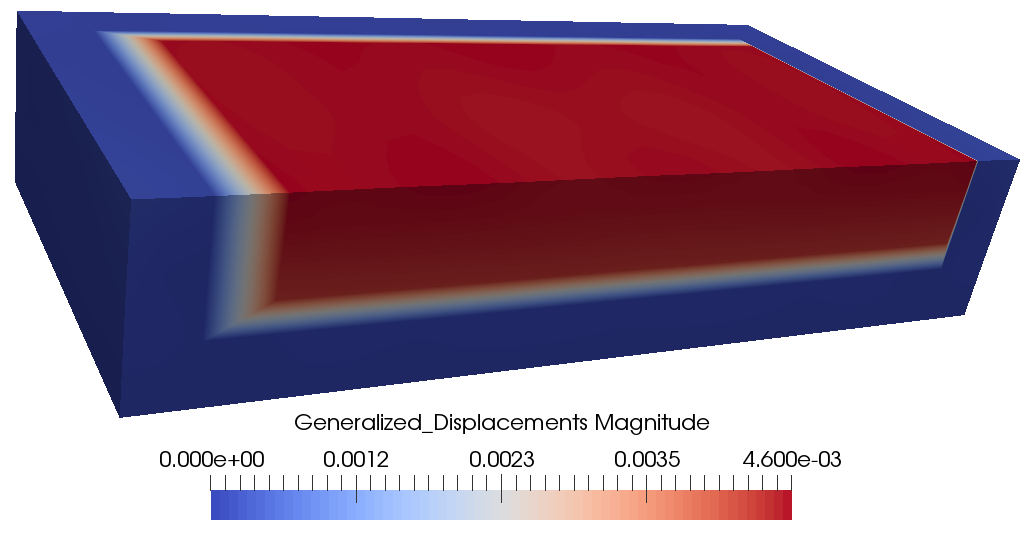
\includegraphics[width = 10cm]{./Figure-files/Day1/Preprocess_examples_with_Gmsh/example4/DRM3D_results.png}
  \caption{Simulation Model DRM 2D}
  \label{fig_day1_DRM3D_results}
\end{figure}


% ******************************************************************
% ******************************************************************
% ******************************************************************
\clearpage
\newpage
\section{Postprocess examples with Paraview}
\label{Postprocess_examples_with_Paraview}
\subsection{Slice Visualization}

The Real-ESSI input files for this example are available 
\href{http://sokocalo.engr.ucdavis.edu/~jeremic/lecture_notes_online_material/_Chapter_Short_Course_Examples/short-course-examples/Day1/Nuclear_Power_Plant_with_1D_motions_from_Deconvolution}{HERE}. 
The compressed package of Real-ESSI input files for this example is available 
\href{http://sokocalo.engr.ucdavis.edu/~jeremic/lecture_notes_online_material/_Chapter_Short_Course_Examples/short-course-examples/Day1/Nuclear_Power_Plant_with_1D_motions_from_Deconvolution/_all_files_packaged_for_Nuclear_Power_Plant_with_1D_motions_from_Deconvolution.tar.gz}{HERE}.  

\begin{figure}[H]
  \centering
  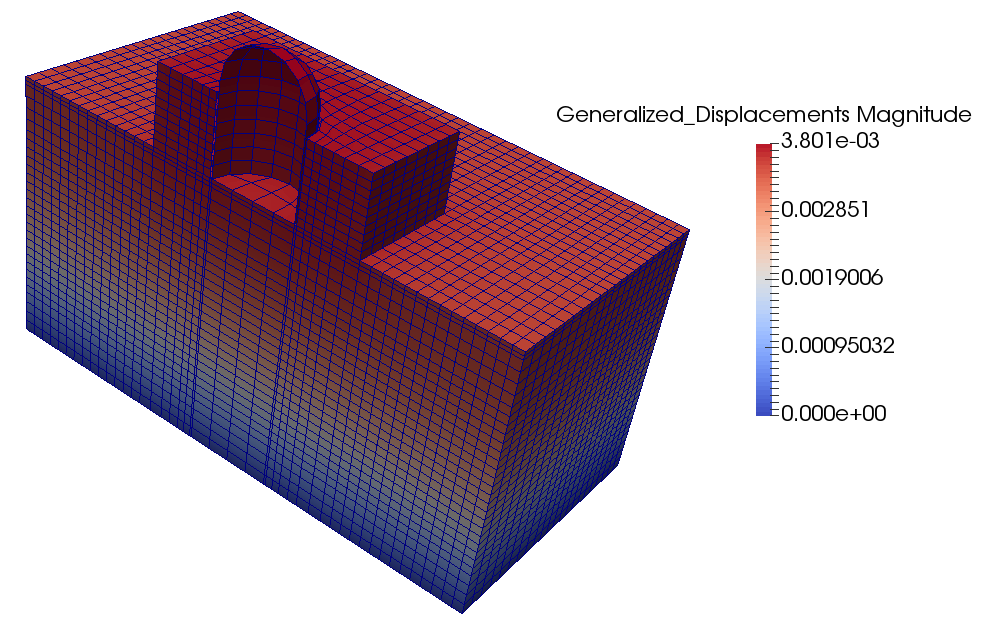
\includegraphics[width = 10cm]{./Figure-files/Day1/Postprocess_examples_with_Paraview/slide_visualization.png}
  \caption{Slice Visualization with Paraview}
  \label{fig_paraview_slice}
\end{figure}


% ******************************************************************
% ******************************************************************
\clearpage
\newpage
\subsection{Stress Visualization}

The Real-ESSI input files for this example are available 
\href{http://sokocalo.engr.ucdavis.edu/~jeremic/lecture_notes_online_material/_Chapter_Short_Course_Examples/short-course-examples/Day1/Nuclear_Power_Plant_with_1D_motions_from_Deconvolution}{HERE}. 
The compressed package of Real-ESSI input files for this example is available 
\href{http://sokocalo.engr.ucdavis.edu/~jeremic/lecture_notes_online_material/_Chapter_Short_Course_Examples/short-course-examples/Day1/Nuclear_Power_Plant_with_1D_motions_from_Deconvolution/_all_files_packaged_for_Nuclear_Power_Plant_with_1D_motions_from_Deconvolution.tar.gz}{HERE}.  

\begin{figure}[H]
  \centering
  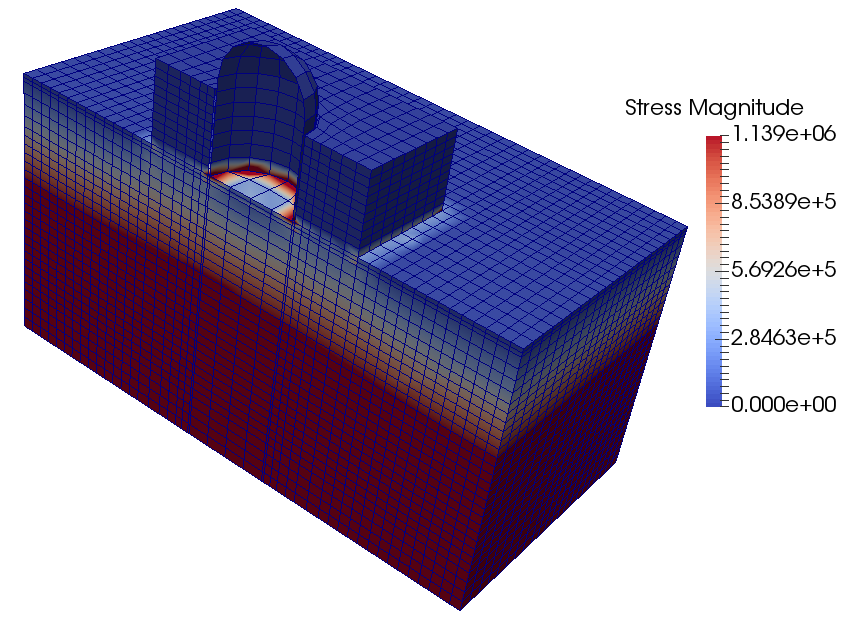
\includegraphics[width = 10cm]{./Figure-files/Day1/Postprocess_examples_with_Paraview/stress_visualization.png}
  \caption{Stress Visualization with Paraview}
  \label{fig_paraview_stress}
\end{figure}

% % ******************************************************************
% % ******************************************************************
% \clearpage
% \newpage
% \subsection{Pore Pressure Visualization in upU Element}

% The Real-ESSI input files for this example are available 
% \href{http://sokocalo.engr.ucdavis.edu/~jeremic/lecture_notes_online_material/_Chapter_Short_Course_Examples/short-course-examples/
% /Day1/Postprocess_examples_with_Paraview/upU}{HERE}. 
% The compressed package of Real-ESSI input files for this example is available 
% \href{http://sokocalo.engr.ucdavis.edu/~jeremic/lecture_notes_online_material/_Chapter_Short_Course_Examples/short-course-examples/
% /Day1/Postprocess_examples_with_Paraview/upU/upU.tar.gz}{HERE}.  

% \begin{figure}[H]
%   \centering
%   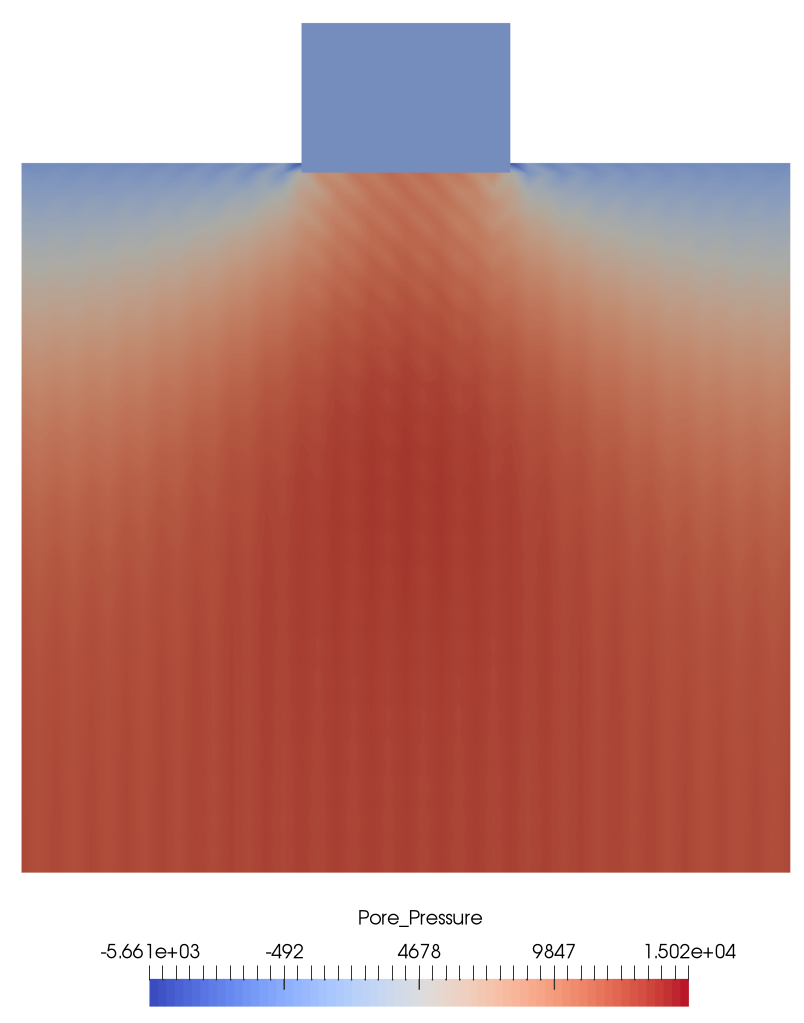
\includegraphics[width = 8cm]{./Figure-files/Day1/Postprocess_examples_with_Paraview/pore_pressure.png}
%   \caption{Pore Pressure Visualization with Paraview}
%   \label{fig_paraview_pore_pressure}
% \end{figure}



% ******************************************************************
% ******************************************************************
\clearpage
\newpage
\subsection{Eigen Visualization}


The Real-ESSI input files for this example are available 
\href{http://sokocalo.engr.ucdavis.edu/~jeremic/lecture_notes_online_material/_Chapter_Short_Course_Examples/short-course-examples/Day1/Postprocess_examples_with_Paraview/eigen}{HERE}. 
The compressed package of Real-ESSI input files for this example is available 
\href{http://sokocalo.engr.ucdavis.edu/~jeremic/lecture_notes_online_material/_Chapter_Short_Course_Examples/short-course-examples/Day1/Postprocess_examples_with_Paraview/eigen/_all_files_packaged_for_eigen.tar.gz}{HERE}.  

\begin{figure}[H]
  \centering
  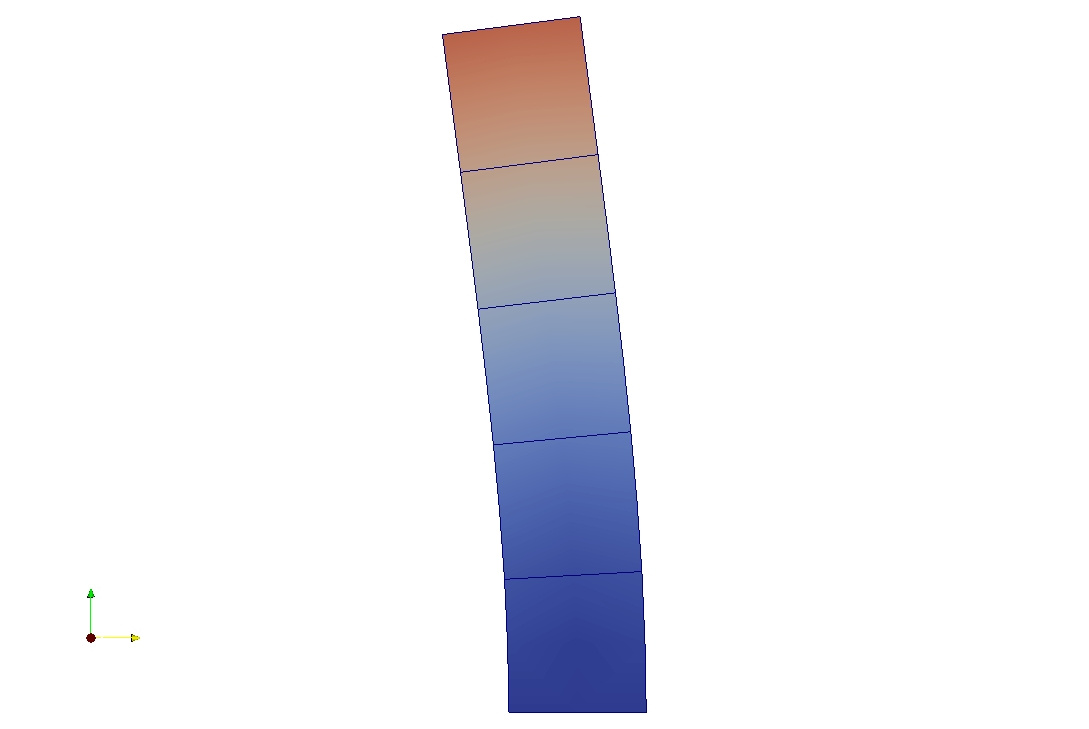
\includegraphics[width = 8cm]{./Figure-files/Day1/Postprocess_examples_with_Paraview/eigenmode1.jpg}
  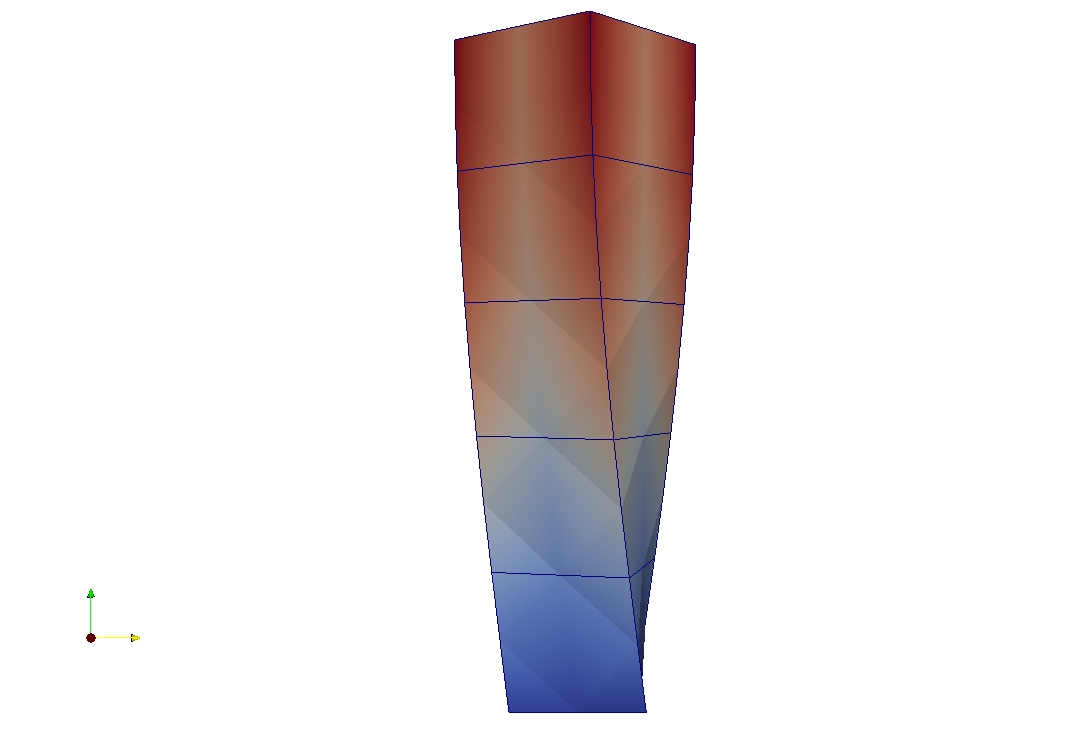
\includegraphics[width = 8cm]{./Figure-files/Day1/Postprocess_examples_with_Paraview/eigenmode2.jpg}
  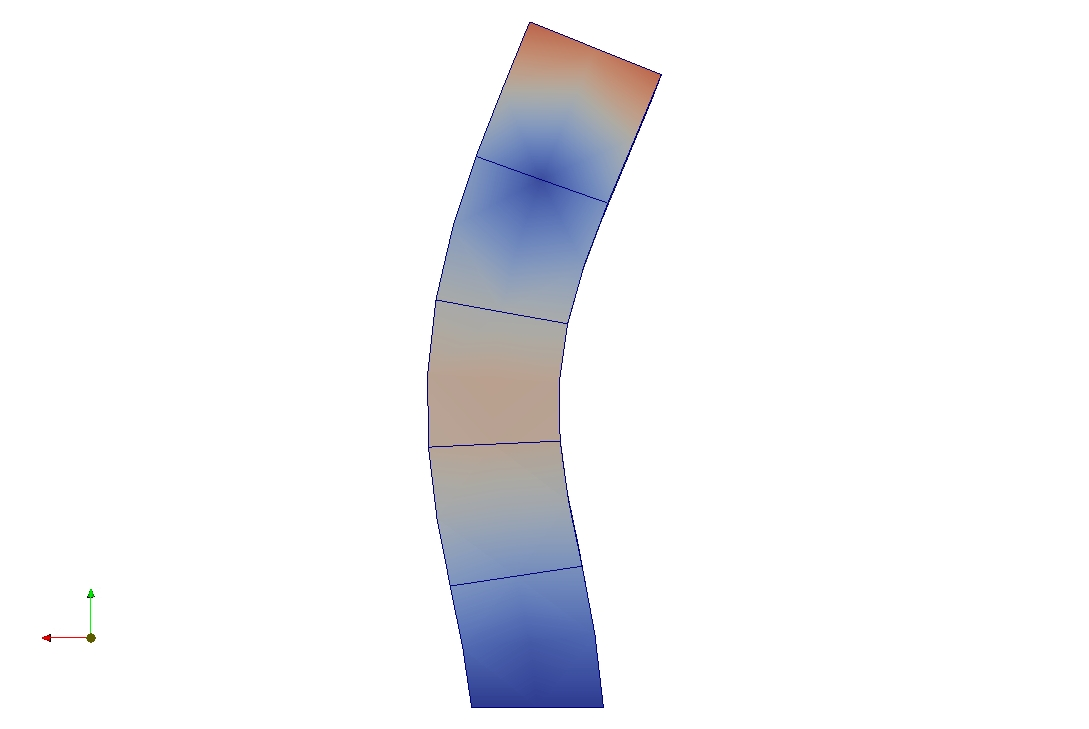
\includegraphics[width = 8cm]{./Figure-files/Day1/Postprocess_examples_with_Paraview/eigenmode3.jpg}
  \caption{Eigen Mode Visualization with Paraview}
  \label{fig_paraview_eigen}
\end{figure}


% ******************************************************************
% ******************************************************************
% ******************************************************************
\clearpage
\newpage
\section{Check Model and Visualization of Boundary Conditions}
\label{Check_Model_and_Visualization_of_Boundary_Conditions}

The Real-ESSI input files for this example are available 
\href{http://sokocalo.engr.ucdavis.edu/~jeremic/lecture_notes_online_material/_Chapter_Short_Course_Examples/short-course-examples/Day1/Check_Model_and_Visualization_of_Boundary_Conditions}{HERE}. 
The compressed package of Real-ESSI input files for this example is available 
\href{http://sokocalo.engr.ucdavis.edu/~jeremic/lecture_notes_online_material/_Chapter_Short_Course_Examples/short-course-examples/Day1/Check_Model_and_Visualization_of_Boundary_Conditions/_all_files_packaged_for_Check_Model_and_Visualization_of_Boundary_Conditions.tar.gz}{HERE}. 

\begin{figure}[H]
  \centering
  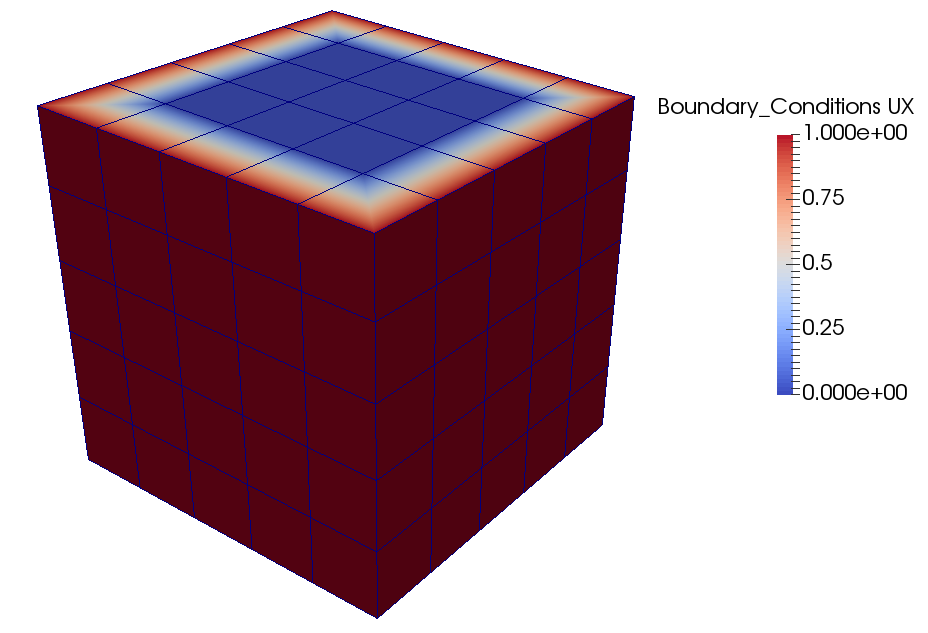
\includegraphics[width = 10cm]{./Figure-files/Day1/Check_Model_and_Visualization_of_Boundary_Conditions/boundary_ux.png}
  \caption{Partition Information Visualization with Paraview}
  \label{fig_check_model_and_boundary_condition_ux}
\end{figure}



\begin{figure}[H]
  \centering
  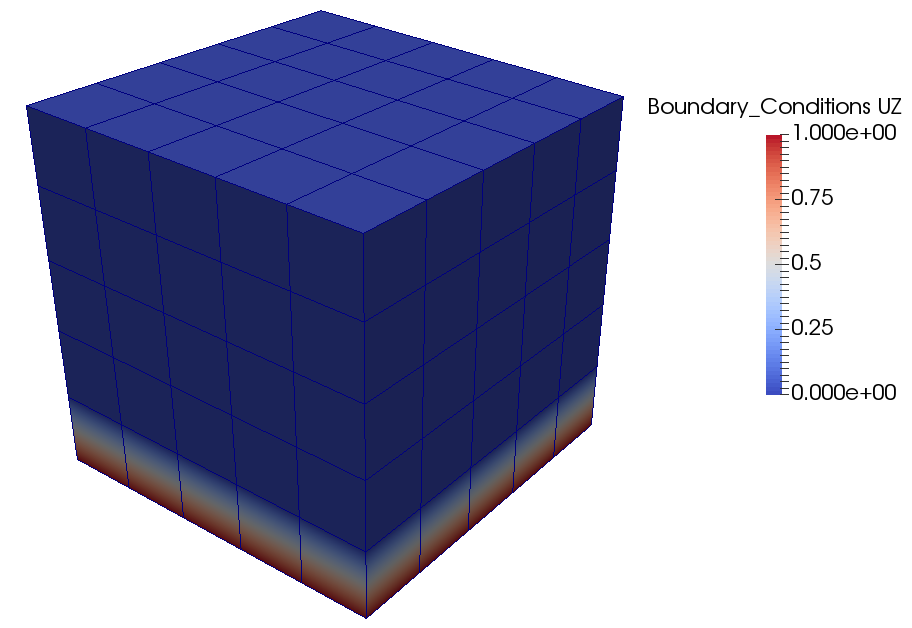
\includegraphics[width = 10cm]{./Figure-files/Day1/Check_Model_and_Visualization_of_Boundary_Conditions/boundary_uz.png}
  \caption{Partition Information Visualization with Paraview}
  \label{fig_check_model_and_boundary_condition_uz}
\end{figure}




% ******************************************************************
% ******************************************************************
% ******************************************************************
\clearpage
\newpage
\section{Restart Simulation}
\label{Restart_Simulation}

\subsection{ Restart in the next stage }

The Real-ESSI input files for this example are available 
\href{http://sokocalo.engr.ucdavis.edu/~jeremic/lecture_notes_online_material/_Chapter_Short_Course_Examples/short-course-examples/Day1/Restart_Simulation/between_stages}{HERE}. 
The compressed package of Real-ESSI input files for this example is available 
\href{http://sokocalo.engr.ucdavis.edu/~jeremic/lecture_notes_online_material/_Chapter_Short_Course_Examples/short-course-examples/Day1/Restart_Simulation/between_stages/_all_files_packaged_for_between_stages.tar.gz}{HERE}. 

\begin{figure}[H]
  \centering
  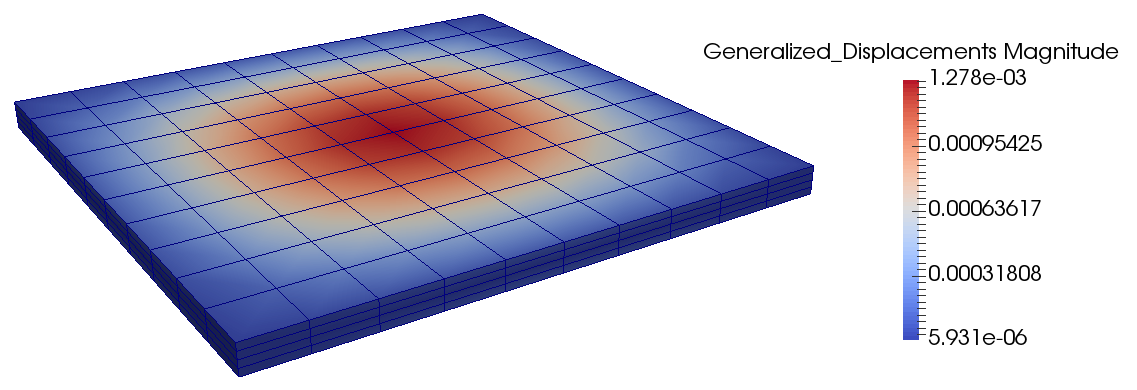
\includegraphics[width = 10cm]{./Figure-files/Day1/Restart_Simulation/restart.png}
  \caption{Restart Simulation}
  \label{fig_restart_simulation1}
\end{figure}

This group of examples illustrate the restart functionality between loading stages. 
There are three test cases in this example.
The two loading stages in the first test case is splitted into two test cases to show the restart feature.
\begin{itemize}
  \item The first test case run through two loading stages.
  \item The second test case only run the first loading stage and saves model state at the end.
  \item The third test case restart the simulation from the saved model state of the second test case. 
      Then, with the restarted model state, the test cases run the second loading stage only. 
\end{itemize}

Finally, the results of the third test case are exactly the same to the first test case.



% ******************************************************************
% ******************************************************************
\clearpage
\newpage
\subsection{ Restart inside the stage }
For the case of inconvergence, restart with the previous loading stage.

The Real-ESSI input files for this example are available 
\href{http://sokocalo.engr.ucdavis.edu/~jeremic/lecture_notes_online_material/_Chapter_Short_Course_Examples/short-course-examples/Day1/Restart_Simulation/in_stage}{HERE}. 
The compressed package of Real-ESSI input files for this example is available 
\href{http://sokocalo.engr.ucdavis.edu/~jeremic/lecture_notes_online_material/_Chapter_Short_Course_Examples/short-course-examples/Day1/Restart_Simulation/in_stage/_all_files_packaged_for_in_stage.tar.gz}{HERE}. 

\begin{figure}[H]
  \centering
  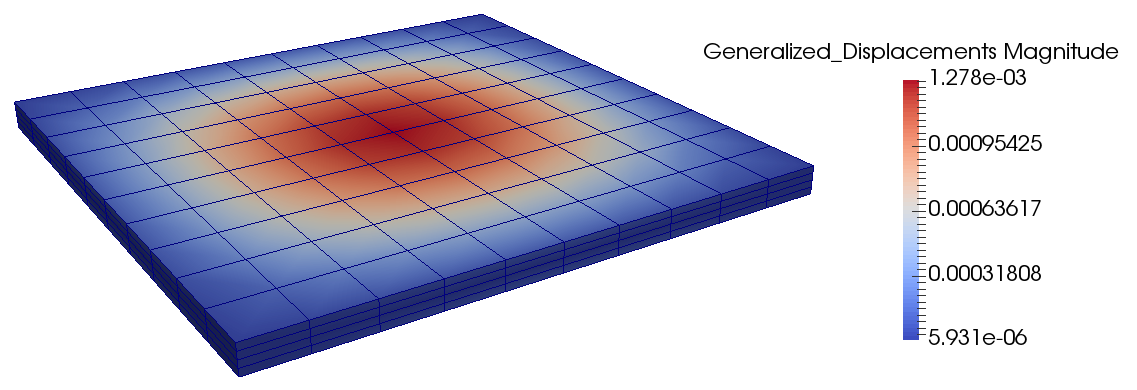
\includegraphics[width = 10cm]{./Figure-files/Day1/Restart_Simulation/restart.png}
  \caption{Restart Simulation}
  \label{fig_restart_simulation2}
\end{figure}


This group of examples illustrate the restart functionality inside one loading stage 
when the simulation cannot converge in the nonlinear analysis.
The nonlinear material model, von-Mises Armstrong-Frederick, is used in all test cases.

There are three test cases in this example.
\begin{itemize}
  \item The first test case run through the whole simulation with a relatively big tolerance of the unbalanced force.
  \item The second test case failed in the middle of the simulation with a relatively small tolerance of the unbalanced force.
      When the second test failed, the model reverted to the last commit model state and saved model state.
  \item The third test case load the saved model state, increased the tolerance of the unbalanced force, and added the 
      remaining load to the model to continue the simulation.
\end{itemize}

Finally, the results of the third test case are exactly the same to the first test case.

Note that in the third test case only the remaining load should be added to the model. 
Whenever the new loading stage is used, the previous loading are all finished,
which means that the static loading becomes constant and the dynamic loading vanishes.






\chapter{Day 2 Motions}
\label{ch-day2}




% ******************************************************************
% ******************************************************************
% ******************************************************************
\clearpage
\newpage
\section{Deconvolution 1D Motions}
\label{Deconvolution_1D_Motions}


\subsection{Free field 1D model, deconvolution 1D motion, model with DRM}
\label{Free_fields_1D_model_with_DRM1}


The Real-ESSI input files for this example are available 
\href{http://sokocalo.engr.ucdavis.edu/~jeremic/lecture_notes_online_material/_Chapter_Short_Course_Examples/Day2/Deconvolution_1D_Motions/Free_fields_1D_model_with_DRM}{HERE}. 
The compressed package of Real-ESSI input files for this example is available 
\href{http://sokocalo.engr.ucdavis.edu/~jeremic/lecture_notes_online_material/_Chapter_Short_Course_Examples/Day2/Deconvolution_1D_Motions/Free_fields_1D_model_with_DRM/_all_files_packaged_for_Free_fields_1D_model_with_DRM.tar.gz}{HERE}. 

The Modeling parameters are listed.
\begin{itemize}
  \item Elastic Material Properties 
  \begin{itemize}
    \item Mass density, $\rho$, \enspace \enspace 2000 $kg/m^3$
    \item Shear Wave Velocity, $V_s$, \enspace \enspace 500 $m/s$
    \item Young's modulus, $E$, \enspace \enspace 1.1 GPa
    \item Poisson's ratio, $\nu$, \enspace \enspace 0.1
  \end{itemize}
\end{itemize}


\begin{figure}[H]
  \centering
  \includegraphics[width = 0.8cm]{./Figure-files/Day2/Deconvolution_1D_Motions/Free_fields_1D_model_with_DRM/overview.png}
  \caption{Simulation Model}
  \label{fig_decon_1D_motion_1D_model1}
\end{figure}

The illustration results of the simulation is shown in Fig.~\ref{fig_decon_1D_motion_1D_model}.
As shown in the results, outside the DRM layer, there is no outgoing waves. 

\begin{figure}[H]
  \centering
  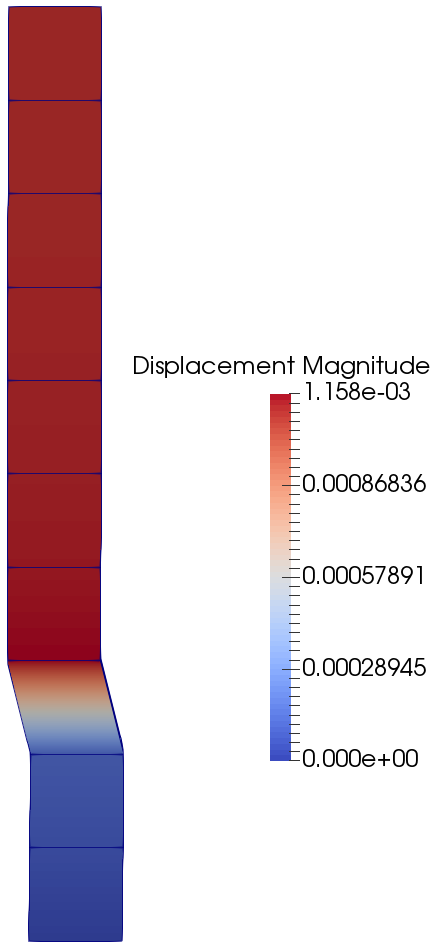
\includegraphics[width = 5cm]{./Figure-files/Day2/Deconvolution_1D_Motions/Free_fields_1D_model_with_DRM/DRM1D_results.png}
  \caption{Simulation Model}
  \label{fig_decon_1D_motion_1D_model_results}
\end{figure}


% ******************************************************************
% ******************************************************************
% ******************************************************************
\clearpage
\newpage
\subsection{Free field 3D model, deconvolution 1D motion, model with DRM}
\label{Free_fields_3D_model_with_DRM1}


The Real-ESSI input files for this example are available 
\href{http://sokocalo.engr.ucdavis.edu/~jeremic/lecture_notes_online_material/_Chapter_Short_Course_Examples/Day2/Deconvolution_1D_Motions/Free_fields_3D_model_with_DRM}{HERE}. 
The compressed package of Real-ESSI input files for this example is available 
\href{http://sokocalo.engr.ucdavis.edu/~jeremic/lecture_notes_online_material/_Chapter_Short_Course_Examples/Day2/Deconvolution_1D_Motions/Free_fields_3D_model_with_DRM/_all_files_packaged_for_Free_fields_3D_model_with_DRM.tar.gz}{HERE}. 

The Modeling parameters are listed.
\begin{itemize}
  \item Elastic Material Properties 
  \begin{itemize}
    \item Mass density, $\rho$, \enspace \enspace 2000 $kg/m^3$
    \item Shear Wave Velocity, $V_s$, \enspace \enspace 500 $m/s$
    \item Young's modulus, $E$, \enspace \enspace 1.1 GPa
    \item Poisson's ratio, $\nu$, \enspace \enspace 0.1
  \end{itemize}
\end{itemize}


\begin{figure}[H]
  \centering
  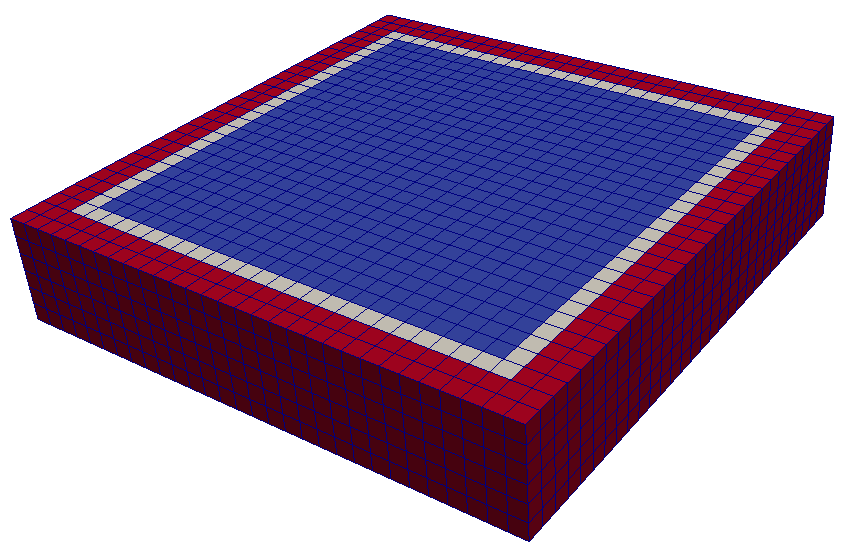
\includegraphics[width = 8cm]{./Figure-files/Day2/Deconvolution_1D_Motions/Free_fields_3D_model_with_DRM/overview.png}
  \caption{Simulation Model}
  \label{fig_decon_1D_motion_3D_model1}
\end{figure}


The illustration results of free field DRM 3D Model under 1D motion is shown 
in Fig.~\ref{fig_day2_DRM3D_results}. 

\begin{figure}[H]
  \centering
  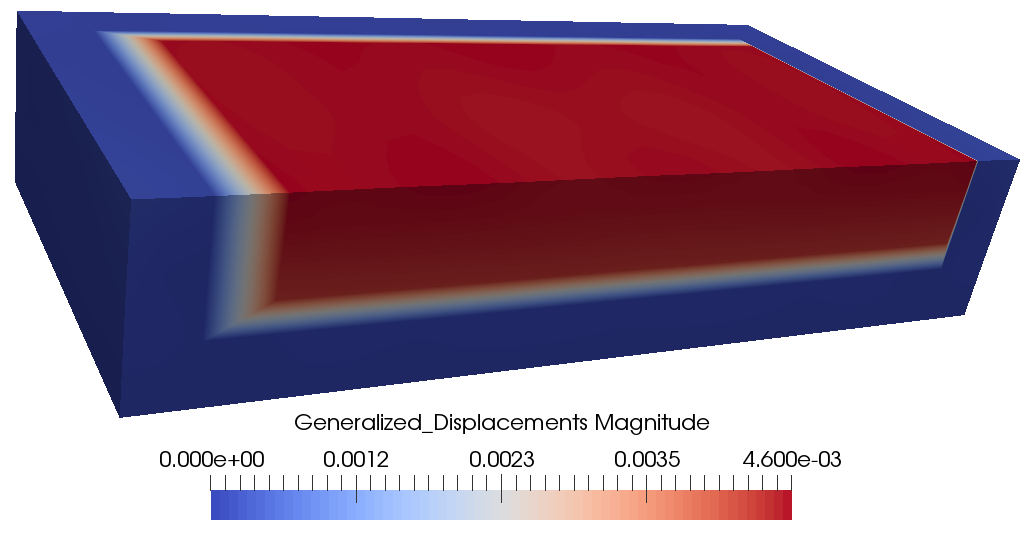
\includegraphics[width = 10cm]{./Figure-files/Day1/Preprocess_examples_with_Gmsh/example4/DRM3D_results.png}
  \caption{Simulation Model DRM 2D}
  \label{fig_day2_DRM3D_results}
\end{figure}



% ******************************************************************
% ******************************************************************
% ******************************************************************
\clearpage
\newpage
\subsection{ESSI 3D building model, deconvolution 1D model, solid model with DRM}
\label{Earthquake_Soil-Structure_Interaction_3D_Model_with_DRM1}

The Real-ESSI input files for this example are available 
\href{http://sokocalo.engr.ucdavis.edu/~jeremic/lecture_notes_online_material/_Chapter_Short_Course_Examples/Day2/Deconvolution_1D_Motions/Earthquake_Soil-Structure_Interaction_3D_Model_with_DRM}{HERE}. 
The compressed package of Real-ESSI input files for this example is available 
\href{http://sokocalo.engr.ucdavis.edu/~jeremic/lecture_notes_online_material/_Chapter_Short_Course_Examples/Day2/Deconvolution_1D_Motions/Earthquake_Soil-Structure_Interaction_3D_Model_with_DRM/_all_files_packaged_for_Earthquake_Soil-Structure_Interaction_3D_Model_with_DRM.tar.gz}{HERE}. 

The Modeling parameters are listed.
\begin{itemize}
  \item Elastic Soil Material Properties 
  \begin{itemize}
    \item Mass density, $\rho$, \enspace \enspace 2000 $kg/m^3$
    \item Shear Wave Velocity, $V_s$, \enspace \enspace 500 $m/s$
    \item Young's modulus, $E$, \enspace \enspace 1.1 GPa
    \item Poisson's ratio, $\nu$, \enspace \enspace 0.1
  \end{itemize}
  \item Elastic Structure Material Properties 
  \begin{itemize}
    \item Mass density, $\rho$, \enspace \enspace 2500 $kg/m^3$
    \item Young's modulus, $E$, \enspace \enspace 20 GPa
    \item Poisson's ratio, $\nu$, \enspace \enspace 0.1
  \end{itemize}
\end{itemize}

\begin{figure}[H]
  \centering
  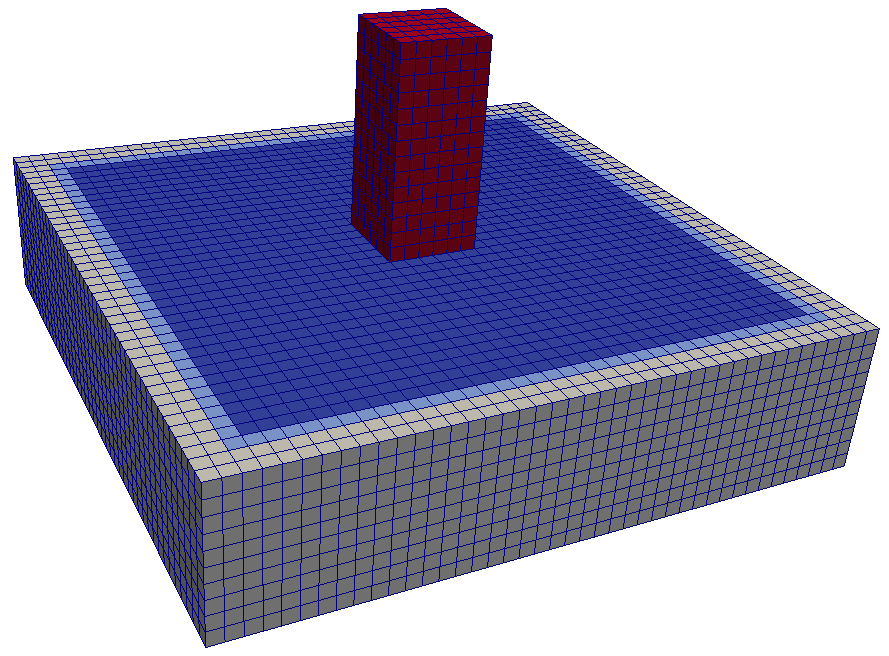
\includegraphics[width = 8cm]{./Figure-files/Day2/Deconvolution_1D_Motions/Earthquake_Soil-Structure_Interaction_3D_Model_with_DRM/overview.png}
  \caption{Simulation Model}
  \label{fig_decon_1D_motion_3D_model2}
\end{figure}


The illustration results of DRM 3D Solid Structure Model  under 1D motion is shown 
in Fig.~\ref{fig_decon_1D_motion_3D_model_solid_structure}. 

\begin{figure}[H]
  \centering
  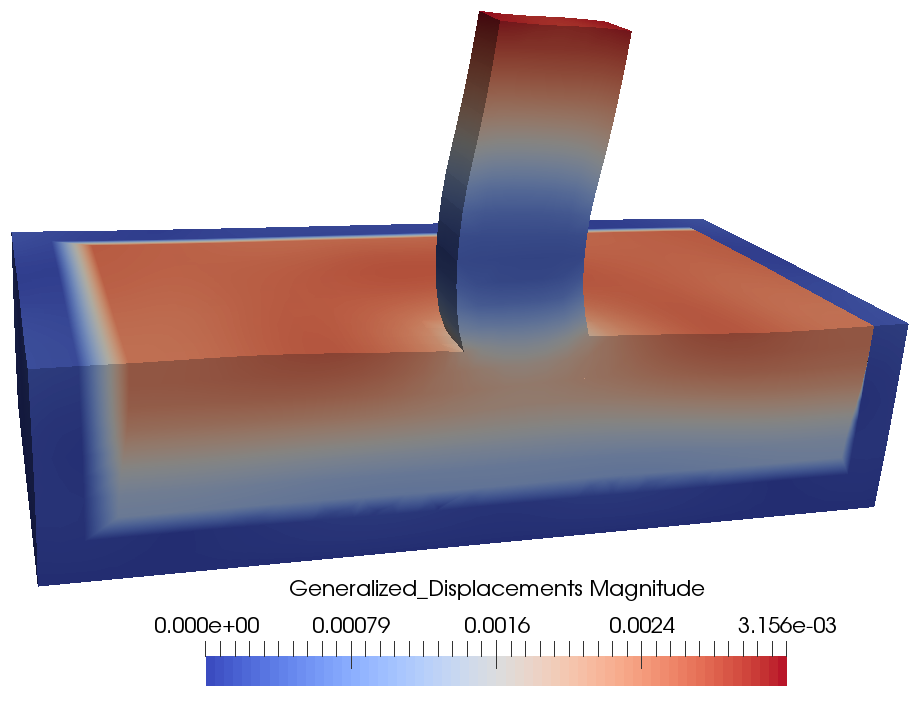
\includegraphics[width = 10cm]{./Figure-files/Day2/Deconvolution_1D_Motions/Earthquake_Soil-Structure_Interaction_3D_Model_with_DRM/DRM3D_results_1Dmotion.png}
  \caption{Simulation Model}
  \label{fig_decon_1D_motion_3D_model_solid_structure}
\end{figure}






% ******************************************************************
% ******************************************************************
% ******************************************************************
\clearpage
\newpage
\subsection{ESSI 3D building model, deconvolution 1D model, shell model with DRM}
\label{Earthquake_Soil-Structure_Interaction_3D_Model_with_DRM2}

The Real-ESSI input files for this example are available 
\href{http://sokocalo.engr.ucdavis.edu/~jeremic/lecture_notes_online_material/_Chapter_Short_Course_Examples/Day2/Deconvolution_1D_Motions/Shell_Structure_Soil_Interaction_3D_DRM}{HERE}. 
The compressed package of Real-ESSI input files for this example is available 
\href{http://sokocalo.engr.ucdavis.edu/~jeremic/lecture_notes_online_material/_Chapter_Short_Course_Examples/Day2/Deconvolution_1D_Motions/Shell_Structure_Soil_Interaction_3D_DRM/_all_files_packaged_for_Shell_Structure_Soil_Interaction_3D_DRM.tar.gz}{HERE}. 

The Modeling parameters are listed.
\begin{itemize}
  \item Elastic Soil Material Properties 
  \begin{itemize}
    \item Mass density, $\rho$, \enspace \enspace 2000 $kg/m^3$
    \item Shear Wave Velocity, $V_s$, \enspace \enspace 500 $m/s$
    \item Young's modulus, $E$, \enspace \enspace 1.1 GPa
    \item Poisson's ratio, $\nu$, \enspace \enspace 0.1
  \end{itemize}
  \item Elastic Structure Material Properties 
  \begin{itemize}
    \item Mass density, $\rho$, \enspace \enspace 2500 $kg/m^3$
    \item Young's modulus, $E$, \enspace \enspace 20 GPa
    \item Poisson's ratio, $\nu$, \enspace \enspace 0.1
  \end{itemize}
\end{itemize}

\begin{figure}[H]
  \centering
  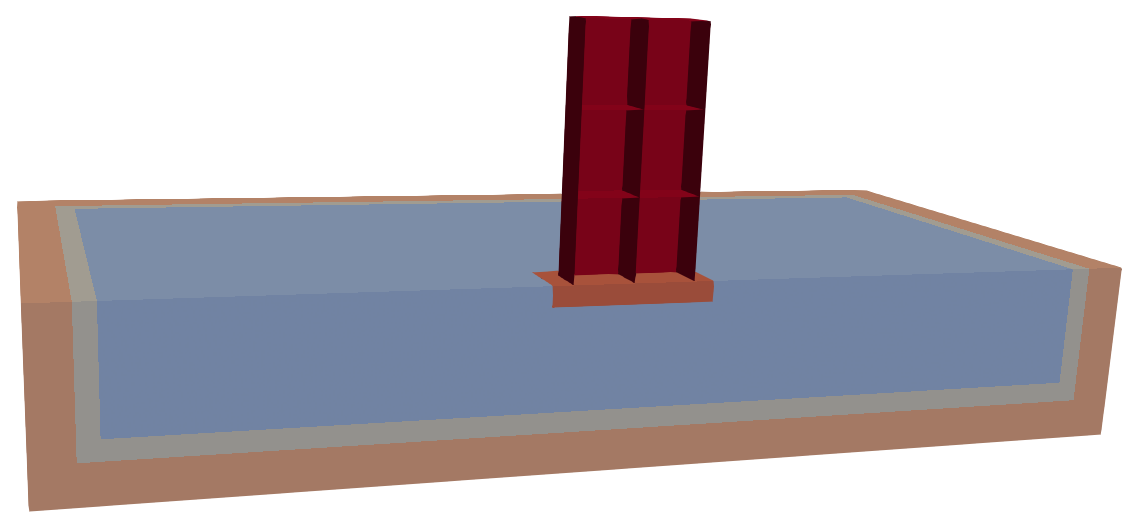
\includegraphics[width = 8cm]{./Figure-files/Day2/Deconvolution_1D_Motions/Shell_Structure_Soil_Interaction_3D_DRM/overview.png}
  \caption{Simulation Model}
  \label{fig_decon_1D_motion_3D_model_shell1}
\end{figure}


The illustration results of DRM 3D shell Structure Model under 1D motion is shown 
in Fig.~\ref{fig_decon_1D_motion_3D_model_solid_shell_structure}. 

\begin{figure}[H]
  \centering
  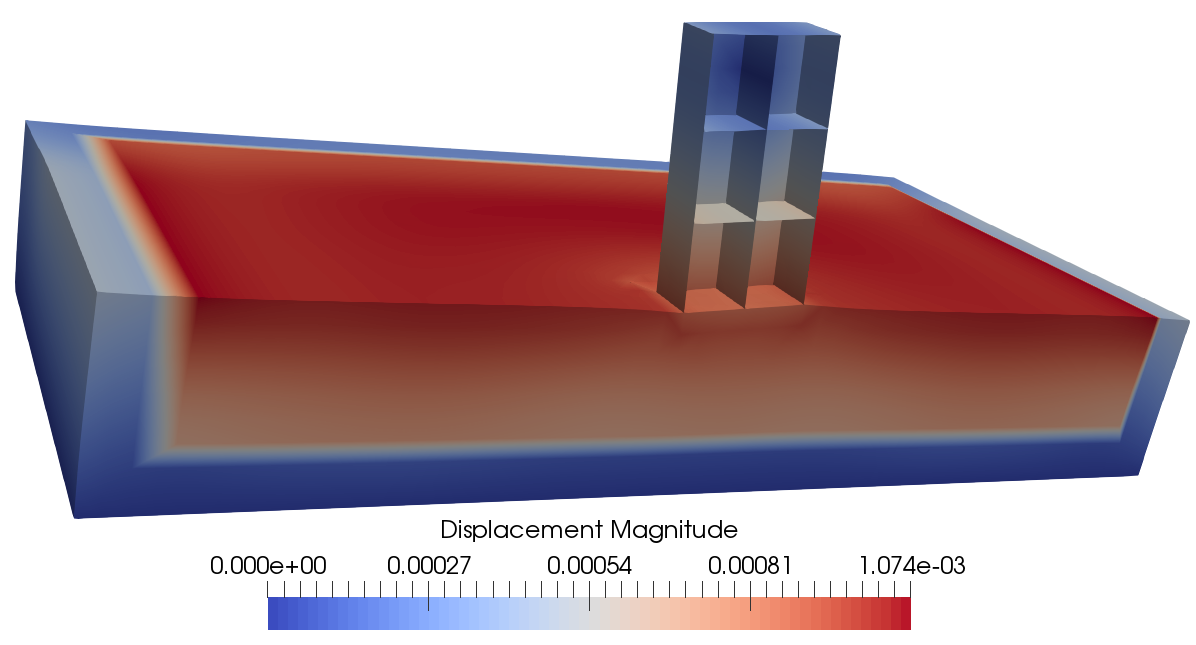
\includegraphics[width = 10cm]{./Figure-files/Day2/Deconvolution_1D_Motions/Shell_Structure_Soil_Interaction_3D_DRM/shell_DRM3D.png}
  \caption{Simulation Model}
  \label{fig_decon_1D_motion_3D_model_solid_shell_structure}
\end{figure}



























% ******************************************************************
% ******************************************************************
% ******************************************************************
\clearpage
\newpage
\section{Deconvolution 3$\times$1D Motions}
\label{Deconvolution_3by1D_Motions}
\subsection{Free field 1D model, deconvolution  3$\times$1D motion, model with DRM}
\label{Free_fields_1D_model_with_DRM2}

The Real-ESSI input files for this example are available 
\href{http://sokocalo.engr.ucdavis.edu/~jeremic/lecture_notes_online_material/_Chapter_Short_Course_Examples/Day2/Deconvolution_3by1D_Motions/Free_fields_1D_model_with_DRM}{HERE}. 
The compressed package of Real-ESSI input files for this example is available 
\href{http://sokocalo.engr.ucdavis.edu/~jeremic/lecture_notes_online_material/_Chapter_Short_Course_Examples/Day2/Deconvolution_3by1D_Motions/Free_fields_1D_model_with_DRM/_all_files_packaged_for_Free_fields_1D_model_with_DRM.tar.gz}{HERE}. 

The Modeling parameters are listed.
\begin{itemize}
  \item Elastic Material Properties 
  \begin{itemize}
    \item Mass density, $\rho$, \enspace \enspace 2000 $kg/m^3$
    \item Shear Wave Velocity, $V_s$, \enspace \enspace 500 $m/s$
    \item Young's modulus, $E$, \enspace \enspace 1.1 GPa
    \item Poisson's ratio, $\nu$, \enspace \enspace 0.1
  \end{itemize}
\end{itemize}

\begin{figure}[H]
  \centering
  \includegraphics[width = 0.8cm]{./Figure-files/Day2/Deconvolution_3by1D_Motions/Free_fields_1D_model_with_DRM/overview.png}
  \caption{Simulation Model}
  \label{fig_decon_1D_motion_1D_model2}
\end{figure}

The illustration results of the simulation is shown in Fig.~\ref{fig_decon_1D_motion_1D_model}.
As shown in the results, outside the DRM layer, there is no outgoing waves. 

\begin{figure}[H]
  \centering
  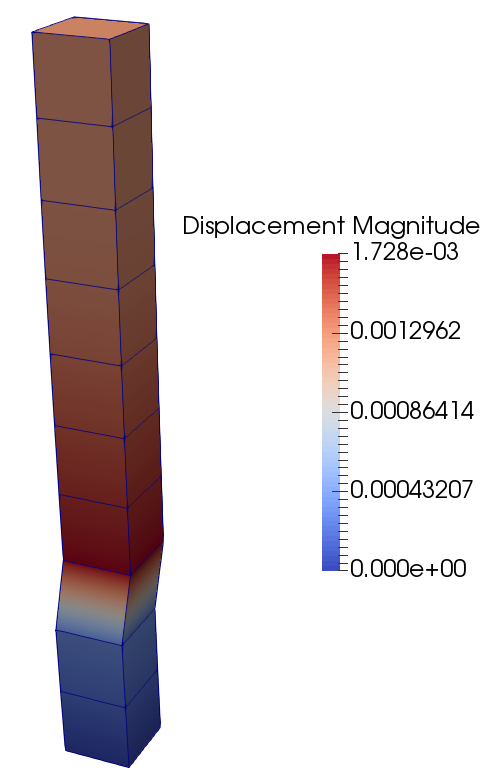
\includegraphics[width = 7cm]{./Figure-files/Day2/Deconvolution_3by1D_Motions/Free_fields_1D_model_with_DRM/DRM1D_Motion3D.png}
  \caption{Simulation Model}
  \label{fig_decon_3D_motion_1D_model_results}
\end{figure}


% ******************************************************************
% ******************************************************************
% ******************************************************************
\clearpage
\newpage
\subsection{Free field 3D model, deconvolution  3$\times$1D motion, model with DRM}
\label{Free_fields_3D_model_with_DRM2}

The Real-ESSI input files for this example are available 
\href{http://sokocalo.engr.ucdavis.edu/~jeremic/lecture_notes_online_material/_Chapter_Short_Course_Examples/Day2/Deconvolution_3by1D_Motions/Free_fields_3D_model_with_DRM}{HERE}. 
The compressed package of Real-ESSI input files for this example is available 
\href{http://sokocalo.engr.ucdavis.edu/~jeremic/lecture_notes_online_material/_Chapter_Short_Course_Examples/Day2/Deconvolution_3by1D_Motions/Free_fields_3D_model_with_DRM/_all_files_packaged_for_Free_fields_3D_model_with_DRM.tar.gz}{HERE}. 

The Modeling parameters are listed.
\begin{itemize}
  \item Elastic Soil Material Properties 
  \begin{itemize}
    \item Mass density, $\rho$, \enspace \enspace 2000 $kg/m^3$
    \item Shear Wave Velocity, $V_s$, \enspace \enspace 500 $m/s$
    \item Young's modulus, $E$, \enspace \enspace 1.1 GPa
    \item Poisson's ratio, $\nu$, \enspace \enspace 0.1
  \end{itemize}
\end{itemize}


\begin{figure}[H]
  \centering
  \includegraphics[width = 8cm]{./Figure-files/Day2/Deconvolution_3by1D_Motions/Free_fields_3D_model_with_DRM/overview.png}
  \caption{Simulation Model}
  \label{fig_decon_3by1D_motion_3D_model}
\end{figure}

The illustration results of the simulation is shown in Fig.~\ref{fig_decon_3D_motion_3D_model_results_free_field}.
As shown in the results, outside the DRM layer, there is no outgoing waves. 

\begin{figure}[H]
  \centering
  \includegraphics[width = 10cm]{./Figure-files/Day2/Deconvolution_3by1D_Motions/Free_fields_3D_model_with_DRM/motion3D_DRM3D_free_field.png}
  \caption{Simulation Model}
  \label{fig_decon_3D_motion_3D_model_results_free_field}
\end{figure}


% ******************************************************************
% ******************************************************************
% ******************************************************************
\clearpage
\newpage
\subsection{Free field 3D model, deconvolution  3$\times$1D motion, solid model with DRM}
\label{Earthquake_Soil-structure_interaction_3D_model_with_DRM3}

The Real-ESSI input files for this example are available 
\href{http://sokocalo.engr.ucdavis.edu/~jeremic/lecture_notes_online_material/_Chapter_Short_Course_Examples/Day2/Deconvolution_3by1D_Motions/Earthquake_Soil-Structure_Interaction_3D_Model_with_DRM}{HERE}. 
The compressed package of Real-ESSI input files for this example is available 
\href{http://sokocalo.engr.ucdavis.edu/~jeremic/lecture_notes_online_material/_Chapter_Short_Course_Examples/Day2/Deconvolution_3by1D_Motions/Earthquake_Soil-Structure_Interaction_3D_Model_with_DRM/_all_files_packaged_for_Earthquake_Soil-Structure_Interaction_3D_Model_with_DRM.tar.gz}{HERE}. 

The Modeling parameters are listed.
\begin{itemize}
  \item Elastic Soil Material Properties 
  \begin{itemize}
    \item Mass density, $\rho$, \enspace \enspace 2000 $kg/m^3$
    \item Shear Wave Velocity, $V_s$, \enspace \enspace 500 $m/s$
    \item Young's modulus, $E$, \enspace \enspace 1.1 GPa
    \item Poisson's ratio, $\nu$, \enspace \enspace 0.1
  \end{itemize}
  \item Elastic Structure Material Properties 
  \begin{itemize}
    \item Mass density, $\rho$, \enspace \enspace 2500 $kg/m^3$
    \item Young's modulus, $E$, \enspace \enspace 20 GPa
    \item Poisson's ratio, $\nu$, \enspace \enspace 0.1
  \end{itemize}
\end{itemize}

\begin{figure}[H]
  \centering
  \includegraphics[width = 8cm]{./Figure-files/Day2/Deconvolution_3by1D_Motions/Earthquake_Soil-Structure_Interaction_3D_Model_with_DRM/overview.png}
  \caption{Simulation Model}
  \label{fig_decon_1D_motion_3D_model3}
\end{figure}


The illustration results of the simulation is shown in Fig.~\ref{fig_decon_3D_motion_3D_model_results_structure}.
As shown in the results, outside the DRM layer, there is no outgoing waves. 

\begin{figure}[H]
  \centering
  \includegraphics[width = 10cm]{./Figure-files/Day2/Deconvolution_3by1D_Motions/Earthquake_Soil-Structure_Interaction_3D_Model_with_DRM/DRM3D_motion3D_structure.png}
  \caption{Simulation Model}
  \label{fig_decon_3D_motion_3D_model_results_structure}
\end{figure}





% ******************************************************************
% ******************************************************************
% ******************************************************************
\clearpage
\newpage
\subsection{ESSI 3D building model, deconvolution  3$\times$1D motion, shell model with DRM}
\label{Earthquake_Soil-Structure_Interaction_3D_Model_with_DRM4}

The Real-ESSI input files for this example are available 
\href{http://sokocalo.engr.ucdavis.edu/~jeremic/lecture_notes_online_material/_Chapter_Short_Course_Examples/Day2/Deconvolution_3by1D_Motions/Shell_Structure_Soil_Interaction_3D_DRM}{HERE}. 
The compressed package of Real-ESSI input files for this example is available 
\href{http://sokocalo.engr.ucdavis.edu/~jeremic/lecture_notes_online_material/_Chapter_Short_Course_Examples/Day2/Deconvolution_3by1D_Motions/Shell_Structure_Soil_Interaction_3D_DRM/_all_files_packaged_for_Shell_Structure_Soil_Interaction_3D_DRM.tar.gz}{HERE}. 

The Modeling parameters are listed.
\begin{itemize}
  \item Elastic Soil Material Properties 
  \begin{itemize}
    \item Mass density, $\rho$, \enspace \enspace 2000 $kg/m^3$
    \item Shear Wave Velocity, $V_s$, \enspace \enspace 500 $m/s$
    \item Young's modulus, $E$, \enspace \enspace 1.1 GPa
    \item Poisson's ratio, $\nu$, \enspace \enspace 0.1
  \end{itemize}
  \item Elastic Structure Material Properties 
  \begin{itemize}
    \item Mass density, $\rho$, \enspace \enspace 2500 $kg/m^3$
    \item Young's modulus, $E$, \enspace \enspace 20 GPa
    \item Poisson's ratio, $\nu$, \enspace \enspace 0.1
  \end{itemize}
\end{itemize}

\begin{figure}[H]
  \centering
  \includegraphics[width = 8cm]{./Figure-files/Day2/Deconvolution_3by1D_Motions/Shell_Structure_Soil_Interaction_3D_DRM/overview.png}
  \caption{Simulation Model}
  \label{fig_decon_3by1D_motion_3D_model_shell}
\end{figure}


The illustration results of DRM 3D shell Structure Model under 1D motion is shown 
in Fig.~\ref{fig_decon_3by1D_motion_3D_model_solid_shell_structure}. 

\begin{figure}[H]
  \centering
  \includegraphics[width = 10cm]{./Figure-files/Day2/Deconvolution_3by1D_Motions/Shell_Structure_Soil_Interaction_3D_DRM/DRM3D_motion3D_shell.png}
  \caption{Simulation Model}
  \label{fig_decon_3by1D_motion_3D_model_solid_shell_structure}
\end{figure}


















% ******************************************************************
% ******************************************************************
% ******************************************************************
\clearpage
\newpage
\section{Mesh Dependence of Wave Propagation Frequencies}
\label{Convolution_Motions}


The Real-ESSI input files for this example are available 
\href{http://sokocalo.engr.ucdavis.edu/~jeremic/lecture_notes_online_material/_Chapter_Short_Course_Examples/Day2/Convolution_Motions}{HERE}. 
The compressed package of Real-ESSI input files for this example is available 
\href{http://sokocalo.engr.ucdavis.edu/~jeremic/lecture_notes_online_material/_Chapter_Short_Course_Examples/Day2/Convolution_Motions/_all_files_packaged_for_Convolution_Motions.tar.gz}{HERE}. 


Show the mesh dependence of high frequency wave with Ormsby wavelet.

\begin{figure}[H]
  \centering
  \includegraphics[width = 0.5cm]{./Figure-files/Day2/Convolution_Motions/overview.png}
  \caption{Simulation Model}
  \label{fig_decon_1D_motion_3D_model4}
\end{figure}

The illustration results of mesh dependence is shown in Fig.~\ref{fig_day2_convolution_time_freq}.

\begin{figure}[H]
  \centering
  \includegraphics[width = 12cm]{./Figure-files/Day2/Convolution_Motions/top_acc_feq_all.pdf}
  \includegraphics[width = 12cm]{./Figure-files/Day2/Convolution_Motions/top_acc_time_all.pdf}
  \caption{Convolution Results and Mesh Dependence}
  \label{fig_day2_convolution_time_freq}
\end{figure}



































% ******************************************************************
% ******************************************************************
% ******************************************************************
\clearpage
\newpage
\section{Apply 3D Motions from SW4}
\label{Apply_3D_Motions_from_SW4}

\subsection{3D seismic motion by SW4}
\label{3D seismic motion by SW4}

A 3D seismic motion field has been developed by SW4. The characteristic parameters of the seismic motion are given below: 

\begin{itemize}
  \item Geological model:  length $3km$, width 3$km$, height $1.7km$, grid size $50m$, width of super grid damping layer $30m$.  
  \item Material model: Elastic material, First $1km$: $V_p= 4630.76m/s$, $V_s=2437.56m/s$, $\rho = 2600kg/m^3$.  $1km\sim1.7km$: $V_p=6000m/s$, $V_s=3464m/s$, $\rho = 2700kg/m^3$ 
  \item Source type: point moment source, moment seismic moment $M_{xy} = 5e^{15} N \cdot m$, moment magnitude 4.5. 
  \item Time function: Gaussian function, with dominant frequency $2.5Hz$ and maximum frequency $6.5Hz$. 
\end{itemize}  

The time series displacement and acceleration response at the center of the model is shown below in figure \ref{3D_motion_time_response}. 
%
And figure \ref{3D_motion_fft_response} gives corresponding FFT response. 

\begin{figure}[H]
  \centering
  \includegraphics[width = 8cm]{./Figure-files/Day2/Apply_3D_Motions_from_SW4/3D_seismic_motion_by_SW4/time_response.pdf}
  \caption{Time series response of 3D motion}
  \label{3D_motion_time_response}
\end{figure}

\begin{figure}[H]
  \centering
  \includegraphics[width = 8cm]{./Figure-files/Day2/Apply_3D_Motions_from_SW4/3D_seismic_motion_by_SW4/frequency_response.pdf}
  \caption{FFT response of 3D motion}
  \label{3D_motion_fft_response}
\end{figure}

During the simulation of SW4, the time series motions at many ESSI nodes (basically are some pre-defined record stations) of an ESSI box ($300m\times300m\times100m$) are recorded and written into \textbf{SAC} files. 
%
Then an transition program SW42ESSI has been developed to interpolate these motions to DRM nodes of localized ESSI model by specifying some geometric translational and rotational transformation, as shown in figure \ref{Transition from SW4 to Real ESSI}. 
%

To launch SW42ESSI, following parameters are needed: 

\begin{itemize}

  \item DRM input: specify the name of DRM input files. This DRM file just contains the geometric information of DRM layer in ESSI model (e.g. DRM node IDs, nodal coordinates, etc). 

  \item SW4 motion directory: specify the output directory of SW4, that contains SAC files. 

  \item origin coordinates of ESSI box (x, y, z): the SW4 coordinates of the origin of ESSI box, i.e. the coordinates of ESSI nodes, whose station ID is (0, 0, 0). 

  \item dimensions of ESSI Box (length, width, height): specify the dimension (length, width and height) of ESSI box. 

  \item spacing of ESSI nodes: specify the grid spacing of ESSI nodes (i.e. motion recording stations)

  \item interval of time steps for sampling: specify the sampling frequency, if 1 is used here, ESSI simulation time step is the same as the simulation time step of SW4.   

  \item reference point in ESSI model for translational transformation (x, y, z): specify the coordinate of reference point for translational transformation in ESSI model. 

  \item reference point in SW4 model for translational transformation (x, y, z): specify the coordinate of reference point for translational transformation in SW4 model. 

  \item conduct rotational transformation (yes/no): input yes and provide more rotational transformation parameters to enable rotational transformation. If input no, no more parameters are required.  

  \item reference point in SW4 model for rotational transformation (x, y, z): specify the coordinate of reference point for rotational transformation in SW4 model. 

  \item degrees of rotation along three axes (x, y, z): specify the degrees of rotation along three axes. The sign of rotation degrees follows right hand rule. 

\end{itemize}

\begin{figure}[H]
  \centering
  \includegraphics[width = \textwidth]{./Figure-files/Day2/Apply_3D_Motions_from_SW4/3D_seismic_motion_by_SW4/SW42DRM.pdf}
  \caption{Illustration of transition from SW4 to Real ESSI}
  \label{Transition from SW4 to Real ESSI}
\end{figure}


\subsection{Free field 3D model, 3D motion, model with DRM}
\label{Free_fields_3D_model_with_DRM3}


The Real-ESSI input files for this example are available 
\href{http://sokocalo.engr.ucdavis.edu/~jeremic/lecture_notes_online_material/_Chapter_Short_Course_Examples/Day2/Apply_3D_Motions_from_SW4/Free_fields_3D_model_with_DRM}{HERE}. 
The compressed package of Real-ESSI input files for this example is available 
\href{http://sokocalo.engr.ucdavis.edu/~jeremic/lecture_notes_online_material/_Chapter_Short_Course_Examples/Day2/Apply_3D_Motions_from_SW4/Free_fields_3D_model_with_DRM/_all_files_packaged_for_Free_fields_3D_model_with_DRM.tar.gz}{HERE}. 


\begin{figure}[H]
  \centering
  \includegraphics[width = 8cm]{./Figure-files/Day2/Apply_3D_Motions_from_SW4/Free_fields_3D_model_with_DRM/overview.png}
  \caption{Simulation Model}
  \label{fig_decon_1D_motion_3D_model5}
\end{figure}


The illustration results of free field DRM 3D Model under 3D motion is shown in figure \ref{3D_free_field_model_under_3D_motion}. 

\begin{figure}[H]
  \centering
  \includegraphics[width = 10cm]{./Figure-files/Day2/Apply_3D_Motions_from_SW4/Free_fields_3D_model_with_DRM/Free_field_model_3D_motion.pdf}
  \caption{Simulation of 3D free field model under 3D seismic motion}
  \label{3D_free_field_model_under_3D_motion}
\end{figure}



% ******************************************************************
% ******************************************************************
% ******************************************************************
\clearpage
\newpage
\subsection{ESSI 3D building model, 3D motion, solid model with DRM}
\label{Earthquake_Soil-Structure_Interaction_3D_Model_with_DRM5}

The Real-ESSI input files for this example are available 
\href{http://sokocalo.engr.ucdavis.edu/~jeremic/lecture_notes_online_material/_Chapter_Short_Course_Examples/Day2/Apply_3D_Motions_from_SW4/Earthquake_Soil-Structure_Interaction_3D_Model_with_DRM}{HERE}. 
The compressed package of Real-ESSI input files for this example is available 
\href{http://sokocalo.engr.ucdavis.edu/~jeremic/lecture_notes_online_material/_Chapter_Short_Course_Examples/Day2/Apply_3D_Motions_from_SW4/Earthquake_Soil-Structure_Interaction_3D_Model_with_DRM/_all_files_packaged_for_Earthquake_Soil-Structure_Interaction_3D_Model_with_DRM.tar.gz}{HERE}. 


\begin{figure}[H]
  \centering
  \includegraphics[width = 8cm]{./Figure-files/Day2/Apply_3D_Motions_from_SW4/Earthquake_Soil-Structure_Interaction_3D_Model_with_DRM/overview.png}
  \caption{Simulation Model}
  \label{fig_decon_1D_motion_3D_model6}
\end{figure}


The illustration results of DRM 3D Solid Structure Model  under 3D motion is shown in figure \ref{3D_solid_model_3D_seismic_motion}. 

\begin{figure}[H]
  \centering
  \includegraphics[width = 10cm]{./Figure-files/Day2/Apply_3D_Motions_from_SW4/Earthquake_Soil-Structure_Interaction_3D_Model_with_DRM/3D_solid_model_3D_motion.pdf}
  \caption{Simulation of 3D solid model under 3D seismic motions}
  \label{3D_solid_model_3D_seismic_motion}
\end{figure}




% ******************************************************************
% ******************************************************************
% ******************************************************************
\clearpage
\newpage
\subsection{ESSI 3D building model, 3D motion, shell model with DRM}
\label{Earthquake_Soil-Structure_Interaction_3D_Model_with_DRM6}

The Real-ESSI input files for this example are available 
\href{http://sokocalo.engr.ucdavis.edu/~jeremic/lecture_notes_online_material/_Chapter_Short_Course_Examples/Day2/Apply_3D_Motions_from_SW4/Shell_Structure_Soil_Interaction_3D_DRM}{HERE}. 
The compressed package of Real-ESSI input files for this example is available 
\href{http://sokocalo.engr.ucdavis.edu/~jeremic/lecture_notes_online_material/_Chapter_Short_Course_Examples/Day2/Apply_3D_Motions_from_SW4/Shell_Structure_Soil_Interaction_3D_DRM/_all_files_packaged_for_Shell_Structure_Soil_Interaction_3D_DRM.tar.gz}{HERE}. 


\begin{figure}[H]
  \centering
  \includegraphics[width = 8cm]{./Figure-files/Day2/Apply_3D_Motions_from_SW4/Shell_Structure_Soil_Interaction_3D_DRM/overview.png}
  \caption{Simulation Model}
  \label{fig_decon_1D_motion_3D_model_shell2}
\end{figure}


The illustration results of DRM 3D shell Structure Model under 3D seismic motion is shown in figure \ref{3D shell model under 3D seismic motion}. 

\begin{figure}[H]
  \centering
  \includegraphics[width = 10cm]{./Figure-files/Day2/Apply_3D_Motions_from_SW4/Shell_Structure_Soil_Interaction_3D_DRM/3D_shell_3D_motion.pdf}
  \caption{Simulation of 3D shell model under 3D motions}
  \label{3D shell model under 3D seismic motion}
\end{figure}


\chapter{Day 3 Nonlinearities}
\label{ch-day3}





% ******************************************************************
% ******************************************************************
% ******************************************************************
\clearpage
\newpage
\section{Single element Models: illustrate the elastic-plastic behavior}
\label{Single_element_Models_illustrate_the_elastic-plastic_behavior}
\subsection{von-Mises material model}


\paragraph{von-Mises perfectly plastic material model}
The Real-ESSI input files for von-Mises perfectly plastic example are available 
\href{http://sokocalo.engr.ucdavis.edu/~jeremic/lecture_notes_online_material/_Chapter_Short_Course_Examples/Day3/Single_element_Models_illustrate_the_elastic-plastic_behavior/vmpp}{HERE}. 
The compressed package of Real-ESSI input files for this example is available 
\href{http://sokocalo.engr.ucdavis.edu/~jeremic/lecture_notes_online_material/_Chapter_Short_Course_Examples/Day3/Single_element_Models_illustrate_the_elastic-plastic_behavior/vmpp/_all_files_packaged_for_vmpp.tar.gz}{HERE}. 

\paragraph{von-Mises Armstrong-Frederick material model}
The Real-ESSI input files for von-Mises Armstrong-Frederick example are available 
\href{http://sokocalo.engr.ucdavis.edu/~jeremic/lecture_notes_online_material/_Chapter_Short_Course_Examples/Day3/Single_element_Models_illustrate_the_elastic-plastic_behavior/vmaf}{HERE}. 
The compressed package of Real-ESSI input files for this example is available 
\href{http://sokocalo.engr.ucdavis.edu/~jeremic/lecture_notes_online_material/_Chapter_Short_Course_Examples/Day3/Single_element_Models_illustrate_the_elastic-plastic_behavior/vmaf/_all_files_packaged_for_vmaf.tar.gz}{HERE}. 


The Modeling parameters are listed.
\begin{itemize}
  \item Left: von-Mises linear hardening material model 
  \begin{itemize}
    \item Mass Density, $\rho$, \enspace \enspace 0.0 $kg/m^3$
    \item Young's modulus, $E$, \enspace \enspace 20 MPa
    \item Poisson's ratio, $\nu$, \enspace \enspace 0.0
    \item von Mises radius, $k$, \enspace \enspace 100 kPa
    \item kinematic hardening rate, $K_{kine} $, \enspace \enspace 2 MPa
    \item isotropic hardening rate, $K_{iso} $, \enspace \enspace 0 Pa
  \end{itemize}
  \item Right: Drucker-Prager nonlinear hardening material model 
  \begin{itemize}
    \item Mass Density, $\rho$, \enspace \enspace 0.0 $kg/m^3$
    \item Young's modulus, $E$, \enspace \enspace 20 MPa
    \item Poisson's ratio, $\nu$, \enspace \enspace 0.0
    \item Drucker-Prager, $k$, \enspace \enspace 0.179527
    \item nonlinear kinematic hardening, $H_a$, \enspace \enspace 20 MPa
    \item nonlinear kinematic hardening, $C_r$, \enspace \enspace 100
    \item isotropic hardening rate, $K_{iso} $, \enspace \enspace 0 Pa
    \item initial confining stress, $p_0$, \enspace \enspace 1 Pa
  \end{itemize}
\end{itemize}

\begin{figure}[H]
  \centering
  \includegraphics[width = 6cm]{./Figure-files/Day3/Single_element_Models_illustrate_the_elastic-plastic_behavior/overview.png}
  \caption{Simulation Model of Single Element}
  \label{fig_single_element_elastic_plastic1}
\end{figure}


The illustration results are shown in Fig.~\ref{fig_single_element_elastic_plastic_vmpp_vmaf}.

\begin{figure}[H]
  \centering
  \includegraphics[width = 7cm]{./Figure-files/Day3/Single_element_Models_illustrate_the_elastic-plastic_behavior/vmpp.pdf}
  \includegraphics[width = 7cm]{./Figure-files/Day3/Single_element_Models_illustrate_the_elastic-plastic_behavior/vmaf.pdf}
  \caption{Simulation Results of Single Element}
  \label{fig_single_element_elastic_plastic_vmpp_vmaf}
\end{figure}




% ******************************************************************
% ******************************************************************
% ******************************************************************
\clearpage
\newpage
\subsection{von-Mises G/Gmax material model}


The Real-ESSI input files for this example are available 
\href{http://sokocalo.engr.ucdavis.edu/~jeremic/lecture_notes_online_material/_Chapter_Short_Course_Examples/Day3/Single_element_Models_illustrate_the_elastic-plastic_behavior/vmGGmax}{HERE}. 
The compressed package of Real-ESSI input files for this example is available 
\href{http://sokocalo.engr.ucdavis.edu/~jeremic/lecture_notes_online_material/_Chapter_Short_Course_Examples/Day3/Single_element_Models_illustrate_the_elastic-plastic_behavior/vmGGmax/_all_files_packaged_for_vmGGmax.tar.gz}{HERE}. 

The Modeling parameters are listed.
\begin{itemize}
  \item von-Mises G/Gmax material model 
  \begin{itemize}
    \item Mass density, $\rho$, \enspace \enspace 2000 $kg/m^3$
    \item Young's modulus, $E$, \enspace \enspace 200 MPa
    \item Poisson's ratio, $\nu$, \enspace \enspace 0.1
    \item Total number of shear modulus \enspace \enspace  9
    \item G over Gmax, \enspace \enspace  1,0.995,0.966,0.873,0.787,0.467,0.320,0.109,0.063
    \item Shear strain gamma, \enspace \enspace  0,1E-6,1E-5,5E-5,1E-4, 0.0005, 0.001, 0.005, 0.01
  \end{itemize}
\end{itemize}


\begin{figure}[H]
  \centering
  \includegraphics[width = 3cm]{./Figure-files/Day3/Single_element_Models_illustrate_the_elastic-plastic_behavior/overview.png}
  \caption{Simulation Model of Single Element}
  \label{fig_single_element_elastic_plastic_vmGGmax}
\end{figure}



\begin{figure*}[!htbp]
    \centering
    \begin{subfigure}[b]{0.475\textwidth}
        \centering
        \includegraphics[width=\textwidth]{./Figure-files/Day3/Single_element_Models_illustrate_the_elastic-plastic_behavior/vmGGmax/1/backbone.pdf}
        \caption[]%
        {{\small Stress-Strain Curves}}    
    \end{subfigure}
    \hfill
    \begin{subfigure}[b]{0.475\textwidth}  
        \centering 
        \includegraphics[width=\textwidth]{./Figure-files/Day3/Single_element_Models_illustrate_the_elastic-plastic_behavior/vmGGmax/1/GGmax.pdf}
        \caption[]%
        {{\small G/Gmax Comparison}}    
    \end{subfigure}
    \vskip\baselineskip
    \begin{subfigure}[b]{0.475\textwidth}   
        \centering 
        \includegraphics[width=\textwidth]{./Figure-files/Day3/Single_element_Models_illustrate_the_elastic-plastic_behavior/vmGGmax/1/full-loop.pdf}
        \caption[]%
        {{\small One Cyclic Stress-Strain Curves}}    
    \end{subfigure}
    \quad
    \begin{subfigure}[b]{0.475\textwidth}   
        \centering 
        \includegraphics[width=\textwidth]{./Figure-files/Day3/Single_element_Models_illustrate_the_elastic-plastic_behavior/vmGGmax/1/damping.pdf}
        \caption[]%
        {{\small Damping Plot Curves}}    
    \end{subfigure}
    \caption[ Multi-Yield-Surface von-Mises]
    {\small Multi-Yield-Surface von-Mises} 
    \label{fig_Multi-Yield-Surface_von-Mises}
\end{figure*}




% ******************************************************************
% ******************************************************************
% ******************************************************************
\clearpage
\newpage
\subsection{Drucker-Prager perfectly plastic material model}

\paragraph{Drucker-Prager perfectly plastic material model}

The Real-ESSI input files for this Drucker-Prager perfectly plastic example are available 
\href{http://sokocalo.engr.ucdavis.edu/~jeremic/lecture_notes_online_material/_Chapter_Short_Course_Examples/Day3/Single_element_Models_illustrate_the_elastic-plastic_behavior/DPpp}{HERE}. 
The compressed package of Real-ESSI input files for this example is available 
\href{http://sokocalo.engr.ucdavis.edu/~jeremic/lecture_notes_online_material/_Chapter_Short_Course_Examples/Day3/Single_element_Models_illustrate_the_elastic-plastic_behavior/DPpp/_all_files_packaged_for_DPpp.tar.gz}{HERE}. 


\paragraph{Drucker-Prager Armstrong-Frederick Non-associate material model}

The Real-ESSI input files for this Drucker-Prager Armstrong-Frederick example are available 
\href{http://sokocalo.engr.ucdavis.edu/~jeremic/lecture_notes_online_material/_Chapter_Short_Course_Examples/Day3/Single_element_Models_illustrate_the_elastic-plastic_behavior/DPaf}{HERE}. 
The compressed package of Real-ESSI input files for this example is available 
\href{http://sokocalo.engr.ucdavis.edu/~jeremic/lecture_notes_online_material/_Chapter_Short_Course_Examples/Day3/Single_element_Models_illustrate_the_elastic-plastic_behavior/DPaf/_all_files_packaged_for_DPaf.tar.gz}{HERE}. 





\begin{figure}[H]
  \centering
  \includegraphics[width = 6cm]{./Figure-files/Day3/Single_element_Models_illustrate_the_elastic-plastic_behavior/overview.png}
  \caption{Simulation Model of Single Element}
  \label{fig_single_element_elastic_plastic2}
\end{figure}


The illustration results are shown in Fig.~\ref{fig_single_element_elastic_plastic_dppp_dpaf}.

\begin{figure}[H]
  \centering
  \includegraphics[width = 7cm]{./Figure-files/Day3/Single_element_Models_illustrate_the_elastic-plastic_behavior/dppp.pdf}
  \includegraphics[width = 7cm]{./Figure-files/Day3/Single_element_Models_illustrate_the_elastic-plastic_behavior/dpaf.pdf}
  \caption{Simulation Results of Single Element}
  \label{fig_single_element_elastic_plastic_dppp_dpaf}
\end{figure}




% ******************************************************************
% ******************************************************************
% ******************************************************************
\clearpage
\newpage
\subsection{Drucker-Prager G/Gmax Non-associate material model}



The Real-ESSI input files for this example are available 
\href{http://sokocalo.engr.ucdavis.edu/~jeremic/lecture_notes_online_material/_Chapter_Short_Course_Examples/Day3/Single_element_Models_illustrate_the_elastic-plastic_behavior/DPGGmax}{HERE}. 
The compressed package of Real-ESSI input files for this example is available 
\href{http://sokocalo.engr.ucdavis.edu/~jeremic/lecture_notes_online_material/_Chapter_Short_Course_Examples/Day3/Single_element_Models_illustrate_the_elastic-plastic_behavior/DPGGmax/_all_files_packaged_for_DPGGmax.tar.gz}{HERE}. 

The Modeling parameters are listed.
\begin{itemize}
  \item Drucker-Prager G/Gmax material model 
  \begin{itemize}
    \item Mass density, $\rho$, \enspace \enspace 2000 $kg/m^3$
    \item Young's modulus, $E$, \enspace \enspace 200 MPa
    \item Poisson's ratio, $\nu$, \enspace \enspace 0.1
    \item Initial confining stress, $p_0$, \enspace \enspace 100 kPa
    \item Reference pressure, $p_{refer} $, \enspace \enspace 100 kPa
    \item Pressure exponential, $ n  $, \enspace \enspace 0.5
    \item Cohesion, $ n  $, \enspace \enspace 1 kPa
    \item Total number of Shear Modulus \enspace \enspace 9
    \item G over Gmax, \enspace \enspace  1,0.995,0.966,0.873,0.787,0.467,0.320,0.109,0.063
    \item Shear strain gamma, \enspace \enspace  0,1E-6,1E-5,5E-5,1E-4, 0.0005, 0.001, 0.005, 0.01
  \end{itemize}
\end{itemize}

\begin{figure}[H]
  \centering
  \includegraphics[width = 6cm]{./Figure-files/Day3/Single_element_Models_illustrate_the_elastic-plastic_behavior/overview.png}
  \caption{Simulation Model of Single Element}
  \label{fig_single_element_elastic_plastic3}
\end{figure}


The illustration results are shown in Fig.~\ref{fig_single_element_elastic_plastic_dpGGmax}.

\begin{figure}[H]
  \centering
  \includegraphics[width = 7cm]{./Figure-files/Day3/Single_element_Models_illustrate_the_elastic-plastic_behavior/dpGGmax/1/GGmax.pdf}
  \includegraphics[width = 7cm]{./Figure-files/Day3/Single_element_Models_illustrate_the_elastic-plastic_behavior/dpGGmax/1/damping.pdf}
  \caption{Simulation Results of Single Element}
  \label{fig_single_element_elastic_plastic_dpGGmax}
\end{figure}



% ******************************************************************
% ******************************************************************
% ******************************************************************
\clearpage
\newpage
\section{Wave Propagation through elastoplastic Soil}
\label{Wave_Propagation_through_elastoplastic_Soil}


The Real-ESSI input files for this example are available 
\href{http://sokocalo.engr.ucdavis.edu/~jeremic/lecture_notes_online_material/_Chapter_Short_Course_Examples/Day3/Wave_Propagation_through_elastoplastic_Soil}{HERE}. 
The compressed package of Real-ESSI input files for this example is available 
\href{http://sokocalo.engr.ucdavis.edu/~jeremic/lecture_notes_online_material/_Chapter_Short_Course_Examples/Day3/Wave_Propagation_through_elastoplastic_Soil/_all_files_packaged_for_Wave_Propagation_through_elastoplastic_Soil.tar.gz}{HERE}. 

\begin{figure}[H]
  \centering
  \includegraphics[width = 0.6cm]{./Figure-files/Day3/Wave_Propagation_through_elastoplastic_Soil/overview.png}
  \caption{Wave Propagation through elastoplastic Soils}
  \label{fig_wave_propagation_elastoplastic}
\end{figure}


The displacement series at the surface are plotted in time and frequency domain.


\begin{figure}[H]
  \centering
  \includegraphics[width = 8cm]{./Figure-files/Day3/Wave_Propagation_through_elastoplastic_Soil/Displacement.pdf}
  \includegraphics[width = 8cm]{./Figure-files/Day3/Wave_Propagation_through_elastoplastic_Soil/Displacement_Spectrum.pdf}
  \caption{Simulation Results of Wave Propagation}
  \label{fig_elastic_plastic_wave_propagation}
\end{figure}


% \paragraph{Another Set of Solution with motion reduction}

% The displacement series with motion reduction are plotted in time and frequency domain.

% \begin{figure}[H]
%   \centering
%   \includegraphics[width = 8cm]{./Figure-files/Day3/Wave_Propagation_through_elastoplastic_Soil/2Displacement.pdf}
%   \includegraphics[width = 8cm]{./Figure-files/Day3/Wave_Propagation_through_elastoplastic_Soil/2Displacement_Spectrum.pdf}
%   \caption{Simulation Results of Wave Propagation (motion reduction)}
%   \label{fig_elastic_plastic_wave_propagation_Half}
% \end{figure}






% ******************************************************************
% ******************************************************************
% ******************************************************************
\clearpage
\newpage
\section{Contact Examples}
\label{Contact_Examples}
\subsection{ Axial behavior: Stress Based Contact Element}


\paragraph{Stress-Based Hard Contact Example}
The Real-ESSI input files for hard contact example are available 
\href{http://sokocalo.engr.ucdavis.edu/~jeremic/lecture_notes_online_material/_Chapter_Short_Course_Examples/Day3/Contact_Examples/axial/HardContact_Elastic_Perfectly_Plastic_Shear_Model}{HERE}. 
The compressed package of Real-ESSI input files for this example is available 
\href{http://sokocalo.engr.ucdavis.edu/~jeremic/lecture_notes_online_material/_Chapter_Short_Course_Examples/Day3/Contact_Examples/axial/HardContact_Elastic_Perfectly_Plastic_Shear_Model/_all_files_packaged_for_HardContact_Elastic_Perfectly_Plastic_Shear_Model.tar.gz}{HERE}. 

\paragraph{Stress-Based Soft Contact Example}
The Real-ESSI input files for soft contact example are available 
\href{http://sokocalo.engr.ucdavis.edu/~jeremic/lecture_notes_online_material/_Chapter_Short_Course_Examples/Day3/Contact_Examples/axial/SoftContact_Elastic_Perfectly_Plastic_Shear_Model}{HERE}. 
The compressed package of Real-ESSI input files for this example is available 
\href{http://sokocalo.engr.ucdavis.edu/~jeremic/lecture_notes_online_material/_Chapter_Short_Course_Examples/Day3/Contact_Examples/axial/SoftContact_Elastic_Perfectly_Plastic_Shear_Model/_all_files_packaged_for_SoftContact_Elastic_Perfectly_Plastic_Shear_Model.tar.gz}{HERE}. 


The axial behavior of hard contact and soft contact are illustrated in Fig.~\ref{fig_soft_hard_contact}.



\begin{figure}[H]
  \centering
  \includegraphics[width = 8cm]{./Figure-files/Day3/Contact_Examples/softcontact.pdf}
  \includegraphics[width = 8cm]{./Figure-files/Day3/Contact_Examples/hardcontact.pdf}
  \caption{Simulation Results of Soft Contact and Hard Contact}
  \label{fig_soft_hard_contact}
\end{figure}






% ******************************************************************
% ******************************************************************
% ******************************************************************
\clearpage
\newpage
\subsection{ Shear behavior: Stress Based Contact }


\paragraph{Stress-Based Elastic-perfectly plastic contact}
The Real-ESSI input files for the the elastic-perfectly plastic example are available 
\href{http://sokocalo.engr.ucdavis.edu/~jeremic/lecture_notes_online_material/_Chapter_Short_Course_Examples/Day3/Contact_Examples/shear/SoftContact_Elastic_Perfectly_Plastic_Shear_Model}{HERE}. 
The compressed package of Real-ESSI input files for this example is available 
\href{http://sokocalo.engr.ucdavis.edu/~jeremic/lecture_notes_online_material/_Chapter_Short_Course_Examples/Day3/Contact_Examples/shear/SoftContact_Elastic_Perfectly_Plastic_Shear_Model/_all_files_packaged_for_SoftContact_Elastic_Perfectly_Plastic_Shear_Model.tar.gz}{HERE}. 


\paragraph{Stress-Based Elastic-hardening contact}

The Real-ESSI input files for the elastic-hardening contact example are available 
\href{http://sokocalo.engr.ucdavis.edu/~jeremic/lecture_notes_online_material/_Chapter_Short_Course_Examples/Day3/Contact_Examples/shear/SoftContact_Nonlinear_Hardening_Shear_Model}{HERE}. 
The compressed package of Real-ESSI input files for this example is available 
\href{http://sokocalo.engr.ucdavis.edu/~jeremic/lecture_notes_online_material/_Chapter_Short_Course_Examples/Day3/Contact_Examples/shear/SoftContact_Nonlinear_Hardening_Shear_Model/_all_files_packaged_for_SoftContact_Nonlinear_Hardening_Shear_Model.tar.gz}{HERE}. 



\paragraph{Stress-Based Elastic-hardening-softening contact}

The Real-ESSI input files for the elastic-hardening-softening example are available 
\href{http://sokocalo.engr.ucdavis.edu/~jeremic/lecture_notes_online_material/_Chapter_Short_Course_Examples/Day3/Contact_Examples/shear/SoftContact_Nonlinear_Hardening_Softening_Shear_Model}{HERE}. 
The compressed package of Real-ESSI input files for this example is available 
\href{http://sokocalo.engr.ucdavis.edu/~jeremic/lecture_notes_online_material/_Chapter_Short_Course_Examples/Day3/Contact_Examples/shear/SoftContact_Nonlinear_Hardening_Softening_Shear_Model/_all_files_packaged_for_SoftContact_Nonlinear_Hardening_Softening_Shear_Model.tar.gz}{HERE}. 



The axial behavior of hard contact and soft contact are illustrated in Fig.~\ref{fig_soft_hard_contact_shear}.


\begin{figure}[H]
  \centering
  \includegraphics[width = 8cm]{./Figure-files/Day3/Contact_Examples/shear_perfectly_plastic.pdf}
  \includegraphics[width = 8cm]{./Figure-files/Day3/Contact_Examples/shear_hard.pdf}
  \includegraphics[width = 8cm]{./Figure-files/Day3/Contact_Examples/shear_hard_soft.pdf}
  \caption{Simulation Results of Shear Bahaviors in Stress Based Contact Elements}
  \label{fig_soft_hard_contact_shear}
\end{figure}






% ******************************************************************
% ******************************************************************
% ******************************************************************
\clearpage
\newpage
\subsection{ Force Based Contact Example: Base Isolator}

The Real-ESSI input files for this example are available 
\href{http://sokocalo.engr.ucdavis.edu/~jeremic/lecture_notes_online_material/_Chapter_Short_Course_Examples/Day3/Contact_Examples/force_based}{HERE}. 
The compressed package of Real-ESSI input files for this example is available 
\href{http://sokocalo.engr.ucdavis.edu/~jeremic/lecture_notes_online_material/_Chapter_Short_Course_Examples/Day3/Contact_Examples/force_based/_all_files_packaged_for_force_based.tar.gz}{HERE}. 


\begin{figure}[H]
  \centering
  \includegraphics[width = 8cm]{./Figure-files/Day3/Contact_Examples/Model_Description.png}
  \caption{Simulation Model}
  \label{fig_contact_examples_base_isolator}
\end{figure}

The illustration results are show in Fig.\ref{fig_contact_examples_base_isolator_results}.


\begin{figure}[H]
  \centering
  \includegraphics[width = 8cm]{./Figure-files/Day3/Contact_Examples/Uniform_Acceleration_0_85_sec.png}
  \caption{Simulation Results of Contact Examples}
  \label{fig_contact_examples_base_isolator_results}
\end{figure}






% ******************************************************************
% ******************************************************************
% ******************************************************************
\clearpage
\newpage
\section{ Frame Pushover}
\label{Frame_Pushover}


The Real-ESSI input files for this example are available 
\href{http://sokocalo.engr.ucdavis.edu/~jeremic/lecture_notes_online_material/_Chapter_Short_Course_Examples/Day3/Frame_Pushover}{HERE}. 
The compressed package of Real-ESSI input files for this example is available 
\href{http://sokocalo.engr.ucdavis.edu/~jeremic/lecture_notes_online_material/_Chapter_Short_Course_Examples/Day3/Frame_Pushover/_all_files_packaged_for_Frame_Pushover.tar.gz}{HERE}. 


The Modeling parameters are listed.
\begin{itemize}
  \item Uniaxial concrete 
  \begin{itemize}
    \item Compressive strength,  \enspace \enspace 24 MPa
    \item Strain at compressive strength,  \enspace \enspace 0.001752
    \item Crushing strength,  \enspace \enspace 0.0 Pa
    \item Strain at compressive strength,  \enspace \enspace 0.003168
    \item lambda, \enspace \enspace 0.5
    \item Tensile strength, \enspace \enspace 0 Pa
    \item Tension softening stiffness, \enspace \enspace 0 Pa
  \end{itemize}
  \item Uniaxial steel
  \begin{itemize}
    \item Yield strength, \enspace \enspace 413.8 MPa
    \item Young's modulus, \enspace \enspace 200 GPa
    \item Strain hardening ratio, \enspace \enspace 0.01
    \item R0, \enspace \enspace 18.0
    \item cR1,  \enspace \enspace 0.925
    \item cR2,  \enspace \enspace 0.15
    \item a1, \enspace \enspace 0.0
    \item a2, \enspace \enspace 55.0
    \item a3, \enspace \enspace 0.0
    \item a4, \enspace \enspace 55.0
  \end{itemize}
\end{itemize}



\begin{figure}[H]
  \centering
  \includegraphics[width = 7cm]{./Figure-files/Day3/Frame_Pushover/overview.pdf}
  \includegraphics[width = 7cm]{./Figure-files/Day3/Frame_Pushover/rectangle_rebar2.pdf}
  \caption{Model of Pushover Simulation and the Cross Section of Fiber Beam (Concrete and Rebar) }
  \label{fig_frame_pushover}
\end{figure}

The illustrative result is shown in Fig.~\ref{fig_day3_fiberbeam_pushover_results}.

\begin{figure}[H]
  \centering
  \includegraphics[width = 8cm]{./Figure-files/Day3/Frame_Pushover/fiberBeamDeform.png}
  \caption{Illustration results of Fiber Pushover}
  \label{fig_day3_fiberbeam_pushover_results}
\end{figure}

\begin{figure}[H]
  \centering
  \includegraphics[width = 8cm]{./Figure-files/Day3/Frame_Pushover/boundary_condition_frame.png}
  \caption{Boundary Condition $u_x$ of Fiber Pushover}
  \label{fig_day1_fiberbeam_pushover_results_bc}
\end{figure}





% ******************************************************************
% ******************************************************************
% ******************************************************************
\clearpage
\newpage
\section{ Wall Pushover}
\label{Wall_Pushover}



The Real-ESSI input files for this example are available 
\href{http://sokocalo.engr.ucdavis.edu/~jeremic/lecture_notes_online_material/_Chapter_Short_Course_Examples/Day3/Wall_Pushover}{HERE}. 
The compressed package of Real-ESSI input files for this example is available 
\href{http://sokocalo.engr.ucdavis.edu/~jeremic/lecture_notes_online_material/_Chapter_Short_Course_Examples/Day3/Wall_Pushover/_all_files_packaged_for_Wall_Pushover.tar.gz}{HERE}. 


The Modeling parameters are listed.
\begin{itemize}
  \item Concrete  Wall
  \begin{itemize}
    \item Young's modulus, \enspace \enspace 36.9 GPa
    \item Poisson's ratio, \enspace \enspace 0.2
    \item Tensile yield strength, \enspace \enspace 5 MPa
    \item Compressive yield strength, \enspace \enspace 56 MPa
    \item Plastic deformation rate, \enspace \enspace 0.4
    \item Damage parameter Ap, \enspace \enspace 0.1
    \item Damage parameter An, \enspace \enspace 1.5
    \item Damage parameter Bn, \enspace \enspace 0.75
  \end{itemize}
  \item Uniaxial steel
  \begin{itemize}
    \item Yield strength, \enspace \enspace 457.5 MPa
    \item Young's modulus, \enspace \enspace 200 GPa
    \item Strain hardening ratio, \enspace \enspace 0.011042
    \item a1, \enspace \enspace 0.0
    \item a2, \enspace \enspace 55.0
    \item a3, \enspace \enspace 0.0
    \item a4, \enspace \enspace 55.0
  \end{itemize}
\end{itemize}


\begin{figure}[H]
  \centering
  \includegraphics[width = 7cm]{./Figure-files/Day3/Wall_Pushover/overview.pdf}
  \caption{Illustrative Model of Wall Element Pushover Simulation }
  \label{fig_frame_pushover_wall}
\end{figure}


% ******************************************************************
% ******************************************************************
% ******************************************************************
\clearpage
\newpage
\section{ Viscous nonlinear behavior }
\label{Viscous_nonlinear_behavior}
% from small to very large

The Real-ESSI input files for this example are available 
\href{http://sokocalo.engr.ucdavis.edu/~jeremic/lecture_notes_online_material/_Chapter_Short_Course_Examples/Day3/Viscous_nonlinear_behavior/Rayleigh}{HERE}. 
The compressed package of Real-ESSI input files for this example is available 
\href{http://sokocalo.engr.ucdavis.edu/~jeremic/lecture_notes_online_material/_Chapter_Short_Course_Examples/Day3/Viscous_nonlinear_behavior/Rayleigh/_all_files_packaged_for_Rayleigh.tar.gz}{HERE}. 


\begin{figure}[H]
  \centering
  \includegraphics[width = 0.5cm]{./Figure-files/Day3/Viscous_nonlinear_behavior/overview.png}
  \caption{Simulation Model}
  \label{fig_contact_examples1}
\end{figure}

The illustrative result is shown in Fig.~\ref{fig_day3_viscous_damping} and Fig.~\ref{fig_day3_viscous_damping_high}.

\begin{figure}[H]
  \centering
  \includegraphics[width = 8cm]{./Figure-files/Day3/Viscous_nonlinear_behavior/Rayleigh001Displacement.pdf}
  \includegraphics[width = 8cm]{./Figure-files/Day3/Viscous_nonlinear_behavior/Rayleigh001Displacement_Spectrum.pdf}
  \caption{Illustration results of Low Viscous Damping}
  \label{fig_day3_viscous_damping}
\end{figure}

\begin{figure}[H]
  \centering
  \includegraphics[width = 8cm]{./Figure-files/Day3/Viscous_nonlinear_behavior/Rayleigh002Displacement.pdf}
  \includegraphics[width = 8cm]{./Figure-files/Day3/Viscous_nonlinear_behavior/Rayleigh002Displacement_Spectrum.pdf}
  \caption{Illustration results of High Viscous Damping}
  \label{fig_day3_viscous_damping_high}
\end{figure}




% ******************************************************************
% ******************************************************************
% ******************************************************************
\clearpage
\newpage
\section{ Numerical Damping Example }
\label{Numerical_Damping_Example}

The Real-ESSI input files for this example are available 
\href{http://sokocalo.engr.ucdavis.edu/~jeremic/lecture_notes_online_material/_Chapter_Short_Course_Examples/Day3/Numerical_Damping_Example/newmark}{HERE}. 
The compressed package of Real-ESSI input files for this example is available 
\href{http://sokocalo.engr.ucdavis.edu/~jeremic/lecture_notes_online_material/_Chapter_Short_Course_Examples/Day3/Numerical_Damping_Example/newmark/_all_files_packaged_for_newmark.tar.gz}{HERE}. 


\begin{figure}[H]
  \centering
  \includegraphics[width = 0.5cm]{./Figure-files/Day3/Numerical_Damping_Example/overview.png}
  \caption{Simulation Model}
  \label{fig_contact_examples2}
\end{figure}


The illustrative result is shown in Fig.~\ref{fig_day3_viscous_damping} and Fig.~\ref{fig_day3_numerical_damping_high} .

\begin{figure}[H]
  \centering
  \includegraphics[width = 8cm]{./Figure-files/Day3/Numerical_Damping_Example/newmark06Displacement.pdf}
  \includegraphics[width = 8cm]{./Figure-files/Day3/Numerical_Damping_Example/newmark06Displacement_Spectrum.pdf}
  \caption{Illustration results of Low numerical Damping}
  \label{fig_day3_numerical_damping}
\end{figure}

\begin{figure}[H]
  \centering
  \includegraphics[width = 8cm]{./Figure-files/Day3/Numerical_Damping_Example/newmark10Displacement.pdf}
  \includegraphics[width = 8cm]{./Figure-files/Day3/Numerical_Damping_Example/newmark10Displacement_Spectrum.pdf}
  \caption{Illustration results of High numerical Damping}
  \label{fig_day3_numerical_damping_high}
\end{figure}









% ******************************************************************
% ******************************************************************
% ******************************************************************
\clearpage
\newpage
\section{ Realistic Nuclear Power Plant Example with Nonlinearities}
\label{Realistic_Nuclear_Power_Plant_Example_with_Nonlinearities}


The Real-ESSI input files for this example are available 
\href{http://sokocalo.engr.ucdavis.edu/~jeremic/lecture_notes_online_material/_Chapter_Short_Course_Examples/Day3/Realiastic_Nuclear_Power_Plant_Example_with_Nonlinearities}{HERE}. 
The compressed package of Real-ESSI input files for this example is available 
\href{http://sokocalo.engr.ucdavis.edu/~jeremic/lecture_notes_online_material/_Chapter_Short_Course_Examples/Day3/Realiastic_Nuclear_Power_Plant_Example_with_Nonlinearities/_all_files_packaged_for_Realiastic_Nuclear_Power_Plant_Example_with_Nonlinearities.tar.gz}{HERE}. 

The Modeling parameters are listed.
\begin{itemize}
  \item Soil 
  \begin{itemize}
    \item Unit weight, $\gamma$, \enspace \enspace 21.4 kPa
    \item Shear velocity, $Vs$, \enspace \enspace 500 m/s
    \item Young's modulus, $E$, \enspace \enspace 1.3 GPa
    \item Poisson's ratio, $\nu$, \enspace \enspace 0.25
    \item Shear strength, $S_u$, \enspace \enspace 650 kPa
    \item von Mises radius, $k$, \enspace \enspace 60 kPa
    \item kinematic hardening, $H_a$, \enspace \enspace 30 MPa
    \item kinematic hardening, $C_r$, \enspace \enspace 25
  \end{itemize}
  \item Structure
  \begin{itemize}
    \item Unit weight, $\gamma$, \enspace \enspace 24 kPa
    \item Young's modulus, $E$, \enspace \enspace 20 GPa
    \item Poisson's ratio, $\nu$, \enspace \enspace 0.21
  \end{itemize}
  \item Contact 
  \begin{itemize}
    \item Initial axial stiffness, $k_n^{init}$,  \enspace \enspace  1e9 N/m
    \item Stiffening rate, $S_r$,  \enspace \enspace  1000 /m 
    \item Maximum axial stiffness, $k_n^{max}$,  \enspace \enspace  1e12 N/m
    \item Shear stiffness, $k_t$,  \enspace \enspace  1e7 N/m
    \item Axial viscous damping, $C_n$,  \enspace \enspace  100 $N\cdot s /m$
    \item Shear viscous damping, $C_t$,  \enspace \enspace  100 $N\cdot s /m$
    \item Friction ratio, $\mu$,  \enspace \enspace  0.25
  \end{itemize}
\end{itemize}



\begin{figure}[H]
  \centering
  \includegraphics[width = 10cm]{./Figure-files/Day3/Realiastic_Nuclear_Power_Plant_Example_with_Nonlinearities/overview.png}
  \caption{Simulation Model}
  \label{fig_contact_examples3}
\end{figure}



SIMULATION TIME: With 32 cores on AWS EC2 c4.8xlarge instance, the running time for this example is 30 hours.
\chapter{Nonlinear Analysis Steps}
\label{ch-nonlinear-analysis-steps}





% ******************************************************************
% ******************************************************************
% ******************************************************************
\clearpage
\newpage
\section{Free Field 1D}
\label{free_field_1D}
\paragraph{Elastic Material}
The Real-ESSI input files for elastic example are available 
\href{http://sokocalo.engr.ucdavis.edu/~jeremic/lecture_notes_online_material/_Chapter_Short_Course_Examples/nonlinear_analysis_steps/free_field_1D/elastic}{HERE}. 
The compressed package of input files is  
\href{http://sokocalo.engr.ucdavis.edu/~jeremic/lecture_notes_online_material/_Chapter_Short_Course_Examples/nonlinear_analysis_steps/free_field_1D/elastic/_all_files_packaged_for_elastic.tar.gz}{HERE}. 


The Modeling parameters are listed.
\begin{itemize}
  \item Elastic Material Properties 
  \begin{itemize}
    \item Mass Density, $\rho$, \enspace \enspace 2000 $kg/m^3$
    \item Shear wave velocity, $V_s$, \enspace \enspace 500 $m/s$
    \item Young's modulus, $E$, \enspace \enspace 1.1 GPa
    \item Poisson's ratio, $\nu$, \enspace \enspace 0.1
  \end{itemize}
\end{itemize}





\paragraph{Elastoplastic Material}
The Real-ESSI input files for elastoplastic material example are available 
\href{http://sokocalo.engr.ucdavis.edu/~jeremic/lecture_notes_online_material/_Chapter_Short_Course_Examples/nonlinear_analysis_steps/free_field_1D/elastoplastic}{HERE}. 
The compressed package of input files is  
\href{http://sokocalo.engr.ucdavis.edu/~jeremic/lecture_notes_online_material/_Chapter_Short_Course_Examples/nonlinear_analysis_steps/free_field_1D/elastoplastic/_all_files_packaged_for_elastoplastic.tar.gz}{HERE}. 

The Modeling parameters are listed.
\begin{itemize}
  \item von-Mises nonlinear hardening material model 
  \begin{itemize}
    \item Mass density, $\rho$, \enspace \enspace 2000 $kg/m^3$
    \item Shear wave velocity, $V_s$, \enspace \enspace 500 $m/s$
    \item Young's modulus, $E$, \enspace \enspace 1.1 GPa
    \item Poisson's ratio, $\nu$, \enspace \enspace 0.1
    \item von Mises radius, $k$, \enspace \enspace 60 kPa
    \item Nonlinear kinematic hardening, $H_a$, \enspace \enspace  30 MPa
    \item Nonlinear kinematic hardening, $C_r$, \enspace \enspace  60
    \item Shear strength ($\approx \sqrt{2/3}\ {H_a/C_r} $), $S_u$, \enspace \enspace 408 kPa
    \item Isotropic hardening rate, $K_{iso}$, \enspace \enspace 0 Pa
  \end{itemize}
\end{itemize}





\begin{figure}[H]
  \centering
  \includegraphics[width = 0.5cm]{./Figure-files/nonlinear_analysis_steps/free_field_1D/overview.png}
  \caption{Simulation Model}
  \label{fig_decon_1D_motion_1D_model}
\end{figure}

The illustration results of the simulation is shown in Fig.~\ref{fig_decon_1D_motion_1D_model}.
As shown in the results, outside the DRM layer, there is no outgoing waves. 

\begin{figure}[H]
  \centering
  \includegraphics[width = 6cm]{./Figure-files/nonlinear_analysis_steps/free_field_1D/DRM1D_Motion3D.png}
  \caption{Simulation Model}
  \label{fig_decon_3D_motion_1D_model_results}
\end{figure}


The time series of simulation results is shown in Fig.~\ref{fig_decon_3D_motion_1D_model_results_top_bottom_time_series}.
\begin{figure}[H]
  \centering
  \includegraphics[width = 15cm]{./Figure-files/nonlinear_analysis_steps/free_field_1D/DRM1D_motion_node_5_x_acce_compare.pdf}
  \caption{Simulation Results: Acceleration Time Series}
  \label{fig_decon_3D_motion_1D_model_results_top_bottom_time_series}
\end{figure}

The response spectrum of motion is shown in Fig.~\ref{fig_spectrum_freq_period_time_series}.
\begin{figure}[H]
  \centering
  \includegraphics[width = 15cm]{./Figure-files/nonlinear_analysis_steps/free_field_1D/DRM1D_motion_node_5_x_spectrum_freq.pdf}
  \includegraphics[width = 15cm]{./Figure-files/nonlinear_analysis_steps/free_field_1D/DRM1D_motion_node_5_x_spectrum_period.pdf}
  \caption{Simulation Results: Response Spectrum at Soil Top}
  \label{fig_spectrum_freq_period_time_series}
\end{figure}

% ******************************************************************
% ******************************************************************
% ******************************************************************
\clearpage
\newpage
\section{Free Field 3D}
\label{free_field_3D}

\paragraph{Elastic Material}
% The Real-ESSI input files for this example are available 
% \href{http://sokocalo.engr.ucdavis.edu/~jeremic/lecture_notes_online_material/_Chapter_Short_Course_Examples/nonlinear_analysis_steps/free_field_3D/elastic}{HERE}. 
The compressed package of input files is  
\href{http://sokocalo.engr.ucdavis.edu/~jeremic/lecture_notes_online_material/_Chapter_Short_Course_Examples/nonlinear_analysis_steps/free_field_3D/elastic/_all_files_packaged_for_elastic.tar.gz}{HERE}. 


The Modeling parameters are listed.
\begin{itemize}
  \item Elastic Material Properties 
  \begin{itemize}
    \item Mass density, $\rho$, \enspace \enspace 2000 $kg/m^3$
    \item Shear wave velocity, $V_s$, \enspace \enspace 500 $m/s$
    \item Young's modulus, $E$, \enspace \enspace 1.1 GPa
    \item Poisson's ratio, $\nu$, \enspace \enspace 0.1
  \end{itemize}
\end{itemize}


SIMULATION TIME: With 8 cores on AWS EC2 c4.2xlarge instance, the running time for this example is 5 minutes.

\paragraph{von-Mises Armstrong-Frederick Material}
% The Real-ESSI input files for this example are available 
% \href{http://sokocalo.engr.ucdavis.edu/~jeremic/lecture_notes_online_material/_Chapter_Short_Course_Examples/nonlinear_analysis_steps/free_field_3D/elastoplastic}{HERE}. 
The compressed package of input files is  
\href{http://sokocalo.engr.ucdavis.edu/~jeremic/lecture_notes_online_material/_Chapter_Short_Course_Examples/nonlinear_analysis_steps/free_field_3D/elastoplastic/_all_files_packaged_for_elastoplastic.tar.gz}{HERE}. 

The Modeling parameters are listed.
\begin{itemize}
  \item von-Mises nonlinear hardening material model 
  \begin{itemize}
    \item Mass density, $\rho$, \enspace \enspace 2000 $kg/m^3$
    \item Shear wave velocity, $V_s$, \enspace \enspace 500 $m/s$
    \item Young's modulus, $E$, \enspace \enspace 1.1 GPa
    \item Poisson's ratio, $\nu$, \enspace \enspace 0.1
    \item von Mises radius, $k$, \enspace \enspace 60 kPa
    \item Nonlinear kinematic hardening, $H_a$, \enspace \enspace  30 MPa
    \item Nonlinear kinematic hardening, $C_r$, \enspace \enspace  60
    \item Shear strength ($\approx \sqrt{2/3}\ {H_a/C_r} $), $S_u$, \enspace \enspace 408 kPa
    \item Isotropic hardening rate, $K_{iso}$, \enspace \enspace 0 Pa
  \end{itemize}
\end{itemize}

SIMULATION TIME: With 8 cores on AWS EC2 c4.2xlarge instance, the running time for this example is 17 minutes.

\paragraph{von-Mises G/Gmax Material}
% The Real-ESSI input files for vonMisesGoverGmax material example are available 
% \href{http://sokocalo.engr.ucdavis.edu/~jeremic/lecture_notes_online_material/_Chapter_Short_Course_Examples/nonlinear_analysis_steps/free_field_3D/vonMisesGoverGmax}{HERE}. 
The compressed package of input files is  
\href{http://sokocalo.engr.ucdavis.edu/~jeremic/lecture_notes_online_material/_Chapter_Short_Course_Examples/nonlinear_analysis_steps/free_field_3D/vonMisesGoverGmax/_all_files_packaged_for_vonMisesGoverGmax.tar.gz}{HERE}. 

The Modeling parameters are listed.
\begin{itemize}
  \item von-Mises G/Gmax material model 
  \begin{itemize}
    \item Mass density, $\rho$, \enspace \enspace 2000 $kg/m^3$
    \item Shear wave velocity, $V_s$, \enspace \enspace 500 $m/s$
    \item Young's modulus, $E$, \enspace \enspace 1.1 GPa
    \item Poisson's ratio, $\nu$, \enspace \enspace 0.1
    \item Total number of shear modulus \enspace \enspace  9
    \item G over Gmax, \enspace \enspace  1,0.995,0.966,0.873,0.787,0.467,0.320,0.109,0.063
    \item Shear strain gamma, \enspace \enspace  0,1E-6,1E-5,5E-5,1E-4, 0.0005, 0.001, 0.005, 0.01
  \end{itemize}
\end{itemize}


SIMULATION TIME: With 8 cores on AWS EC2 c4.2xlarge instance, the running time for this example is 565 minutes.

\paragraph{Drucker-Prager G/Gmax Material}
% The Real-ESSI input files for this example are available 
% \href{http://sokocalo.engr.ucdavis.edu/~jeremic/lecture_notes_online_material/_Chapter_Short_Course_Examples/nonlinear_analysis_steps/free_field_3D/DruckerPragerGoverGmax}{HERE}. 
The compressed package of input files is  
\href{http://sokocalo.engr.ucdavis.edu/~jeremic/lecture_notes_online_material/_Chapter_Short_Course_Examples/nonlinear_analysis_steps/free_field_3D/DruckerPragerGoverGmax/_all_files_packaged_for_DruckerPragerGoverGmax.tar.gz}{HERE}. 

The Modeling parameters are listed.
\begin{itemize}
  \item Drucker-Prager G/Gmax material model 
  \begin{itemize}
    \item Mass density, $\rho$, \enspace \enspace 2000 $kg/m^3$
    \item Shear wave velocity, $V_s$, \enspace \enspace 500 $m/s$
    \item Young's modulus, $E$, \enspace \enspace 1.1 GPa
    \item Poisson's ratio, $\nu$, \enspace \enspace 0.1
    \item Initial confining stress, $p_0$, \enspace \enspace 100 kPa
    \item Reference pressure, $p_{refer} $, \enspace \enspace 100 kPa
    \item Pressure exponential, $ n  $, \enspace \enspace 0.5
    \item Cohesion, $ n  $, \enspace \enspace 1 kPa
    \item Total number of Shear Modulus \enspace \enspace 9
    \item G over Gmax, \enspace \enspace  1,0.995,0.966,0.873,0.787,0.467,0.320,0.109,0.063
    \item Shear strain gamma, \enspace \enspace  0,1E-6,1E-5,5E-5,1E-4, 0.0005, 0.001, 0.005, 0.01
  \end{itemize}
\end{itemize}


SIMULATION TIME: With 8 cores on AWS EC2 c4.2xlarge instance, the running time for this example is 565 minutes.




\begin{figure}[H]
  \centering
  \includegraphics[width = 8cm]{./Figure-files/nonlinear_analysis_steps/free_field_3D/overview.png}
  \caption{Simulation Model}
  \label{fig_nonlinear_motion_3D_model}
\end{figure}

The illustration results of the simulation is shown in Fig.~\ref{fig_decon_3D_motion_3D_model_results_free_field}.
As shown in the results, outside the DRM layer, there is no outgoing waves. 

\begin{figure}[H]
  \centering
  \includegraphics[width = 10cm]{./Figure-files/nonlinear_analysis_steps/free_field_3D/motion3D_DRM3D_free_field.png}
  \caption{Simulation Model}
  \label{fig_nonlinear_steps_D_motion_3D_model_results_free_field}
\end{figure}


The node tags of critical points for postprocessing are shown in Fig.\ref{fig_points_soil_foundation}.

\begin{figure}[H]
  \centering
  \includegraphics[width = 12cm]{./Figure-files/nonlinear_analysis_steps/free_field_3D/free_field_3D_node_location.pdf}
  \caption{Critical Points of Simulation Model}
  \label{fig_points_soil_foundation}
\end{figure}

SIMULATION TIME: With 8 cores on AWS EC2 c4.2xlarge instance, the running time for this example is 871 minutes.


The time series of simulation results is shown in Fig.~\ref{fig_decon_3D_motion_1D_model_results_top_bottom_time_series_fr3d}.
\begin{figure}[H]
  \centering
  \includegraphics[width = 15cm]{./Figure-files/nonlinear_analysis_steps/free_field_3D/DRM3D_motion_node_4454_x_acce_compare.pdf}
  \caption{Simulation Results: Acceleration Time Series }
  \label{fig_decon_3D_motion_1D_model_results_top_bottom_time_series_fr3d}
\end{figure}

The response spectrum of motion is shown in Fig.~\ref{fig_spectrum_freq_period_time_series_fr3d}.
\begin{figure}[H]
  \centering
  \includegraphics[width = 15cm]{./Figure-files/nonlinear_analysis_steps/free_field_3D/DRM3D_motion_node_4454_x_spectrum_freq.pdf}
  \includegraphics[width = 15cm]{./Figure-files/nonlinear_analysis_steps/free_field_3D/DRM3D_motion_node_4454_x_spectrum_period.pdf}
  \caption{Simulation Results: Response Spectrum at Soil Top}
  \label{fig_spectrum_freq_period_time_series_fr3d}
\end{figure}


% ******************************************************************
% ******************************************************************
% ******************************************************************
\clearpage
\newpage
\section{Soil-Foundation Interaction 3D}
\label{foundation_3D}


\paragraph{Elastic Material}
% The Real-ESSI input files for this example are available 
% \href{http://sokocalo.engr.ucdavis.edu/~jeremic/lecture_notes_online_material/_Chapter_Short_Course_Examples/nonlinear_analysis_steps/soil-foundation/elastic}{HERE}. 
The compressed package of input files is  
\href{http://sokocalo.engr.ucdavis.edu/~jeremic/lecture_notes_online_material/_Chapter_Short_Course_Examples/nonlinear_analysis_steps/soil-foundation/elastic/_all_files_packaged_for_elastic.tar.gz}{HERE}. 

The Modeling parameters are listed.
\begin{itemize}
  \item Elastic Material Properties 
  \begin{itemize}
    \item Mass density, $\rho$, \enspace \enspace 2000 $kg/m^3$
    \item Shear wave velocity, $V_s$, \enspace \enspace 500 $m/s$
    \item Young's modulus, $E$, \enspace \enspace 1.1 GPa
    \item Poisson's ratio, $\nu$, \enspace \enspace 0.1
  \end{itemize}
\end{itemize}

SIMULATION TIME: With 8 cores on AWS EC2 c4.2xlarge instance, the running time for this example is 13 minutes.

\paragraph{von-Mises Armstrong-Frederick Material}
% The Real-ESSI input files for this example are available 
% \href{http://sokocalo.engr.ucdavis.edu/~jeremic/lecture_notes_online_material/_Chapter_Short_Course_Examples/nonlinear_analysis_steps/soil-foundation/vonMisesArmstrongFrederick}{HERE}. 
The compressed package of input files is  
\href{http://sokocalo.engr.ucdavis.edu/~jeremic/lecture_notes_online_material/_Chapter_Short_Course_Examples/nonlinear_analysis_steps/soil-foundation/vonMisesArmstrongFrederick/_all_files_packaged_for_vonMisesArmstrongFrederick.tar.gz}{HERE}. 


The Modeling parameters are listed.
\begin{itemize}
  \item von-Mises nonlinear hardening material model 
  \begin{itemize}
    \item Mass density, $\rho$, \enspace \enspace 2000 $kg/m^3$
    \item Shear wave velocity, $V_s$, \enspace \enspace 500 $m/s$
    \item Young's modulus, $E$, \enspace \enspace 1.1 GPa
    \item Poisson's ratio, $\nu$, \enspace \enspace 0.1
    \item von Mises radius, $k$, \enspace \enspace 60 kPa
    \item Nonlinear kinematic hardening, $H_a$, \enspace \enspace  30 MPa
    \item Nonlinear kinematic hardening, $C_r$, \enspace \enspace  60
    \item Shear strength ($\approx \sqrt{2/3}\ {H_a/C_r} $), $S_u$, \enspace \enspace 408 kPa
    \item Isotropic hardening rate, $K_{iso}$, \enspace \enspace 0 Pa
  \end{itemize}
\end{itemize}


SIMULATION TIME: With 8 cores on AWS EC2 c4.2xlarge instance, the running time for this example is 36 minutes.


\paragraph{von-Mises G/Gmax Material}
% The Real-ESSI input files for this example are available 
% \href{http://sokocalo.engr.ucdavis.edu/~jeremic/lecture_notes_online_material/_Chapter_Short_Course_Examples/nonlinear_analysis_steps/soil-foundation/vonMisesGoverGmax}{HERE}. 
The compressed package of input files is  
\href{http://sokocalo.engr.ucdavis.edu/~jeremic/lecture_notes_online_material/_Chapter_Short_Course_Examples/nonlinear_analysis_steps/soil-foundation/vonMisesGoverGmax/_all_files_packaged_for_vonMisesGoverGmax.tar.gz}{HERE}. 

The Modeling parameters are listed.
\begin{itemize}
  \item von-Mises G/Gmax material model 
  \begin{itemize}
    \item Mass density, $\rho$, \enspace \enspace 2000 $kg/m^3$
    \item Shear wave velocity, $V_s$, \enspace \enspace 500 $m/s$
    \item Young's modulus, $E$, \enspace \enspace 1.1 GPa
    \item Poisson's ratio, $\nu$, \enspace \enspace 0.1
    \item Total number of shear modulus \enspace \enspace  9
    \item G over Gmax, \enspace \enspace  1,0.995,0.966,0.873,0.787,0.467,0.320,0.109,0.063
    \item Shear strain gamma, \enspace \enspace  0,1E-6,1E-5,5E-5,1E-4, 0.0005, 0.001, 0.005, 0.01
  \end{itemize}
\end{itemize}

SIMULATION TIME: With 8 cores on AWS EC2 c4.2xlarge instance, the running time for this example is 726 minutes.


\paragraph{Drucker-Prager G/Gmax Material}
% The Real-ESSI input files for this example are available 
% \href{http://sokocalo.engr.ucdavis.edu/~jeremic/lecture_notes_online_material/_Chapter_Short_Course_Examples/nonlinear_analysis_steps/soil-foundation/DruckerPragerGoverGmax}{HERE}. 
The compressed package of input files is  
\href{http://sokocalo.engr.ucdavis.edu/~jeremic/lecture_notes_online_material/_Chapter_Short_Course_Examples/nonlinear_analysis_steps/soil-foundation/DruckerPragerGoverGmax/_all_files_packaged_for_DruckerPragerGoverGmax.tar.gz}{HERE}. 


The Modeling parameters are listed.
\begin{itemize}
  \item Drucker-Prager G/Gmax material model 
  \begin{itemize}
    \item Mass density, $\rho$, \enspace \enspace 2000 $kg/m^3$
    \item Shear wave velocity, $V_s$, \enspace \enspace 500 $m/s$
    \item Young's modulus, $E$, \enspace \enspace 1.1 GPa
    \item Poisson's ratio, $\nu$, \enspace \enspace 0.1
    \item Initial confining stress, $p_0$, \enspace \enspace 100 kPa
    \item Reference pressure, $p_{refer} $, \enspace \enspace 100 kPa
    \item Pressure exponential, $ n  $, \enspace \enspace 0.5
    \item Cohesion, $ n  $, \enspace \enspace 1 kPa
    \item Total number of Shear Modulus \enspace \enspace 9
    \item G over Gmax, \enspace \enspace  1,0.995,0.966,0.873,0.787,0.467,0.320,0.109,0.063
    \item Shear strain gamma, \enspace \enspace  0,1E-6,1E-5,5E-5,1E-4, 0.0005, 0.001, 0.005, 0.01
  \end{itemize}
\end{itemize}

SIMULATION TIME: With 8 cores on AWS EC2 c4.2xlarge instance, the running time for this example is 1252 minutes.


\paragraph{Contact Elements}
% The Real-ESSI input files for contact element example are available 
% \href{http://sokocalo.engr.ucdavis.edu/~jeremic/lecture_notes_online_material/_Chapter_Short_Course_Examples/nonlinear_analysis_steps/soil-foundation/contact}{HERE}. 
The compressed package of input files is  
\href{http://sokocalo.engr.ucdavis.edu/~jeremic/lecture_notes_online_material/_Chapter_Short_Course_Examples/nonlinear_analysis_steps/soil-foundation/contact/_all_files_packaged_for_contact.tar.gz}{HERE}. 


The Modeling parameters are listed.
\begin{itemize}
  \item Elastic Material Properties 
  \begin{itemize}
    \item Mass density, $\rho$, \enspace \enspace 2000 $kg/m^3$
    \item Shear wave velocity, $V_s$, \enspace \enspace 500 $m/s$
    \item Young's modulus, $E$, \enspace \enspace 1.1 GPa
    \item Poisson's ratio, $\nu$, \enspace \enspace 0.1
  \end{itemize}
\end{itemize}

SIMULATION TIME: With 8 cores on AWS EC2 c4.2xlarge instance, the running time for this example is 24 minutes.

\paragraph{Both Elastoplastic Material and Contact Elements}
% The Real-ESSI input files for both elastoplastic material and contact element example are available 
% \href{http://sokocalo.engr.ucdavis.edu/~jeremic/lecture_notes_online_material/_Chapter_Short_Course_Examples/nonlinear_analysis_steps/soil-foundation/both_plastic_contact}{HERE}. 
The compressed package of input files is  
\href{http://sokocalo.engr.ucdavis.edu/~jeremic/lecture_notes_online_material/_Chapter_Short_Course_Examples/nonlinear_analysis_steps/soil-foundation/both_plastic_contact/_all_files_packaged_for_both_plastic_contact.tar.gz}{HERE}. 

SIMULATION TIME: With 8 cores on AWS EC2 c4.2xlarge instance, the running time for this example is 41 minutes.



\begin{figure}[H]
  \centering
  \includegraphics[width = 4cm]{./Figure-files/nonlinear_analysis_steps/soil-foundation/soil_foundation.png}
  \includegraphics[width = 12cm]{./Figure-files/nonlinear_analysis_steps/soil-foundation/soil_foundation.pdf}
  \caption{Simulation Model}
  \label{fig_foundation_only}
\end{figure}


The illustration results of the simulation is shown in Fig.~\ref{fig_decon_3D_motion_3D_model_results_structure}.
As shown in the results, outside the DRM layer, there is no outgoing waves. 

\begin{figure}[H]
  \centering
  \includegraphics[width = 10cm]{./Figure-files/nonlinear_analysis_steps/soil-foundation/foundation_results.png}
  \caption{Soil Foundation Interaction Results}
  \label{fig_soil_foundation_motion_3D_model_results_structure}
\end{figure}



The node tags of critical points for postprocessing are shown in Fig.\ref{fig_points_soil_foundation}.

\begin{figure}[H]
  \centering
  \includegraphics[width = 12cm]{./Figure-files/nonlinear_analysis_steps/soil-foundation/soil_foundation_node_location.pdf}
  \caption{Critical Points of Simulation Model}
  \label{fig_points_soil_foundation}
\end{figure}









% ******************************************************************
% ******************************************************************
% ******************************************************************
\clearpage
\newpage
\section{Soil-Structure Interaction 3D}
\label{ssi_3D}


\paragraph{Elastic Material}
% The Real-ESSI input files for elastic example are available 
% \href{http://sokocalo.engr.ucdavis.edu/~jeremic/lecture_notes_online_material/_Chapter_Short_Course_Examples/nonlinear_analysis_steps/soil-structure/elastic}{HERE}. 
The compressed package of input files is  
\href{http://sokocalo.engr.ucdavis.edu/~jeremic/lecture_notes_online_material/_Chapter_Short_Course_Examples/nonlinear_analysis_steps/soil-structure/elastic/_all_files_packaged_for_elastic.tar.gz}{HERE}. 

The Modeling parameters are listed.
\begin{itemize}
  \item Elastic Material Properties 
  \begin{itemize}
    \item Mass density, $\rho$, \enspace \enspace 2000 $kg/m^3$
    \item Shear wave velocity, $V_s$, \enspace \enspace 500 $m/s$
    \item Young's modulus, $E$, \enspace \enspace 1.1 GPa
    \item Poisson's ratio, $\nu$, \enspace \enspace 0.1
  \end{itemize}
\end{itemize}


SIMULATION TIME: With 8 cores on AWS EC2 c4.2xlarge instance, the running time for this example is 10 minutes.

\paragraph{von-Mises Armstrong-Frederick Material}
% The Real-ESSI input files for this example are available 
% \href{http://sokocalo.engr.ucdavis.edu/~jeremic/lecture_notes_online_material/_Chapter_Short_Course_Examples/nonlinear_analysis_steps/soil-structure/vonMisesArmstrongFrederick}{HERE}. 
The compressed package of input files is  
\href{http://sokocalo.engr.ucdavis.edu/~jeremic/lecture_notes_online_material/_Chapter_Short_Course_Examples/nonlinear_analysis_steps/soil-structure/vonMisesArmstrongFrederick/_all_files_packaged_for_vonMisesArmstrongFrederick.tar.gz}{HERE}. 


The Modeling parameters are listed.
\begin{itemize}
  \item von-Mises nonlinear hardening material model 
  \begin{itemize}
    \item Mass density, $\rho$, \enspace \enspace 2000 $kg/m^3$
    \item Shear wave velocity, $V_s$, \enspace \enspace 500 $m/s$
    \item Young's modulus, $E$, \enspace \enspace 1.1 GPa
    \item Poisson's ratio, $\nu$, \enspace \enspace 0.1
    \item von Mises radius, $k$, \enspace \enspace 60 kPa
    \item Nonlinear kinematic hardening, $H_a$, \enspace \enspace  30 MPa
    \item Nonlinear kinematic hardening, $C_r$, \enspace \enspace  60
    \item Shear strength ($\approx \sqrt{2/3}\ {H_a/C_r} $), $S_u$, \enspace \enspace 408 kPa
    \item Isotropic hardening rate, $K_{iso}$, \enspace \enspace 0 Pa
  \end{itemize}
\end{itemize}


SIMULATION TIME: With 8 cores on AWS EC2 c4.2xlarge instance, the running time for this example is 46 minutes.

\paragraph{von-Mises G/Gmax Material}
% The Real-ESSI input files for this example are available 
% \href{http://sokocalo.engr.ucdavis.edu/~jeremic/lecture_notes_online_material/_Chapter_Short_Course_Examples/nonlinear_analysis_steps/soil-structure/vonMisesGoverGmax}{HERE}. 
The compressed package of input files is  
\href{http://sokocalo.engr.ucdavis.edu/~jeremic/lecture_notes_online_material/_Chapter_Short_Course_Examples/nonlinear_analysis_steps/soil-structure/vonMisesGoverGmax/_all_files_packaged_for_vonMisesGoverGmax.tar.gz}{HERE}. 

The Modeling parameters are listed.
\begin{itemize}
  \item von-Mises G/Gmax material model 
  \begin{itemize}
    \item Mass density, $\rho$, \enspace \enspace 2000 $kg/m^3$
    \item Shear wave velocity, $V_s$, \enspace \enspace 500 $m/s$
    \item Young's modulus, $E$, \enspace \enspace 1.1 GPa
    \item Poisson's ratio, $\nu$, \enspace \enspace 0.1
    \item Total number of shear modulus \enspace \enspace  9
    \item G over Gmax, \enspace \enspace  1,0.995,0.966,0.873,0.787,0.467,0.320,0.109,0.063
    \item Shear strain gamma, \enspace \enspace  0,1E-6,1E-5,5E-5,1E-4, 0.0005, 0.001, 0.005, 0.01
  \end{itemize}
\end{itemize}

SIMULATION TIME: With 8 cores on AWS EC2 c4.2xlarge instance, the running time for this example is 755 minutes.

\paragraph{Drucker-Prager G/Gmax Material}
% The Real-ESSI input files for this example are available 
% \href{http://sokocalo.engr.ucdavis.edu/~jeremic/lecture_notes_online_material/_Chapter_Short_Course_Examples/nonlinear_analysis_steps/soil-structure/DruckerPragerGoverGmax}{HERE}. 
The compressed package of input files is  
\href{http://sokocalo.engr.ucdavis.edu/~jeremic/lecture_notes_online_material/_Chapter_Short_Course_Examples/nonlinear_analysis_steps/soil-structure/DruckerPragerGoverGmax/_all_files_packaged_for_DruckerPragerGoverGmax.tar.gz}{HERE}. 

SIMULATION TIME: With 8 cores on AWS EC2 c4.2xlarge instance, the running time for this example is 1178 minutes.

The Modeling parameters are listed.
\begin{itemize}
  \item Drucker-Prager G/Gmax material model 
  \begin{itemize}
    \item Mass density, $\rho$, \enspace \enspace 2000 $kg/m^3$
    \item Shear wave velocity, $V_s$, \enspace \enspace 500 $m/s$
    \item Young's modulus, $E$, \enspace \enspace 1.1 GPa
    \item Poisson's ratio, $\nu$, \enspace \enspace 0.1
    \item Initial confining stress, $p_0$, \enspace \enspace 100 kPa
    \item Reference pressure, $p_{refer} $, \enspace \enspace 100 kPa
    \item Pressure exponential, $ n  $, \enspace \enspace 0.5
    \item Cohesion, $ n  $, \enspace \enspace 1 kPa
    \item Total number of Shear Modulus \enspace \enspace 9
    \item G over Gmax, \enspace \enspace  1,0.995,0.966,0.873,0.787,0.467,0.320,0.109,0.063
    \item Shear strain gamma, \enspace \enspace  0,1E-6,1E-5,5E-5,1E-4, 0.0005, 0.001, 0.005, 0.01
  \end{itemize}
\end{itemize}

% SIMULATION TIME: With 8 cores, the running time for this example is 

\paragraph{Contact Elements}
% The Real-ESSI input files for this example are available 
% \href{http://sokocalo.engr.ucdavis.edu/~jeremic/lecture_notes_online_material/_Chapter_Short_Course_Examples/nonlinear_analysis_steps/soil-structure/contact}{HERE}. 
The compressed package of input files is  
\href{http://sokocalo.engr.ucdavis.edu/~jeremic/lecture_notes_online_material/_Chapter_Short_Course_Examples/nonlinear_analysis_steps/soil-structure/contact/_all_files_packaged_for_contact.tar.gz}{HERE}. 

SIMULATION TIME: With 8 cores on AWS EC2 c4.2xlarge instance, the running time for this example is 15 minutes.

\paragraph{Both Elastoplastic Material and Contact Elements}
% The Real-ESSI input files for both elastoplastic material and contact element example are available 
% \href{http://sokocalo.engr.ucdavis.edu/~jeremic/lecture_notes_online_material/_Chapter_Short_Course_Examples/nonlinear_analysis_steps/soil-structure/both_plastic_contact}{HERE}. 
The compressed package of input files is  
\href{http://sokocalo.engr.ucdavis.edu/~jeremic/lecture_notes_online_material/_Chapter_Short_Course_Examples/nonlinear_analysis_steps/soil-structure/both_plastic_contact/_all_files_packaged_for_both_plastic_contact.tar.gz}{HERE}. 





The thickness of the shell structure is 2 meters.

\begin{figure}[H]
  \centering
  \includegraphics[width = 7cm]{./Figure-files/nonlinear_analysis_steps/soil-structure/overview.png}
  \includegraphics[width = 14cm]{./Figure-files/nonlinear_analysis_steps/soil-structure/geometry.pdf}
  \caption{Simulation Model}
  \label{fig_decon_1D_motion_3D_model}
\end{figure}


The illustration results of the simulation is shown in Fig.~\ref{fig_decon_3D_motion_3D_model_results_structure}.
As shown in the results, outside the DRM layer, there is no outgoing waves. 

\begin{figure}[H]
  \centering
  \includegraphics[width = 12cm]{./Figure-files/nonlinear_analysis_steps/soil-structure/DRM3D_motion3D_structure.png}
  \caption{Simulation Model}
  \label{fig_decon_3D_motion_3D_model_results_structure}
\end{figure}

The node tags of critical points for postprocessing are shown in Fig.\ref{fig_points_3D_motion_3D_model_results_structure}.

\begin{figure}[H]
  \centering
  \includegraphics[width = 12cm]{./Figure-files/nonlinear_analysis_steps/soil-structure/soil-structure_node_location.pdf}
  \caption{Critical Points of Simulation Model}
  \label{fig_points_3D_motion_3D_model_results_structure}
\end{figure}

SIMULATION TIME: With 8 cores on AWS EC2 c4.2xlarge instance, the running time for this example is 47 minutes.

\paragraph{Simulation with 1D motion }
The time series of simulation results is shown in Fig.~\ref{fig_decon_3D_motion_1D_model_results_top_bottom_time_series_ssi3d_1D_motion}.
\begin{figure}[H]
  \centering
  \includegraphics[width = 15cm]{./Figure-files/nonlinear_analysis_steps/soil-structure-1D-ans/shell_structure_motion_node_38_x_acce_compare.pdf}
  \caption{Simulation Results: Acceleration Time Series with 1D motion}
  \label{fig_decon_3D_motion_1D_model_results_top_bottom_time_series_ssi3d_1D_motion}
\end{figure}

The response spectrum of motion is shown in Fig.~\ref{fig_spectrum_freq_period_time_series_ssi3d_1D_motion}.
\begin{figure}[H]
  \centering
  \includegraphics[width = 15cm]{./Figure-files/nonlinear_analysis_steps/soil-structure-1D-ans/shell_structure_motion_node_3195_x_spectrum_freq.pdf}
  \includegraphics[width = 15cm]{./Figure-files/nonlinear_analysis_steps/soil-structure-1D-ans/shell_structure_motion_node_3195_x_spectrum_period.pdf}
  \caption{Simulation Results: Response Spectrum of Structure Top with 1D motion}
  \label{fig_spectrum_freq_period_time_series_ssi3d_1D_motion}
\end{figure}


\paragraph{Simulation with 3 $\times$ 1D motion }
The time series of simulation results is shown in Fig.~\ref{fig_decon_3D_motion_1D_model_results_top_bottom_time_series_ssi3d_3D_motion}.
\begin{figure}[H]
  \centering
  \includegraphics[width = 15cm]{./Figure-files/nonlinear_analysis_steps/soil-structure-3D-ans/shell_structure_motion_node_38_x_acce_compare.pdf}
  \caption{Simulation Results: Acceleration Time Series with 3D motion}
  \label{fig_decon_3D_motion_1D_model_results_top_bottom_time_series_ssi3d_3D_motion}
\end{figure}

The response spectrum of motion is shown in Fig.~\ref{fig_spectrum_freq_period_time_series_ssi3d_3D_motion}.
\begin{figure}[H]
  \centering
  \includegraphics[width = 15cm]{./Figure-files/nonlinear_analysis_steps/soil-structure-3D-ans/shell_structure_motion_node_3195_x_spectrum_freq.pdf}
  \includegraphics[width = 15cm]{./Figure-files/nonlinear_analysis_steps/soil-structure-3D-ans/shell_structure_motion_node_3195_x_spectrum_period.pdf}
  \caption{Simulation Results: Response Spectrum of Structure Top with 3D motion}
  \label{fig_spectrum_freq_period_time_series_ssi3d_3D_motion}
\end{figure}


% ******************************************************************
% ******************************************************************
% ******************************************************************
\clearpage
\newpage
\section{Structure Analysis without Soil}
\label{structure_only_3D}

\subsection{Eigen Analysis}

The Real-ESSI input files for this example are available 
\href{http://sokocalo.engr.ucdavis.edu/~jeremic/lecture_notes_online_material/_Chapter_Short_Course_Examples/nonlinear_analysis_steps/structure/eigen}{HERE}. 
The compressed package of input files is  
\href{http://sokocalo.engr.ucdavis.edu/~jeremic/lecture_notes_online_material/_Chapter_Short_Course_Examples/nonlinear_analysis_steps/structure/eigen/_all_files_packaged_for_eigen.tar.gz}{HERE}. 



The thickness of the shell structure is 2 meters.
The simulation model is shown below.
\begin{figure}[H]
  \centering
  \includegraphics[width = 4cm]{./Figure-files/nonlinear_analysis_steps/structure/eigen/structure-only.png}
  \hspace{2cm}
  \includegraphics[width = 8cm]{./Figure-files/nonlinear_analysis_steps/structure/eigen/structure_geometry.pdf}
  \caption{Simulation Model}
  \label{fig_simulate_model}
\end{figure}


The eigen results:

\begin{figure}[H]
  \centering
  \includegraphics[width = 5cm]{./Figure-files/nonlinear_analysis_steps/structure/eigen/eigen1.png}
  \includegraphics[width = 5cm]{./Figure-files/nonlinear_analysis_steps/structure/eigen/eigen2.png}
  \includegraphics[width = 5cm]{./Figure-files/nonlinear_analysis_steps/structure/eigen/eigen3.png}
  \caption{Eigen Results (Eigen Mode 1 to 3 from left to right)}
  \label{fig_eigen_results_1}
\end{figure}


\begin{figure}[H]
  \centering
  \includegraphics[width = 5cm]{./Figure-files/nonlinear_analysis_steps/structure/eigen/eigen4.png}
  \includegraphics[width = 5cm]{./Figure-files/nonlinear_analysis_steps/structure/eigen/eigen5.png}
  \includegraphics[width = 5cm]{./Figure-files/nonlinear_analysis_steps/structure/eigen/eigen6.png}
  \caption{Eigen Results (Eigen Mode 4 to 6 from left to right)}
  \label{fig_eigen_results_2}
\end{figure}




% ******************************************************************
% ******************************************************************
% ******************************************************************
\clearpage
\newpage
\subsection{Imposed Motion}

The Real-ESSI input files for this example are available 
\href{http://sokocalo.engr.ucdavis.edu/~jeremic/lecture_notes_online_material/_Chapter_Short_Course_Examples/nonlinear_analysis_steps/structure/imposed_motion}{HERE}. 
The compressed package of input files is  
\href{http://sokocalo.engr.ucdavis.edu/~jeremic/lecture_notes_online_material/_Chapter_Short_Course_Examples/nonlinear_analysis_steps/structure/imposed_motion/_all_files_packaged_for_imposed_motion.tar.gz}{HERE}. 

The Modeling parameters are listed.
\begin{itemize}
  \item Elastic Material Properties 
  \begin{itemize}
    \item Mass density, $\rho$, \enspace \enspace 2000 $kg/m^3$
    \item Shear wave velocity, $V_s$, \enspace \enspace 500 $m/s$
    \item Young's modulus, $E$, \enspace \enspace 1.1 GPa
    \item Poisson's ratio, $\nu$, \enspace \enspace 0.1
  \end{itemize}
\end{itemize}


The thickness of the shell structure is 2 meters.
The simulation model is shown below.
\begin{figure}[H]
  \centering
  \includegraphics[width = 4cm]{./Figure-files/nonlinear_analysis_steps/structure/imposed_motion/structure-only.png}
  \hspace{2cm}
  \includegraphics[width = 8cm]{./Figure-files/nonlinear_analysis_steps/structure/eigen/structure_geometry.pdf}
  \caption{Simulation Model}
  \label{fig_simulate_model}
\end{figure}


The simulation results:

\begin{figure}[H]
  \centering
  \includegraphics[width = 5cm]{./Figure-files/nonlinear_analysis_steps/structure/imposed_motion/imposed_motion_results.png}
  \caption{Simulation Results}
  \label{fig_simulate}
\end{figure}


The time series of simulation results is shown in Fig.~\ref{fig_decon_3D_motion_1D_model_results_top_bottom_time_series_imposed_1D_motion}.
\begin{figure}[H]
  \centering
  \includegraphics[width = 15cm]{./Figure-files/nonlinear_analysis_steps/structure/imposed_motion/shell_structure_imposed_motion_node_38_x_acce_compare.pdf}
  \caption{Simulation Results: Acceleration Time Series with 1D imposed motion}
  \label{fig_decon_3D_motion_1D_model_results_top_bottom_time_series_imposed_1D_motion}
\end{figure}

The response spectrum of motion is shown in Fig.~\ref{fig_spectrum_freq_period_time_series_imposed_1D_motion}.
\begin{figure}[H]
  \centering
  \includegraphics[width = 15cm]{./Figure-files/nonlinear_analysis_steps/structure/imposed_motion/shell_structure_imposed_motion_node_38_x_spectrum_freq.pdf}
  \includegraphics[width = 15cm]{./Figure-files/nonlinear_analysis_steps/structure/imposed_motion/shell_structure_imposed_motion_node_38_x_spectrum_period.pdf}
  \caption{Simulation Results: Response Spectrum of Structure Top with 1D imposed motion}
  \label{fig_spectrum_freq_period_time_series_imposed_1D_motion}
\end{figure}


\chapter{Postprocessing Examples with Python}
\label{ch-post processing}

% \section{Python}

\section{Basic Operations on Output }

Real-ESSI output are stored in HDF5 file format. 
HDF5 file a binary file format, which has the internal directories of dataset.
To open a dataset in HDF5 output, one can open the HDF5 file with the python interface $h5py$.
Then, the dataset can be extracted by following the internal path in the HDF5 format.

\begin{lstlisting}[frame=single, language=Python]
import h5py
h5file = h5py.File(filename,'r')
time=h5file['/time'][()]
Element_Outputs = h5file['/Model/Elements/Element_Outputs'][:,:]
Gauss_Outputs = h5file['/Model/Elements/Gauss_Outputs'][:,:]
Index_to_Coordinates = h5file['/Model/Nodes/Index_to_Coordinates'][:,:]
Coordinates = h5file['/Model/Nodes/Coordinates'][:,:]
Index_to_Generalized_Displacements = \
h5file['/Model/Nodes/Index_to_Generalized_Displacements'][:,:]
Generalized_Displacements = \
h5file['/Model/Nodes/Generalized_Displacements'][:,:]
\end{lstlisting}

\section{Time Series Plotting}
Following the basic options on HDF5 outptu, suppose one already extracted the dataset
in the HDF5 output, then, the plot of the time series is illustrated below.
\begin{lstlisting}[frame=single, language=Python]
target_displacement = Generalized_Displacements[15]
plt.plot(time, target_displacement)
plt.xlabel("Time [s]")
plt.ylabel("Displacement [m]")
plt.grid()
plt.savefig("target_displacement_time_series.pdf")
plt.show()
\end{lstlisting}
Note that the output of Real-ESSI is always in the standard unit.

\section{Spectrum Analysis}
Furthermore, one can also extract the results and do spectrum analysis of 
the output.
\begin{lstlisting}[frame=single, language=Python]
import numpy as np
import matplotlib.pyplot as plt
import scipy.fftpack
import math
def FFT(x,dt,maxf,plot=True):
	# Number of samplepoints
	N = x.size;
	# Total Time 
	T = N*dt;
	# sample dpacing is dt
	# sampling frequency
	Fs = 1/dt;
	xfft  = scipy.fftpack.fft(x);
	xfreq = np.linspace(0.0, Fs/2, N/2);
	xfftHalf = 2.0/N * np.abs(xfft[:N//2]);
	xfftHalf[0] = xfftHalf[0]/2;
	if(plot):
		fig, ax = plt.subplots()
		ax.plot(xfreq, xfftHalf,'-k')
		if(maxf is not None):
			plt.xlim(0, maxf)
		plt.ylabel('Fourier transform |FFT(x)|')
		plt.xlabel('Frequency |Hz|')
		plt.show()
	return xfreq, xfftHalf
\end{lstlisting}

For advanced python scripts with Real-ESSI, please visit \url{https://github.com/SumeetSinha/Python-Scripts}.

% \clearpage
% \newpage
% \section{Matlab}








\clearpage
\newpage

\chapter{Summary}
\label{ch-summary}




% ********************************************************************
% ********************************************************************
% The Reference:

% \clearpage
% \newpage
% \nocite{*}
% \bibliographystyle{plainnat}
% % \bibliography{reference,refmech}
% \bibliography{reference}

%-------------------------------------------------------------------------------------------------------------%
%-------------------------------------------------------------------------------------------------------------%
\end{document}
